
% ===========================================================================
% Title:
% ---------------------------------------------------------------------------
% to create Type I fonts type "dvips -P cmz -t letter <filename>"
% ===========================================================================
\documentclass[11pt]{article}       %--- LATEX 2e base
\usepackage{latexsym}               %--- LATEX 2e base
\usepackage{comment}
\usepackage{url}
\usepackage{cleveref} %,colorlinks
\usepackage{mathtools}
\usepackage{multirow}
\usepackage{placeins}
\usepackage{float}
%\usepackage{amsthm}
\usepackage{hyperref}
\usepackage{fontspec}
\usepackage{listings}
\usepackage{xcolor}
\usepackage{lipsum}
\usepackage{graphicx}
\usepackage{algorithm}
\usepackage{blindtext}
\usepackage{subcaption}
\usepackage{enumitem}
\usepackage[numbers, sort]{natbib}
\usepackage{titlesec}

% By this gentlemen & scholar:
% http://tex.stackexchange.com/questions/60209/how-to-add-an-extra-level-of-sections-with-headings-below-subsubsection
\titleclass{\subsubsubsection}{straight}[\subsection]

\newcounter{subsubsubsection}[subsubsection]
\renewcommand\thesubsubsubsection{\thesubsubsection.\arabic{subsubsubsection}}
\renewcommand\theparagraph{\thesubsubsubsection.\arabic{paragraph}} % optional; useful if paragraphs are to be numbered

\titleformat{\subsubsubsection}
{\normalfont\normalsize\bfseries}{\thesubsubsubsection}{1em}{}
\titlespacing*{\subsubsubsection}
{0pt}{3.25ex plus 1ex minus .2ex}{1.5ex plus .2ex}

\makeatletter
\renewcommand\paragraph{\@startsection{paragraph}{5}{\z@}%
	{3.25ex \@plus1ex \@minus.2ex}%
	{-1em}%
	{\normalfont\normalsize\bfseries}}
\renewcommand\subparagraph{\@startsection{subparagraph}{6}{\parindent}%
	{3.25ex \@plus1ex \@minus .2ex}%
	{-1em}%
	{\normalfont\normalsize\bfseries}}
\def\toclevel@subsubsubsection{4}
\def\toclevel@paragraph{5}
\def\toclevel@paragraph{6}
\def\l@subsubsubsection{\@dottedtocline{4}{7em}{4em}}
\def\l@paragraph{\@dottedtocline{5}{10em}{5em}}
\def\l@subparagraph{\@dottedtocline{6}{14em}{6em}}
\makeatother

\setcounter{secnumdepth}{4}
\setcounter{tocdepth}{4}

% courtesy of this gentlemen and scholar:
% http://tex.stackexchange.com/questions/210284/how-to-write-pseudocode-similar-to-code-presented-in-beautiful-code-by-j-r-h
\definecolor{darkgray}{HTML}{404040}
\definecolor{rulegray}{HTML}{DADADA}
\definecolor{keywordblue}{HTML}{1F497C}

\lstdefinestyle{code}{
	basicstyle=\ttfamily,
	keywordstyle=\color{keywordblue},
	keywords={import,qualified,as,do,where},
	mathescape=true
}

\newcommand\clearlines[1]{%
	\if#10\else%
	\leavevmode\\%
	\expandafter\clearlines\expandafter{\the\numexpr#1-1}%
	\fi}

%---------------- Wide format -----------------------------------------------
\textwidth=6in \textheight=9in \oddsidemargin=0.25in
\evensidemargin=0.25in \topmargin=-0.5in
%--------------- Def., Theorem, Proof, etc. ---------------------------------
\newtheorem{definition}{Definition}
\newtheorem{theorem}{Theorem}
\newtheorem{lemma}{Lemma}
\newtheorem{claim}{Claim}
\newtheorem{corollary}{Corollary}
\newtheorem{property}{Property}
\newtheorem{observation}{Observation}
\newtheorem{fact}{Fact}
\newenvironment{proof}           {\noindent{\bf Proof.} }%
                                 {\null\hfill$\Box$\par\medskip}
\begin{comment}
%--------------- Algorithm --------------------------------------------------
\newtheorem{algX}{Algorithm}
\newenvironment{algorithm}       {\begin{algX}\begin{em}}%
                                 {\par\noindent --- End of Algorithm ---
                                 \end{em}\end{algX}}
\newcommand{\step}[2]            {\begin{list}{}
                                  {  \setlength{\topsep}{0cm}
                                     \setlength{\partopsep}{0cm}
                                     \setlength{\leftmargin}{0.8cm}
                                     \setlength{\labelwidth}{0.7cm}
                                     \setlength{\labelsep}{0.1cm}    }
                                  \item[#1]#2    \end{list}}
                                 % usage: \begin{algorithm} \label{xyz}
                                 %        ... \step{(1)}{...} ...
                                 %        \end{algorithm}
\end{comment}
%--------------- Figures ----------------------------------------------------


\newcommand{\includeFig}[3]      {\begin{figure}[htb] \begin{center}
                                 \includegraphics
                                 [width=4in,keepaspectratio] %comment this line to disable scaling
                                 {#2}\caption{\label{#1}#3} \end{center} \end{figure}}
                                 % usage: \includeFig{label}{file}{caption}

\def\sectionautorefname{Section}
\def\subsectionautorefname{Subsection}
\def\claimautorefname{Claim}
\def\algorithmautorefname{Algorithm}

% ===========================================================================
\begin{document}
% ===========================================================================

% ############################################################################
% Title
% ############################################################################

\title{Eikonal Solver for GPUs}


% ############################################################################
% Author(s) (no blank lines !)
\author{
% ############################################################################
Olivier Hamel\\
School of Computer Science\\
Carleton University\\
Ottawa, Canada K1S 5B6\\
{\em olivierhamel@cmail.carleton.ca}
% ############################################################################
} % end-authors
% ############################################################################

\maketitle

% ############################################################################
% Abstract
% ############################################################################
\begin{abstract}
We present a variant of the Fast Iterative Method\cite{jeong2008fast} similar to the Heap-Cell Method\cite{chacon2012fast}, which improves on FIM by prioritising block resolutions by their minimum possible arrival time. We demonstrate that this arrangement improves upon a naive Block FIM approach by avoiding non-productive block resolutions. We also provide experimental results running on commodity hardware for both ideal and pathological inputs.
\end{abstract}

\begin{comment}

Abstract

Intro
	introduce Eikonal equ & applications
	introduce FMM & parallelisability issues
	
	introduce project goal (HCM-on-GPU) & summary of results
	
	paper outline

Lit Review
	FMM & parallelisability
	FSM & drawbacks
	FIM & drawbacks
	HCM
	brief mention of other approaches which attempt to avoid wasting time processing things away from the causality front
	

General Approach
	HCM on a GPU (FMM scheduling of blocks, FIM solving of blocks)

Impl Details
	????

Results
	????

Conclusions
	????

Future Work
	Systolic Block Solver? Improved FIM impl?

\end{comment}



% ############################################################################
\section{Introduction} \label{sec:intro}
% ############################################################################

The Eikonal equation is a partial differential equation with numerous applications (e.g. pathfinding, seismic modelling, optimal control). While there exist a number of parallel algorithms for calculating numerical solutions for Eikonal equations, they typically assume infinite processors in their design.

We present a hybrid approach for GPU hardware which attempts to strike a balance between maximising the possible parallelism while minimising the total work. We achieve this by using a scheme similar to Block FIM\cite{jeong2008fast}, save that blocks are prioritised for execution based on their earliest possible arrival time. This ensures that we do not waste time processing candidates who are far ahead of our known wavefront. We show that the cost of maintaining this priority queue is worthwhile in practice both for large grid volumes ($2^{24} < $ grid points) and when attempting to solve certain Eikonal equations pathological to FIM.

An overview of the Eikonal equation is provided in \autoref{sec:eikonal}, and \autoref{sec:lit_review} lists previous work relevant to our design relevant.
\autoref{sec:design} and \autoref{sec:implementation} covers the design of our system and notable implementation details. \autoref{sec:results} details our testing hardware, the performance results of our approach on a number of test cases, and a comparison to other methods. \autoref{sec:conclusion} summarises our results, and lays out possible avenues for future work.

\begin{comment}
Introduce your project topic (start from parallel computing in
general and lead to your particular topic). Describe your project
goals. Describe what you have achieved in your project. Outline
the structure of your paper. (In Section~\ref{litrev}, we will
review the relevant literature. Section~\ref{projrep} will present
the results of our project. In Section~\ref{subsect1}, ...
Section~\ref{concl} concludes the paper.
\end{comment}







% ############################################################################
\section{Eikonal Equations} \label{sec:eikonal}
% ############################################################################

The Eikonal equation is a partial differential equation of the form:

\begin{equation}
|\nabla g(x)| = \frac{1}{f(x)}, \quad x \in R^n
\end{equation}
\begin{equation*}
|\nabla g(y)| = 0			  , \quad y \in \Omega \subseteq R^n
\end{equation*}

The equation describes the propagation of a wavefront from one or more sources. $g(x)$ denotes the time to the nearest-source to $x$, whilst $f(x)$ denotes the (positive) speed of the wavefront at $x$. $\Omega$ designates the set of sources.

We provide an approximation for $g(x)$ by defining a discrete Cartesian grid with $n$ dimensions. $h_{0 <= i < n}$ denotes the size of each grid point within this grid along the $i^{th}$ axis. A Godunov upwind difference scheme can be used to calculate a discretised solution of $g(x)$ by solving for $u(x)$ in $G(x) = 0$ where $G(x)$ defined as follows:\cite{zhao2005fast}
\begin{equation}\label{eq:godunov_first_order_discrete}
G(x) = \sum_{i=0}^{n}{(\frac{u(x) - u_{min_{i}}(x)}{h_i})^2} - (\frac{1}{f(x)})^2
\end{equation}
\begin{equation*}
u_{min_i}(x) = min(u(x - axis_i), u(x + axis_i))
\end{equation*}

Where $u(x)$ is the approximate solution calculated at grid point $x$. A grid point is said to be 'upwind' of another if it has a lower $u(x)$.

%In practice $h_i$ is held constant for all $i$ and factored along with the reciprocal into a 'cost' function 

\begin{comment}
Note that for our purposes we assume manhattan connectivity between grid points in the grid. It is possible to use other stencils.
<todo complete, require citation of relevant papers>
\end{comment}

\section{Literature Review} \label{sec:lit_review}

There are a number of algorithms and variants for finding numerical solutions to Eikonal PDE. The main three are the Fast Marching Method, the Fast Sweeping Method, and the Fast Iterative Method.

\subsection{Fast Marching Method (FMM)}\label{sec:FMM}\cite{tsitsiklis1995efficient}\cite{sethian1996fast}
The classic algorithm for solving Eikonal equations is the Fast Marching Method. It is a sequential label-setting algorithm extremely similar to Dijkstra's. The primary differences between them are that a node can enter a considered state without immediately progressing to the closed set, and the cost function considers flow from up to $n$ (in $R^n$) neighbour rather than simply the 'closest' one. Like Dijkstra its running time is bound by $O(|E| + |V| \cdot log(|V|))$ but due to the connectivity of the grid it is technically $O(|V| \cdot log(|V|))$ but effectively $O(w \cdot log(w)$ where $w$ is maximum wavefront size. It is worth noting that FMM has among the best upper bound on run-time when compared to other algorithms.

\subsection{Fast Sweeping Method (FSM)}\label{sec:FSM}\cite{zhao2005fast}
The Fast Sweeping Method is a label-correcting algorithm which (in its classic form) repeatedly sweeps forward and back along each axis in turn until the grid converges. For problems where the Eikonal is a weighted distance (i.e. $f(x) = c$ for all points) this requires no more than $2^n$ sweeps for $R^n$. In practice, the number of sweeps depends on how often characteristic curves' tangent change quadrant, which be prohibitively expensive. Even in near-ideal cases FSM is often outperformed by almost any other algorithm.\cite{jeong2008fast}\cite{gomez2015fast} Nevertheless, FSM offers one notable feature FMM and FIM lack: It requires no notion of an open-set to operate.

\subsection{Fast Iterative Method (FIM)}\label{sec:FIM}
The Fast Iterative Method is label-correcting algorithm designed for partial operation on GPUs. It maintains an unordered set of 'improvable' grid points and updates these in parallel on the GPU. Improving a grid point's $u(x)$ potentially improves their neighbours', and those who do improve are then (re-)inserted into the open set. This continues until the grid converges.

The use of an unordered open set avoids the sorting required to maintain the priority heap, while the label-correcting scheme permits parallel updates of entries in the open set. Overall FIM strikes a compromise between the brute force approach of FSM and the sequential precision of FMM.

In practice the Block FIM variant is used. Block FIM differs from FIM in that the grid is decomposed into non-overlapping $m^2$ blocks (for some $0 < m$) which are processed until every grid point within a block converged. Blocks invalidate their neighbours in the same manner as grid points. This arrangement exploits that most Eikonals' $f(x)$ are locally constant on a short scale (thus require few iterations to converge), improves memory coherence, and helps minimise the number of round-trips between the GPU and CPU. From here on 'FIM' implicitly refers to the block variant.

\subsection{(Parallel) Heap Cell Method (HCM, pHCM)}\label{sec:HCM}
The Heap Cell Method\cite{chacon2012fast} (and its parallelised variant, pHCM\cite{chacon2014parallel}) is a hybrid of FMM and FSM. FMM is used to schedule small blocks (termed \textit{cells}, typically $\le 2^8$) which are solved using FSM. Like Block FIM, this is to exploit that most speed fields are locally constant on a small scale, allowing effective use of FSM and reducing the problem size which must be tracked by FMM. This approach is extremely similar to our design, though it approaches the problem from the opposite direction: HCM uses FSM-on-small-blocks to reduce the cost of managing a priority heap, while we use a priority heap to reduce the number of block-solves.

\begin{comment}
classic algos: FMM, FSM, FIM

label setting (FMM) vs. label correcting (FSM, FIM)
\end{comment}



\begin{comment}
Give an overview of the relevant literature. Cite all relevant
papers, like \cite{DEL07}, \cite{PD07}, \cite{DER07}, \cite{LDR07},
\cite{DLX06}, \cite{CDE06}, and \cite{DFL06}. Outline for each paper
the relevant results in relation to your project. Make sure that you
don't just list all relevant papers in random order. Devise a scheme
to group papers by subject. The goal of this section is to present
to the reader the state-of-the-art in the field selected for your
project.
\end{comment}




% ############################################################################
\section{Design} \label{sec:design}
% ############################################################################

The main issue with FIM is that its design implicitly assumes infinite GPU parallelism. FIM's open set includes all blocks which might be improvable due to the previous iteration; this includes block which are 'far away' (causally speaking, see \autoref{fig:7_ring_4096_open_set}). Since FIM processes all blocks in its open set at every iteration this can lead to blocks being repeatedly solved without contributing to the final solution in any way. Rescheduling is useless in this case as it assumes that all tasks contribute to the final result, which is not true for FIM.

\begin{figure}
\centering
\begin{subfigure}[b]{.3\columnwidth}
	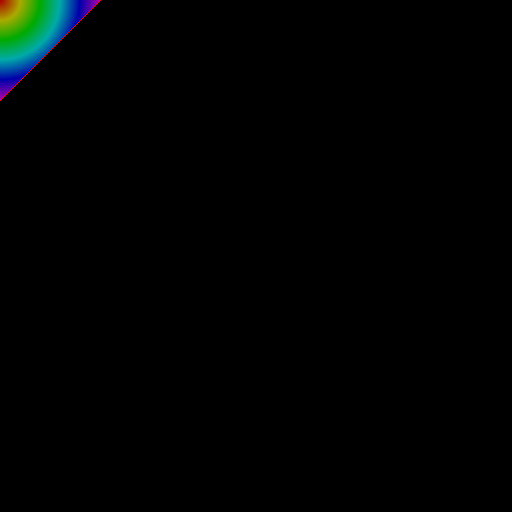
\includegraphics[width=\textwidth]{Figures/iter_100_fim}
	\caption{FIM Iter: 100}
\end{subfigure}
\begin{subfigure}[b]{.3\columnwidth}
	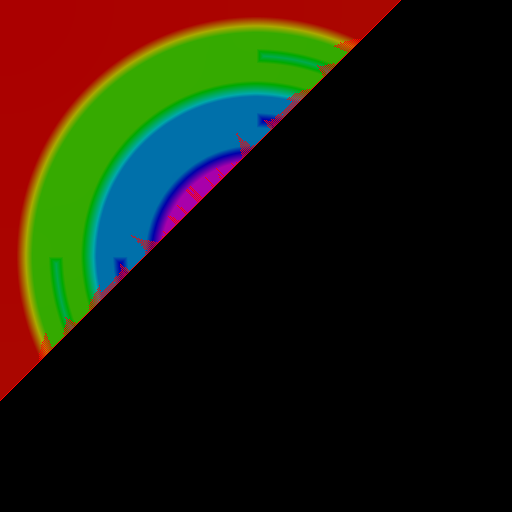
\includegraphics[width=\textwidth]{Figures/iter_400_fim}
	\caption{FIM Iter: 400}
\end{subfigure}
\begin{subfigure}[b]{.3\columnwidth}
	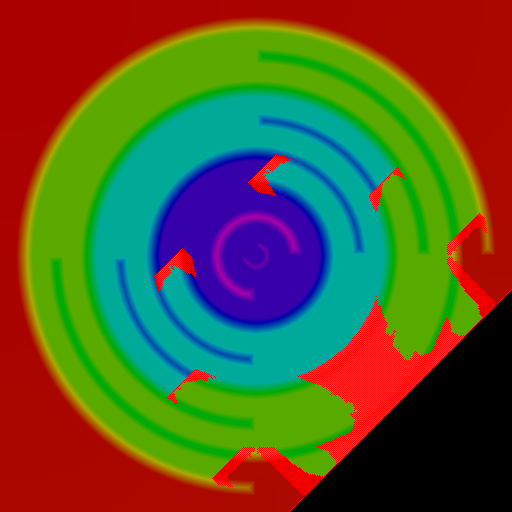
\includegraphics[width=\textwidth]{Figures/iter_800_fim}
	\caption{FIM Iter: 800}
\end{subfigure}

\begin{subfigure}[b]{.3\columnwidth}
	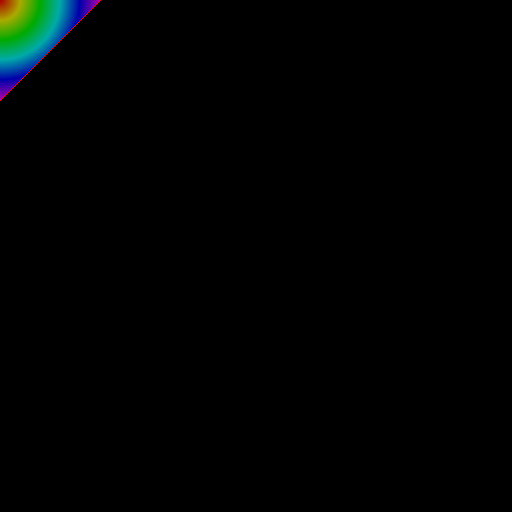
\includegraphics[width=\textwidth]{Figures/iter_100_ghcm}
	\caption{gHCM Iter: 100}
\end{subfigure}
\begin{subfigure}[b]{.3\columnwidth}
	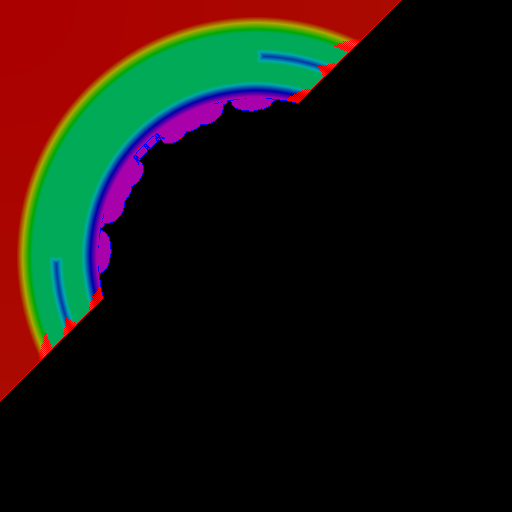
\includegraphics[width=\textwidth]{Figures/iter_400_ghcm}
	\caption{gHCM Iter: 400}
\end{subfigure}
\begin{subfigure}[b]{.3\columnwidth}
	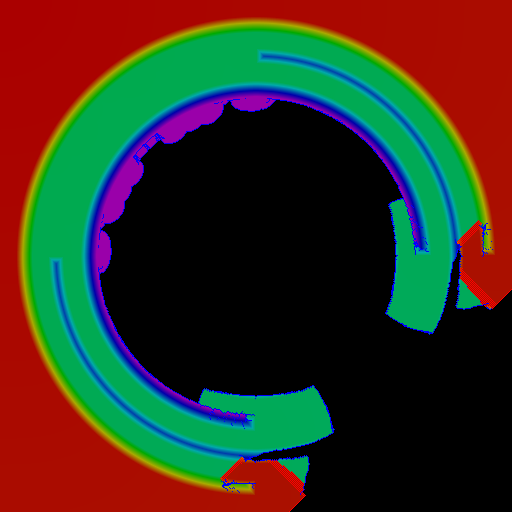
\includegraphics[width=\textwidth]{Figures/iter_800_ghcm}
	\caption{gHCM Iter: 800}
\end{subfigure}

\caption{Visualisation of the open-set and the current bundle at various iterations by FIM and gHCM (our approach). Bright blue pixels indicate blocks in the open-set. Bright red indicate blocks being processed this iteration. The minimum $u(x)$ is displayed hue'd in the background (muted) to visualise the label-correction as it progresses. FIM requires 2585 iterations and completes in 11728ms. gHCM requires 4325 iterations, but completes in only 3444ms.}
\label{fig:7_ring_4096_open_set}
\end{figure}

Our objective is therefore to avoid solving high minimum $u(x)$ blocks if there are lower $u(x)$ available in the open set. This implies we process a subset of the open-set at every iteration, the size of this subset being primarily dependent on the capabilities of the available hardware. We briefly confirm that this alteration does not impact the correctness of FIM.
\begin{claim}\label{claim:fim_can_solve_one_at_time}
(Non-Block) FIM remains correct so long as we process at least one entry of the open set per iteration.
\end{claim}
\begin{proof}
	
1) The $u(x)$ of any grid point is monotonically decreasing over multiple solves. (Proof in Jeong 2008\cite{jeong2008fast}.)

2) $0 \le u(x)$ for any grid point. ($0 \le f(x)$, $\forall x \in \Omega. u(x) = 0$)
\begin{comment}
This is iffy at best IMO. Replace all of this with an informal argument?
\end{comment}

Eventually no grid point will be valid for insertion into the open set. (Termination.)

If a grid point is no longer valid for insertion then it must have converged to its final $u(x)$ (within configurable $\epsilon$) given its neighbours. (By definition of FIM algorithm.)

Therefore by termination all grid point must have converged. Note that these properties do not depend on processing the entire open set at every iteration.
\end{proof}
\begin{claim}
Block FIM remains correct so long as we process at least entry of the open set.
\end{claim}
\begin{proof}
Same as for \autoref{claim:fim_can_solve_one_at_time}, as blocks are managed in the same manner as grid point.
\end{proof}


Our design (which we name 'gHCM' due to its similarity to HCM/pHCM) can be briefly described by the following pseudo-code:
\begin{algorithm}
\caption{Pseudo-code for gHCM.}
\label{alg:ghcm}
\begin{center}
	\footnotesize
	\begin{minipage}{.15\linewidth}
		\color{darkgray} \raggedleft \itshape
initialisation	\clearlines{7}
main loop		\clearlines{4}

	\end{minipage}
	\hfill{\color{rulegray}\vrule}\hfill
	\begin{minipage}{.83\linewidth}
		\begin{lstlisting}[style=code]
$\forall x \in grid.$ 	$u(x) := \infty$
$\forall x \in \Omega.$	 $\; u(x) := 0$
open-grid   $:= \big \{ \; x \; | \; x \in \bigcup\limits_{y \in \Omega}{\Gamma(y)} \; \big \} \;\; / \;\; \Omega $
open-blocks : PrioritySet Block
open-blocks $:= 	 \{ \; b \; | \; b \in blocks, \exists x \in b, x \in \text{open-grid} \; \} $

while $\neg$empty open-blocks:
  let (bundle, pending) = take $k$ open-blocks
  let dirtied-blocks    = parallel-fmap block-FIM-solve bundle
  open-blocks := merge pending dirtied-blocks
		\end{lstlisting}
	\end{minipage}

\end{center}
\end{algorithm}

\begin{comment}
Add defintion for block-FIM-solve?
\end{comment}

Indeed, it is effectively HCM but with a parallel block solving phase. pHCM differs from gHCM in that it features concurrent load-balancing priority queues on multiple processors which also solve the blocks, rather than a single priority queue on a single processor which dispatches to a GPU.

\subsection{Block Priority}

We define the priority of a block as follows:
\begin{equation}\label{eq:block_priority_func}
t(b) = min(\{ \; u(x) \; | \; x \in \{b\} \cup \Gamma(b) \; \})
\end{equation}

Where $\Gamma(b)$ is the neighbours of a block. We are interested in the earliest possible time the block $b$ might converge to; thus the $min$ of ourselves and our neighbours provides a good approximation that can be easily tracked \& updated per block while handling the cases where a block contains a source (always a good pick) or contains no sources and is considered for the first time (i.e. $min(\{ \; u(x) \; | \;  x \in b \} = \inf$).

\subsection{Blocks, Bundles, and Behaviour}
We replace FIM's open set with a min heap sorted on $t(b)$. We then select up to $k$ minimum entries, which we term 'bundles', and dispatch these to the GPU for solving.
\begin{comment}
Add pseudocode for algorithm?
\end{comment}
$k$, like the block size $m$, is a a user-configurable parameter. By varying the choice of $k$ and $m$ we can express the general behaviour of a number of other algorithms using our approach.
\begin{center}
\begin{table}[h]
\centering
\begin{tabular}{cr|c|c|c|}
\multirow{3}{*}{\rotatebox[origin=c]{90}{Max Block Size ($m$)}}		\\
	& \multicolumn{1}{r}{}	& \multicolumn{3}{c}{Max Bundle Size ($k$)}				\\
	&                  		& 1		& $[2, \infty)$						&  $\infty$	\\ \cline{2-5}
 	& 1						& FMM	& GMM-like\cite{kim2001levelset}	& FIM		\\ \cline{2-5} 
	& $[2, \infty)$			& HCM	& pHCM								& Block FIM	\\ \cline{2-5}
	& $\infty$				& FIM\footnotemark[0]	& -									& -			\\ \cline{2-5}
	\\
\end{tabular}
\caption{Various $m$ and $k$ limits causes our approach to behave similarly to the following algorithms.}
\label{tab:ghcm_behaviour_matrix}
\end{table}
\end{center}
\footnotetext[0]{This results in the entire problem being dispatch to the GPU as a single task. This might be feasible with OpenCL 2.0+ capable hardware, as these can enqueue kernels on the device without host intervention.}

\subsubsection{Bundle Size}\label{sec:bundle_size}
Picking an optimal $k$ depends on the chosen $m$, the size of the problem, the characteristic curves of the problem, and the characteristics of both the CPU and GPU. The lower $k$, the lower the number of average solves is required per block. Too low a $k$, however, and we loose our parallelism.\footnote{There are strong parallels between this conundrum and the Group Marching Method. However, we did not have time to consider its application to this sub-problem.} Whatever we choose we must also consider the cost of maintaining the priority heap.
\begin{equation} \label{eq:basic_ghcm_cost_model}
\begin{split}
z_k			&= E(\text{heap size of $gHCM_k$})					\\
s_x			&= E(\text{\# of solves for a block using $x$}) 	\\
c_x 		&= \text{cost of performing $x$}					\\
c_{fim}		&= c_{block} * s_{fim}								\\
c_{ghcm_k}	&= c_{block} * s_{ghcm_k} + c_{heap} * log_2(z_k)	\\
& \frac{c_{heap}}{c_{block}} * log_2(z_k) \le s_{fim} - s_{ghcm_k}
\end{split}
\end{equation}

For our method to outperform FIM the inequality in \autoref{eq:basic_ghcm_cost_model} must hold. $s$ and $z_k$ are both problem dependent; $z_k$ is also dependent on $k$ and the dimensionality of grid, and bound by the grid size divided by $m^n$ (for $R^n$).



\begin{comment}
start with FIM
	FIM chooses the following design:
		1) does not impose specific update sequence (limits parallelism)
		2) must be able to update multiple grid points in parallel (see 1)
		3) requires no sorting (no no on GPU)
		
	FIM sucks when the open-list fills up with blocks which are far away causally
		wastes time computing those when they'll eventually be recomputed w/ final info
		not a problem with infinite hardware, but we don't have infinite hardware
			rescheduling will not save you b/c these recomputes are useless (entirely invalidated by future updates)

objective:
	figure a way to avoid wasting time computing blocks ahead of the minimum current causality when there are causally nearby blocks avail
		-> basic idea is SSS-LLL (small labels soon, large labels last)

design:
	need to (untidy) order the blocks
		-> use a priority heap, peal off a bundle of K earliest possible blocks
			-> K = \# of compute units avail * some overload factor
				-> need compute unit overload to hide IO stalls on the GPU
				-> need big enough/many enough blocks to make the GPU dispatch worthwhile
					-> there's a minimum overhead to consider
			-> how to decide which are the 'earliest' blocks?
				assign each a $t(b)$ score; lower the $t(b)$ the earlier this block could be
					$t(b) = min(c(b') \in \Gamma(b) \cup {b})$
					$c(b) = min(u(x) | x \in b)$
					$t(b)$ needs use lowest of { neighbours, self } since $b$'s own $c(b)$ isn't reliable until $b$ has finally converged
					$c(b)$ needs to use lowest of owned grid points since we don't keep per-boarder lowest cost info
	
	hybrid FMM/FIM:
		overload = inf 	-> behaves like FIM
		overload = 0 	-> behaves like serial HCM
		block sz = 1	-> SSS-LLL corrective
		block sz = 1 \& overload 0 -> serial FMM on a GPU

	does processing only a subset of blocks impact FIM's correctness?
		-> No. FIM's correctness is not dependent on all blocks in open being processed at once

\end{comment}



\section{Implementation} \label{sec:implementation}

\subsection{Eikonal}

Prior to anything else, we 'bake' some information in order to simplify the remainder of the implementation. Specifically:
\begin{enumerate}[noitemsep]
\item We assume the grid is uniformly sized on each axis (i.e. $\exists \; h \in \Re. \; \forall \; i \in [0, .., n]. \; h_i = h$). Additionally, we assume $h = 1$. (If this is not the case, simply scale $f(x)$ below.)
\item We precompute a cost field $c = \{ \; \frac{1}{f(x)}  \; | \; x \in \text{grid points} \; \}$
\end{enumerate}



\subsection{Hardware}

Current GPUs are fickle devices with a wide range of characteristics (device memory, local memory, access latencies, number of compute units, specialised per-compute unit communication primitives, etc.), and as such PRAM models are only helpful for guiding one's broad designs for algorithms operating on these architectures. Obtaining maximum performance often requires implementations tailored to the device in question or, at the very least, specialised tuning of configurable parameters. In particular, our available hardware\footnote{NVidia only supports OpenCL 1.2, regardless of the capabilities of their hardware. Presumably they're content with CUDA's stranglehold on scientific computing.}, an AMD R9 280x, only supported OpenCL 1.2 which prevented us from using certain features available in OpenCL 2.0+ that might have further improved performance or allowed alternative designs. (See \autoref{tab:r280x_stats}.)

\begin{table}
\centering
\begin{tabular}{|l|r|}
\cline{1-2} OpenCL Version						& 1.2    \\
\cline{1-2} Device Memory						& 3 GiB  \\
\cline{1-2} Constant Memory						& 64 KiB \\
\cline{1-2} Local Memory (Per CU)				& 32 KiB \\
\cline{1-2} Compute Units						& 32     \\
\cline{1-2} Wavefront Size (AKA Warp Size)		& 64     \\
\cline{1-2} Workgroup Scan/Min/Max Primitives	& No (OpenCL 2.0+) \\
\cline{1-2} Device-side Kernel Enqueue			& No (OpenCL 2.0+) \\
\cline{1-2}
\end{tabular}
\caption{AMD Radeon R9 280x characteristics.}
\label{tab:r280x_stats}
\end{table}

\subsection{Block Solver Kernels} \label{sec:block_kernels}

Jeong and Whitaker (2008)\cite{jeong2008fast} are not clear as to how they implement their block-solver kernel. One might assume they implemented a limited form of FIM within the block kernel, but this seems unlikely for a few reasons. Their $m$ (block size) is $4^3 = 64$, twice an NVidia warp (their targeted hardware), and they make no mention of design or implementation concerns other than briefly mentioning a stream reduction for determining if a block has converged.

We therefore implemented two interchangeable kernels for solving blocks: A systolic-like brute force iterative solver, and an implementation of FIM.


\subsubsection{Systolic Kernel}\label{sec:kernel_systolic}

Our hardware has wavefronts of size 64, allowing a convenient 1-to-1 mapping with $m = 8$. This approach has a number of benefits: it has near perfect uniform control flow, the entire block's dataset can be cached easily into local memory, and it has little to no ancillary bookkeeping to do. Pseudo-code for it can be found in \autoref{alg:kernel_systolic}.

\begin{table}
	\centering
	\begin{tabular}{|r r|r|r|r|r|r|r|r|r|r|r|r|r|}
		\cline{3-14}
		\multicolumn{2}{c|}{} & \multicolumn{4}{c|}{$m=8$}                       & \multicolumn{4}{c|}{$m=16$}       & \multicolumn{4}{c|}{$m=32$}     \\ \cline{3-14} 
		\multicolumn{2}{r|}{$w=$} 			& $1$       		& $64$   & $128$    & $256$    & 1           & 64    & 128  & 256  & 1           & 64    & 128 & 256 \\ \hline
Minimum $u(x)$ Seen       & $4w$	&$\frac{1}{256}$	&$\frac{1}{4}$	&$\frac{1}{2}$	&1	&$\frac{1}{256}$	&$\frac{1}{4}$	&$\frac{1}{2}$	&1	&$\frac{1}{256}$	&$\frac{1}{4}$	&$\frac{1}{2}$	&1\\ \hline
Voting Scratchpad         & $2w$	&$\frac{1}{512}$	&$\frac{1}{8}$	&$\frac{1}{4}$	&$\frac{1}{2}$	&$\frac{1}{512}$	&$\frac{1}{8}$	&$\frac{1}{4}$	&$\frac{1}{2}$	&$\frac{1}{512}$	&$\frac{1}{8}$	&$\frac{1}{4}$	&$\frac{1}{2}$\\ \hline
Cache (Optional) - $u(x)$ & $4m^2$	&$\frac{1}{4}$	&$\frac{1}{4}$	&$\frac{1}{4}$	&$\frac{1}{4}$	&1	&1	&1	&1	&4	&4	&4	&4\\ \hline
Cache (Optional) - $f(x)$ & $4m^2$	&$\frac{1}{4}$	&$\frac{1}{4}$	&$\frac{1}{4}$	&$\frac{1}{4}$	&1	&1	&1	&1	&4	&4	&4	&4\\ \hline
\multicolumn{2}{|r|}{Total KiB}	&0.5	&0.8	&1.2	&2	&2	&2.3	&2.7	&3.5	&8	&8.3	&8.7	&9.5\\ \hline
	\end{tabular}
	\caption{Systolic Kernel local memory budget.\footnotemark }
	\label{tab:kernel_mem_budget_systolic}
\end{table}

\footnotetext{These are not perfectly optimal. Some overlap can be fit with a few buffers if one is willing to reinterpret their type.}

\begin{algorithm}
	\caption{Systolic-like Kernel}
	\label{alg:kernel_systolic}
	\begin{center}
		\footnotesize
		\begin{comment}
		\begin{minipage}{.18\linewidth}
			\color{darkgray} \raggedleft \itshape
populate cache			\clearlines{0}
systolic solve			\clearlines{6}
check neighbours		\clearlines{9}
commit cache			\clearlines{2}
		\end{minipage}
		\hfill{\color{rulegray}\vrule}\hfill
\end{comment}
		\begin{minipage}{.80\linewidth}
\begin{comment}
let workgroup-fold op initial data f =
let vote_buffer : LocalArray Bool WorkSize
let accum       = initial
workgroup-foreach $v \in data$
accumm = op accum (f v)

vote_buffer[$local_{id}$] = accum
barrier LOCAL_MEM
return workgroup-reduce op vote_buffer

let workgroup-fold-any = workgroup-fold OR  false
let workgroup-fold-all = workgroup-fold AND true
\end{comment}
			\begin{lstlisting}[style=code]
workgroup-foreach $x \in block$
    cache $u(x)$, $f(x)$

barrier LOCAL_MEM


repeat-until workgroup-fold-all block ($\lambda$x.
    let t, t' = $u(x)$, solve $G(x) = 0$ 
    $u(x)$ := t'
    barrier LOCAL_MEM
    
    let converged = -minimum$_{\Delta u}$ < (t' - t)
    return converged
  )

for-each $b \in borders$
    border_dirty[b] := workgroup-fold-any (border-points b)
                                          ($\lambda$x.
        let t, t'      = $u(x)$, solve $G(x) = 0$ 
        let improved   = -minimum$_{\Delta u}$ < (t' - t)
        return improved
      )


workgroup-foreach $x \in block$
	write-cache $u(x)$

			\end{lstlisting}
\hfill
		\end{minipage}
	\end{center}
\end{algorithm}
\FloatBarrier
\subsubsection{FIM Kernel}\label{sec:kernel_fim}

FIM is awkward to implement entirely on a SIMD architecture due to the fact that operates using an unordered set to track the narrow band, and then iterates over all elements within. Aside from this complication, the FIM kernel is extremely similar to the systolic one.

We define $w$ to be the size of the work-group in question. In our implementation $w = 2^r$ for some $0 \le r$. Note that we also assume $m^n < 2^16$. This limit is due to memory considerations for various data structures, and the capabilities of our hardware. (\autoref{tab:kernel_mem_budget_fim})

\begin{table}
\centering
\begin{tabular}{|r r|r|r|r|r|r|r|r|r|r|r|r|r|}
\cline{3-14}
\multicolumn{2}{c|}{} & \multicolumn{4}{c|}{$m=8$}                       & \multicolumn{4}{c|}{$m=16$}       & \multicolumn{4}{c|}{$m=32$}     \\ \cline{3-14} 
\multicolumn{2}{r|}{$w=$} 			& $1$       		& $64$   & $128$    & $256$    & 1           & 64    & 128  & 256  & 1           & 64    & 128 & 256 \\ \hline
Minimum $u(x)$ Seen       & $4w$	&$\frac{1}{256}$	&$\frac{1}{4}$	&$\frac{1}{2}$	&1	&$\frac{1}{256}$	&$\frac{1}{4}$	&$\frac{1}{2}$	&1	&$\frac{1}{256}$	&$\frac{1}{4}$	&$\frac{1}{2}$	&1\\ \hline
Voting Scratchpad         & $2w$	&$\frac{1}{512}$	&$\frac{1}{8}$	&$\frac{1}{4}$	&$\frac{1}{2}$	&$\frac{1}{512}$	&$\frac{1}{8}$	&$\frac{1}{4}$	&$\frac{1}{2}$	&$\frac{1}{512}$	&$\frac{1}{8}$	&$\frac{1}{4}$	&$\frac{1}{2}$\\ \hline
Open List                 & $2m^2$	&$\frac{1}{8}$	&$\frac{1}{8}$	&$\frac{1}{8}$	&$\frac{1}{8}$	&$\frac{1}{2}$	&$\frac{1}{2}$	&$\frac{1}{2}$	&$\frac{1}{2}$	&2	&2	&2	&2\\ \hline
Open Set                  & $m^2$	&$\frac{1}{16}$	&$\frac{1}{16}$	&$\frac{1}{16}$	&$\frac{1}{16}$	&$\frac{1}{4}$	&$\frac{1}{4}$	&$\frac{1}{4}$	&$\frac{1}{4}$	&1	&1	&1	&1\\ \hline
Cache (Optional) - $u(x)$ & $4m^2$	&$\frac{1}{4}$	&$\frac{1}{4}$	&$\frac{1}{4}$	&$\frac{1}{4}$	&1	&1	&1	&1	&4	&4	&4	&4\\ \hline
Cache (Optional) - $f(x)$ & $4m^2$	&$\frac{1}{4}$	&$\frac{1}{4}$	&$\frac{1}{4}$	&$\frac{1}{4}$	&1	&1	&1	&1	&4	&4	&4	&4\\ \hline
\multicolumn{2}{|r|}{Total KiB}	&0.6	&1	&1.4	&2.1	&2.7	&3.1	&3.5	&4.2	&11	&11.3	&11.7	&12.5\\ \hline
\end{tabular}
\caption{FIM Kernel local memory budget.}
\label{tab:kernel_mem_budget_fim}
\end{table}

\subsubsubsection{GPU Unordered Sets \& Traversals}
We implement the open set traversal by using two phases: \textit{Marking}, and \textit{Compaction}. Marking allows for $O(1)$ \texttt{contains}, \texttt{add}, \texttt{remove}, while compaction produces dense list that can be processed in parallel. The efficiency of this scheme depends on the compaction allowing for sufficient parallel evaluation of expensive sub-problems (solving $G(x) = 0$) to outweigh the cost of performing the compaction.

\paragraph{Marking}
This phase satisfies the set operations required. We allocate an $m^2$ local array of \texttt{bool} (our hardware supports byte-addressable local memory), and the buffer is carefully updated in two sub-phases to allow unlocked transactional (i.e. atomic commit) current writes. The buffer is used in a CRCW manner, specifically one where all concurrent writes to the same location write the same value.

The correctness of the \textit{Marking} phase is dependent on the device's local memory architecture allowing non-conflicting writes to adjacent byte locations. This does not hold true for most systems. For those systems which do not support this, \texttt{bool} can be replaced with a next larger type which support non-conflicting writes (e.g. \texttt{int32} on AMD64.\footnote{This is very tricky to exploit in practice and we recommend the use of explicit atomic instructions \& the appropriate compiler barriers.}). In our case, the use of explicit atomics requires at least \texttt{int32} or \texttt{uint32}. This would increase the size of the open-set buffer by 400\%, which was undesirable considering our device characteristics and other memory requirements. (See \autoref{tab:r280x_stats} and \autoref{tab:kernel_mem_budget_fim}. Note that wish to avoid filling our entire 32 KiB Local Mem since there'll be more than one workgroup running on a CU.)



\paragraph{Compaction}
In this phase we populate a dense array of entries marked \texttt{true} in the open set. By our constraint of $m^n < 2^{16}$, we use an \text{uint16} array of length $w$ as our open list. We brute force traverse the open set in parallel, accumulating a count of \texttt{true} entries. We then assign spans of our open list using prescan, and populate the open list using another brute force parallel traversal of the open set.




\begin{algorithm}
	\caption{FIM Kernel}
	\label{alg:kernel_fim}
	\begin{center}
		\footnotesize
		\begin{comment}
		\begin{minipage}{.18\linewidth}
			\color{darkgray} \raggedleft \itshape
cache \& open list 		\clearlines{8}

FIM main loop			\clearlines{20}
commit cache			\clearlines{2}
		\end{minipage}
		\hfill{\color{rulegray}\vrule}\hfill
		\end{comment}
		\begin{minipage}{.80\linewidth}
			\begin{lstlisting}[style=code]
			
workgroup-foreach $x \in block$
    cache $u(x)$, $f(x)$

workgroup-foreach $x \in param-open-list$
    open-set-add $x$

barrier LOCAL_MEM

repeat-forever
    let open_list = open-set-compact
    if empty open_list
        break
    
    workgroup-foreach $ x \in \text{open-list} $
        let t, t' = $u(x)$, solve $G(x) = 0$ 
	    $u(x)$ := t'
        barrier LOCAL_MEM
        
        let converged = -minimum$_{\Delta u}$ < (t' - t)
        if converged
            foreach $y \in \Gamma(x) \; / \; \text{open-set}$
                let t, t'      = $u(x)$, solve $G(x) = 0$ 
                let improved   = -minimum$_{\Delta u}$ < (t' - t)
                if improved
                    open-set-add $x$
            
            open-set-remove $x$

workgroup-foreach $x \in block$
    write-cache $u(x)$
			\end{lstlisting}
			\hfill
		\end{minipage}
	\end{center}
\end{algorithm}
\FloatBarrier


\begin{comment}
\begin{enumerate}[noitemsep]
\item $\forall x \in \text{improved neighbours}. \; openset[x] = \text{\texttt{true}}$
\item $\forall x \in \text{
\end{enumerate}
 to which each worker writes \texttt{true} if it wishes to consider 
\end{comment}



\begin{comment}

opencl 1.2
	can't enqueue kernels on device side
		-> full round-trip required
		
	CPU side is minimally optimised
		common subroutines (e.g. eikonal\_solve are typically identical on both sides)
		basic profiling to spot OCL overhead
			-> creating and releasing buffers is a bit more expensive than expected
			-> better to update a buffer than create ephemeral ones
	
	*very* limited shared memory (48-64 KiB on our HW)
		can barely fit in required space for 2  $(32+pad)^2$ sized blocks in that
			turns out not to matter in the end (autocache seems good enough)
	
	constant memory is a very limited!
		only 65536 bytes avail on our hardware
		can't really use it for much more than non-field uniforms
		
	FIM requires open-set
		*set*, not just list
		avoided atomics since perf profile was unknown at the time
		use dense matrix for candidates, subdivide block space \& prescan to assemble new open list
			awful awful, but seems to work...
			used bool (aka u8) as datum type; since no interlocks correctness depends on ability to do a non-overlapping write at addr
				seems okay on GPU (coalescing of work-items causes u32 writes?), but there are no guarantees AFAIK
				breaks on CPU. hypothesis: amd64 typically does u32 writes to mem which means adj writes (in same [u8,u8,u8,u8] span) by diff processors mug each other
		
		NOTE: later use of atomics in shared mem seems rather fast (\~80ns) for atomic\_incr on single shared mem location by all threads for each solve
			downside: atomic req' i32 or i64 -> 4x the space for open-set
			-> already crunched in for space w/ explicit caches
				-> but since explicit caches were shown to be pointless, maybe revisit?


straightforward impl of sequential FIM/FMM
\end{comment}


\begin{comment}
Present the results of your project. Add subsections as appropriate...

You can also have figures in your paper. Figure~\ref{fig1} is a
typical example of an experimental evaluation result. Such graphs
are usually created with GnuPlot. Figure~\ref{fig2} is an example
of a drawing created with {\em mdraw} or {\em epsfig}.

% usage: \includeFig{label}{file}{caption}

\includeFig{fig1}{Figures/figure-1}{Measured Running Times
Of Some Unknown Algorithm Implementation}

\includeFig{fig2}{Figures/figure-2}{XYZ and Hilbert Packings}
\end{comment}

\begin{comment}
TODO: Add section on CPU solvers?
\end{comment}



% ############################################################################
\section{Results} \label{sec:results}
% ############################################################################

Our system is a commodity desktop machine equipped with 16 GiB of RAM, an 8-core AMD FX-8320 3.4 GHz CPU, and an AMD R9 280x GPU. (GPU details can be found in \autoref{tab:r280x_stats}.) In addition to gHCM, we implemented two separate sequential CPU solvers as references.


\subsection{Test Cases} \label{sec:test_cases}

Our test cases are in $R^2$. This is the least favourable dimensionality for our approach, as higher dimensionality problems offer both the potential for a larger wavefront (and thus, parallelism), while increasing the computation required per grid point (which would favour dumb \& crunchy hardware such as a GPU). We exercise our system on 6 different problems with a grid size of $4096^2$, all with a source located at $(0, 0)$\footnote{This is also unfavourable to us as it effectively quarters the maximum possible wavefront size.}.

\begin{enumerate}[noitemsep]
\item Constant: $f(x, y) = 1$. Easiest possible problem.
\item Sin Checkerboard: $f(x, y) = 1 + .75 \cdot sin(40\pi \cdot x) \cdot sin(40\pi \cdot y)$ Contains frequent regular local characteristic curve changes, but the overall wavefront is mostly smooth.
\item Cloudy: Synthetic 'cloud' noise. Moderate local noise, but relatively smooth characteristic curves.
\item 7-ring: 7 non-permeable interlocking rings. Constant speed except in the barriers (where $f = 0$). Contains drastic characteristic curve changes.
\item 7-ring permeable: 7-rings, but the barriers are now permeable with $f = 0.001$. This is a pathological case for FIM as it is forced to constantly re-evaluate the majority of the grid due to the characteristic curves and the presence of an permeable barrier encountered early on.
\item Photograph: The speed field is defined from the luminosity of a photograph. This is intended as a extra test case with no particular properties implied upon the field. The grid size is $7012$ by $4164$.
\end{enumerate}

A visualisation of the speed field, FMM output, FIM output, gHCM output, and FMM-relative error can be found in \autoref{fig:speed_field}, \autoref{fig:output_1}, \autoref{fig:output_2}, and \autoref{fig:rel_error_output}.





\begin{comment}
all test cases are in $R^2$
	higher dimensionality allows for greater potential productive parallelism (i.e. the wavefront surface expands far more rapidly)
		thus this is the 'worst case' for parallel impl
			(ignoring 1d, which cannot have PDEs)
	

Test Cases:
	ideal 		  	- weighed distance field (constant $f(x)$ forall x)
	typical	 		- random noise problem
	pathological  	- $4096^2$ 7 rings problem

Multiple resolutions:
	$2^8$, $2^10$, $2^11$, $2^12$

Show:
	speed field
	output from HCM/FIM/FMM
	relative error
	
	display of active wavefront?

\end{comment}

\begin{figure}%[!b]
	\centering
	\begin{subfigure}[b]{.4\columnwidth}
		
\includegraphics[width=\textwidth]{Figures/speed_constant}
		\caption{Constant: $[1, 1]$}
	\end{subfigure}
	\begin{subfigure}[b]{.4\columnwidth}
		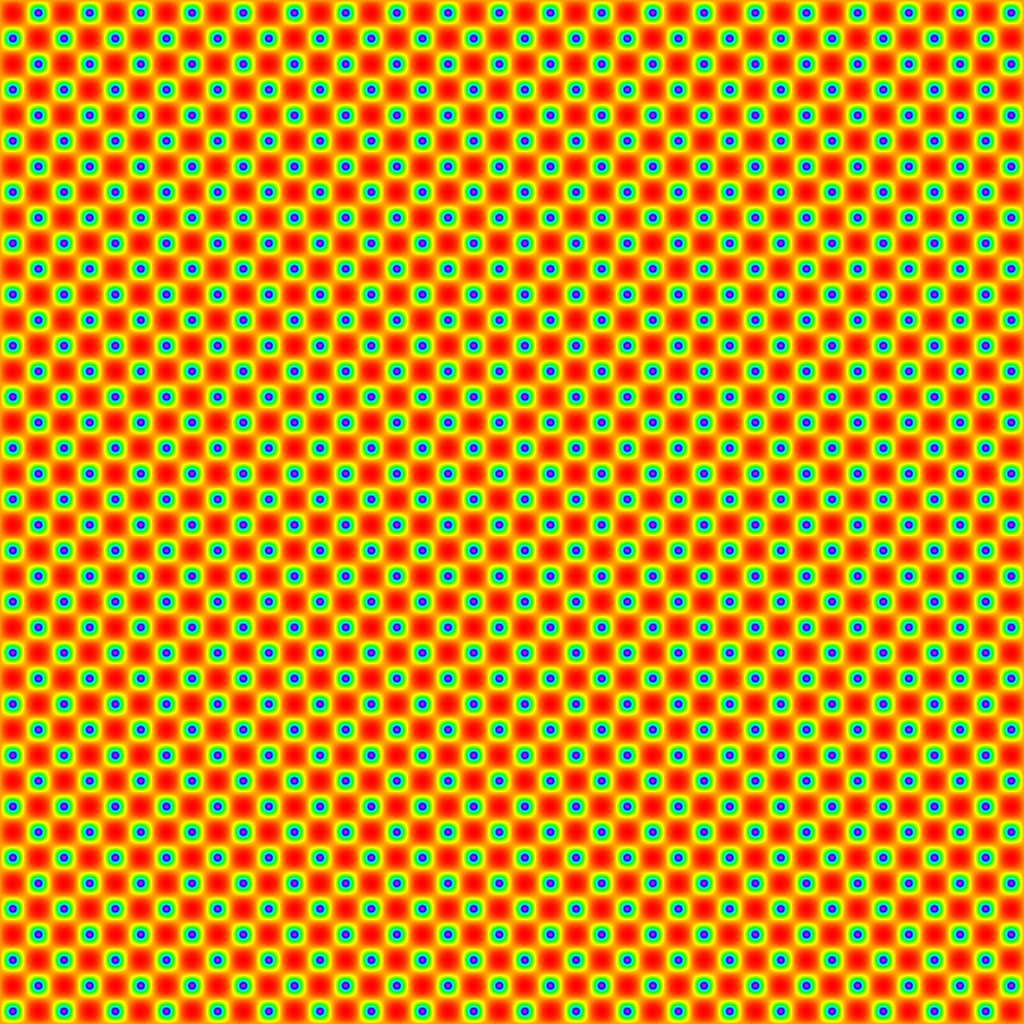
\includegraphics[width=\textwidth]{Figures/speed_sin_checkerboard_s}
		\caption{Sin Checkerboard: $[0.5715, 4]$}
	\end{subfigure}
	\begin{subfigure}[b]{.4\columnwidth}
		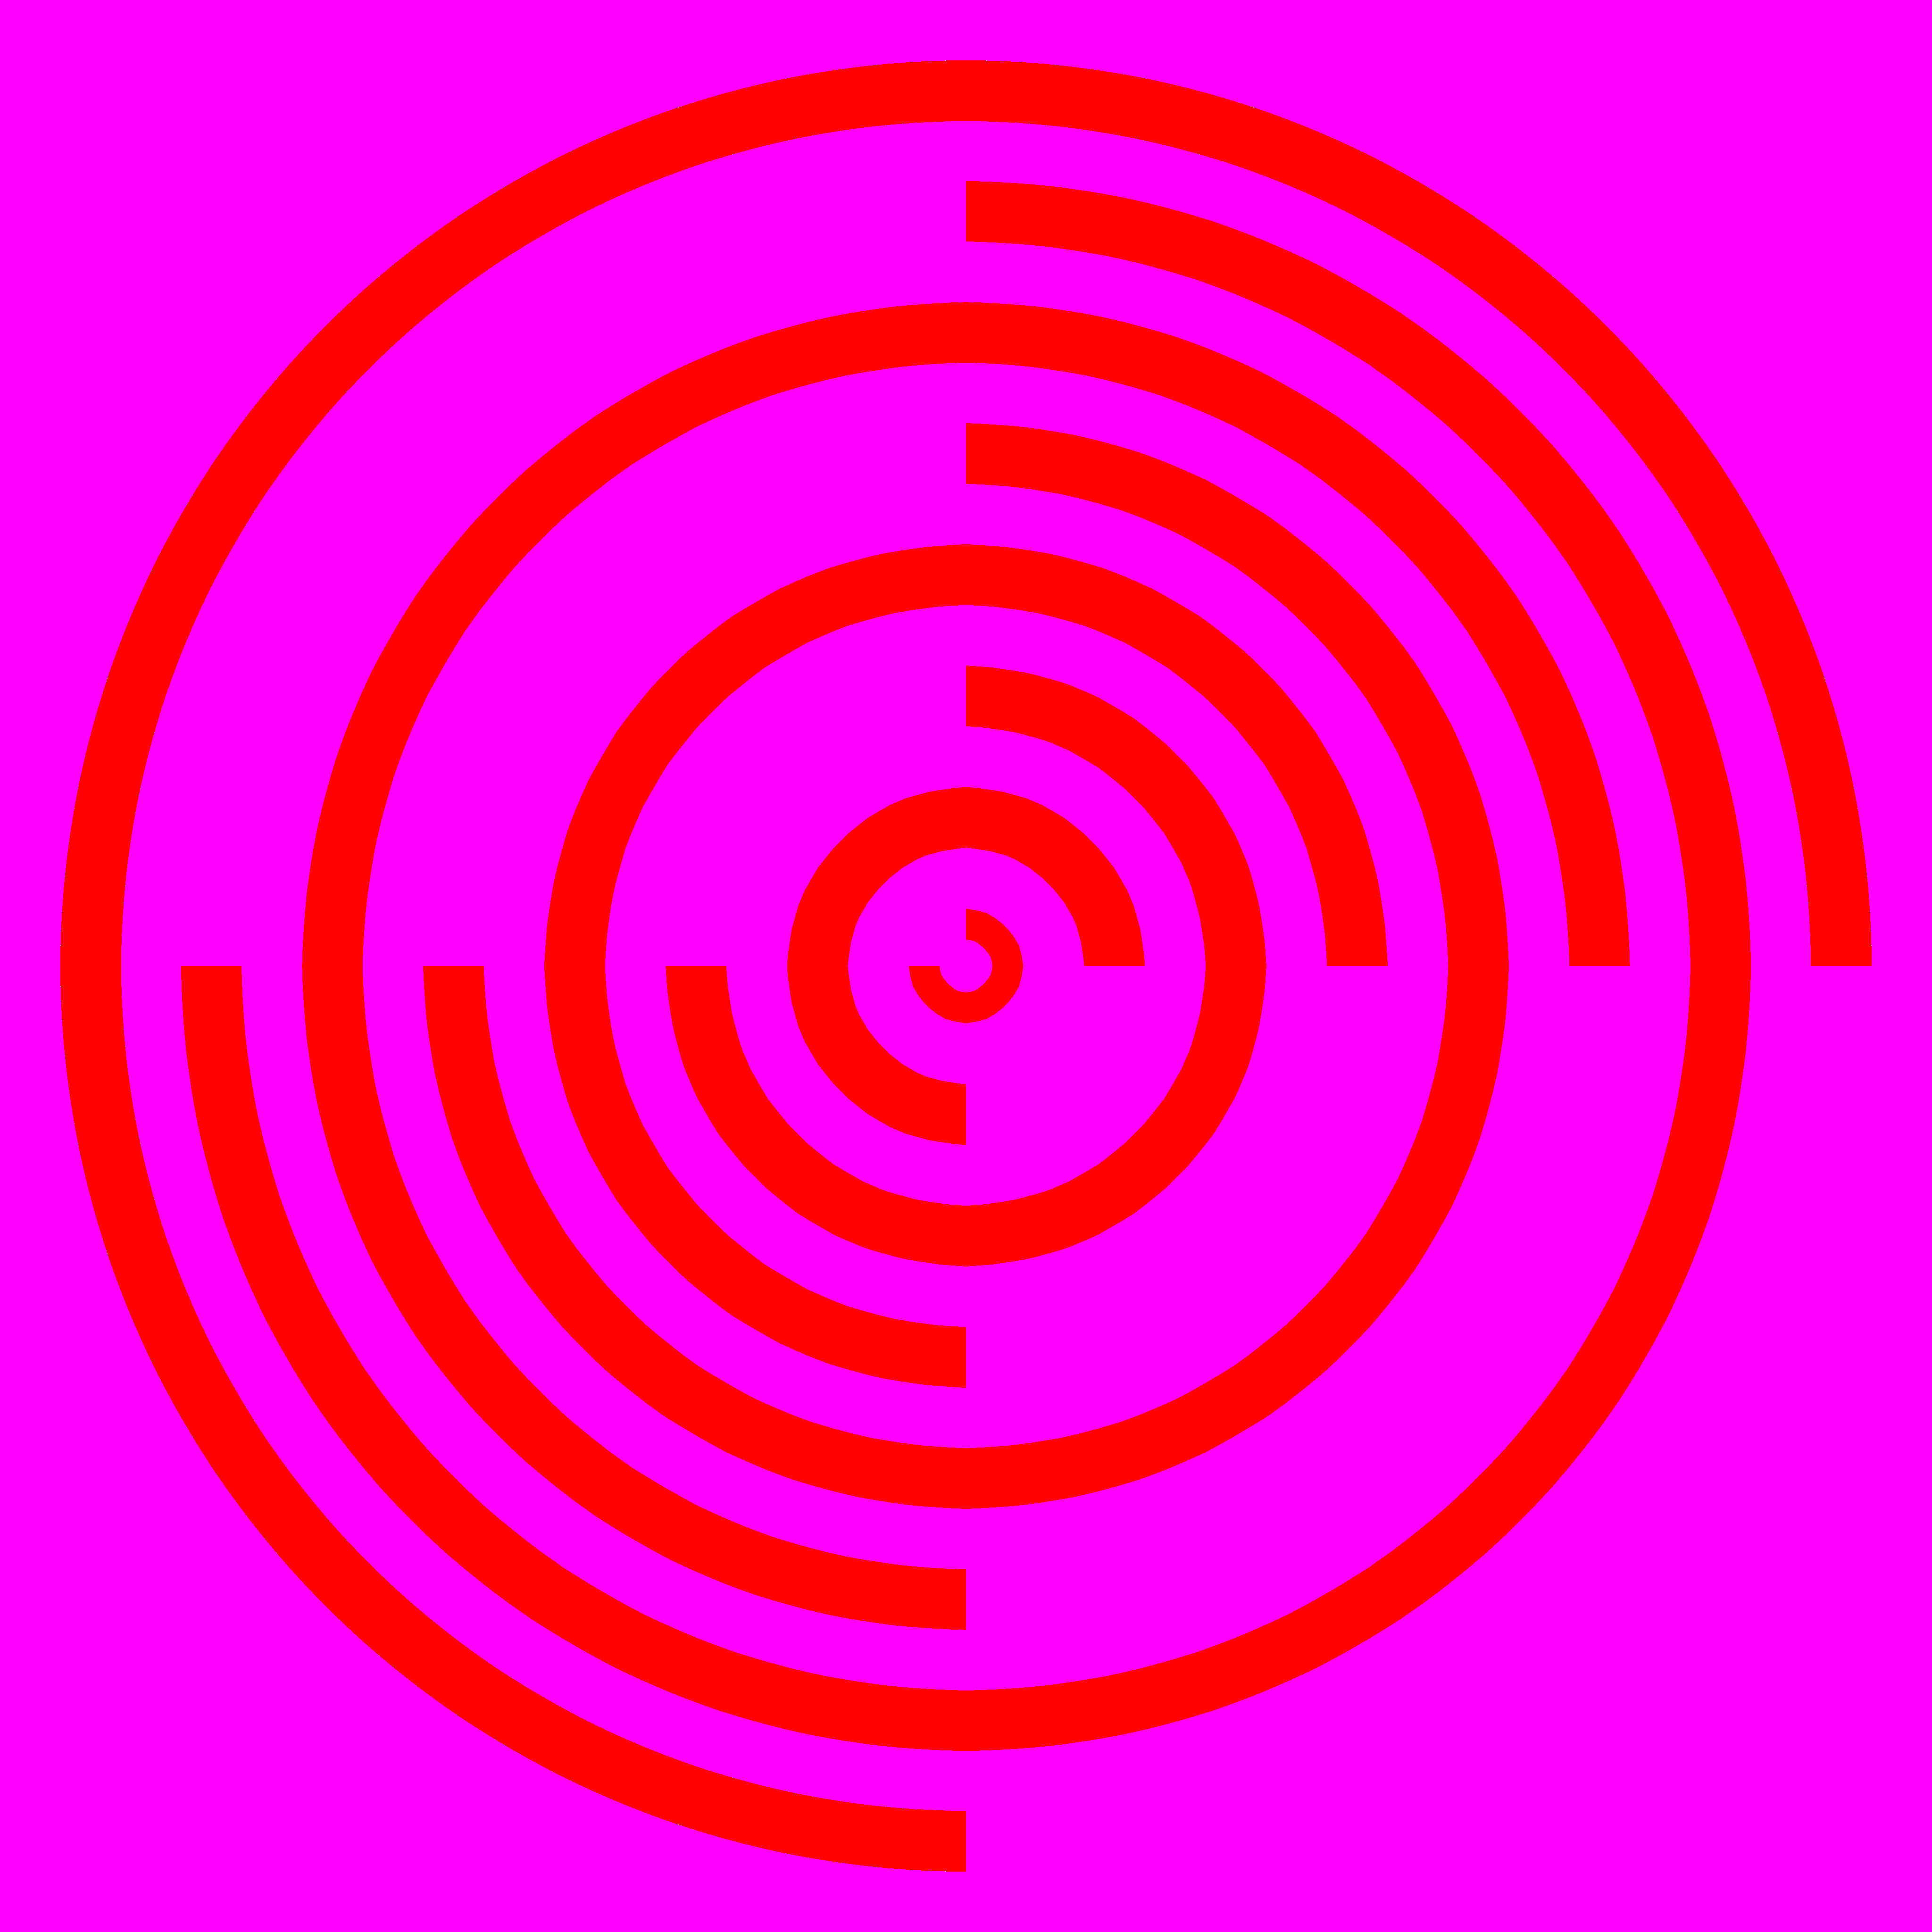
\includegraphics[width=\textwidth]{Figures/speed_7_rings}
		\caption{7-Ring: $[0, 1]$}
	\end{subfigure}
	\begin{subfigure}[b]{.4\columnwidth}
		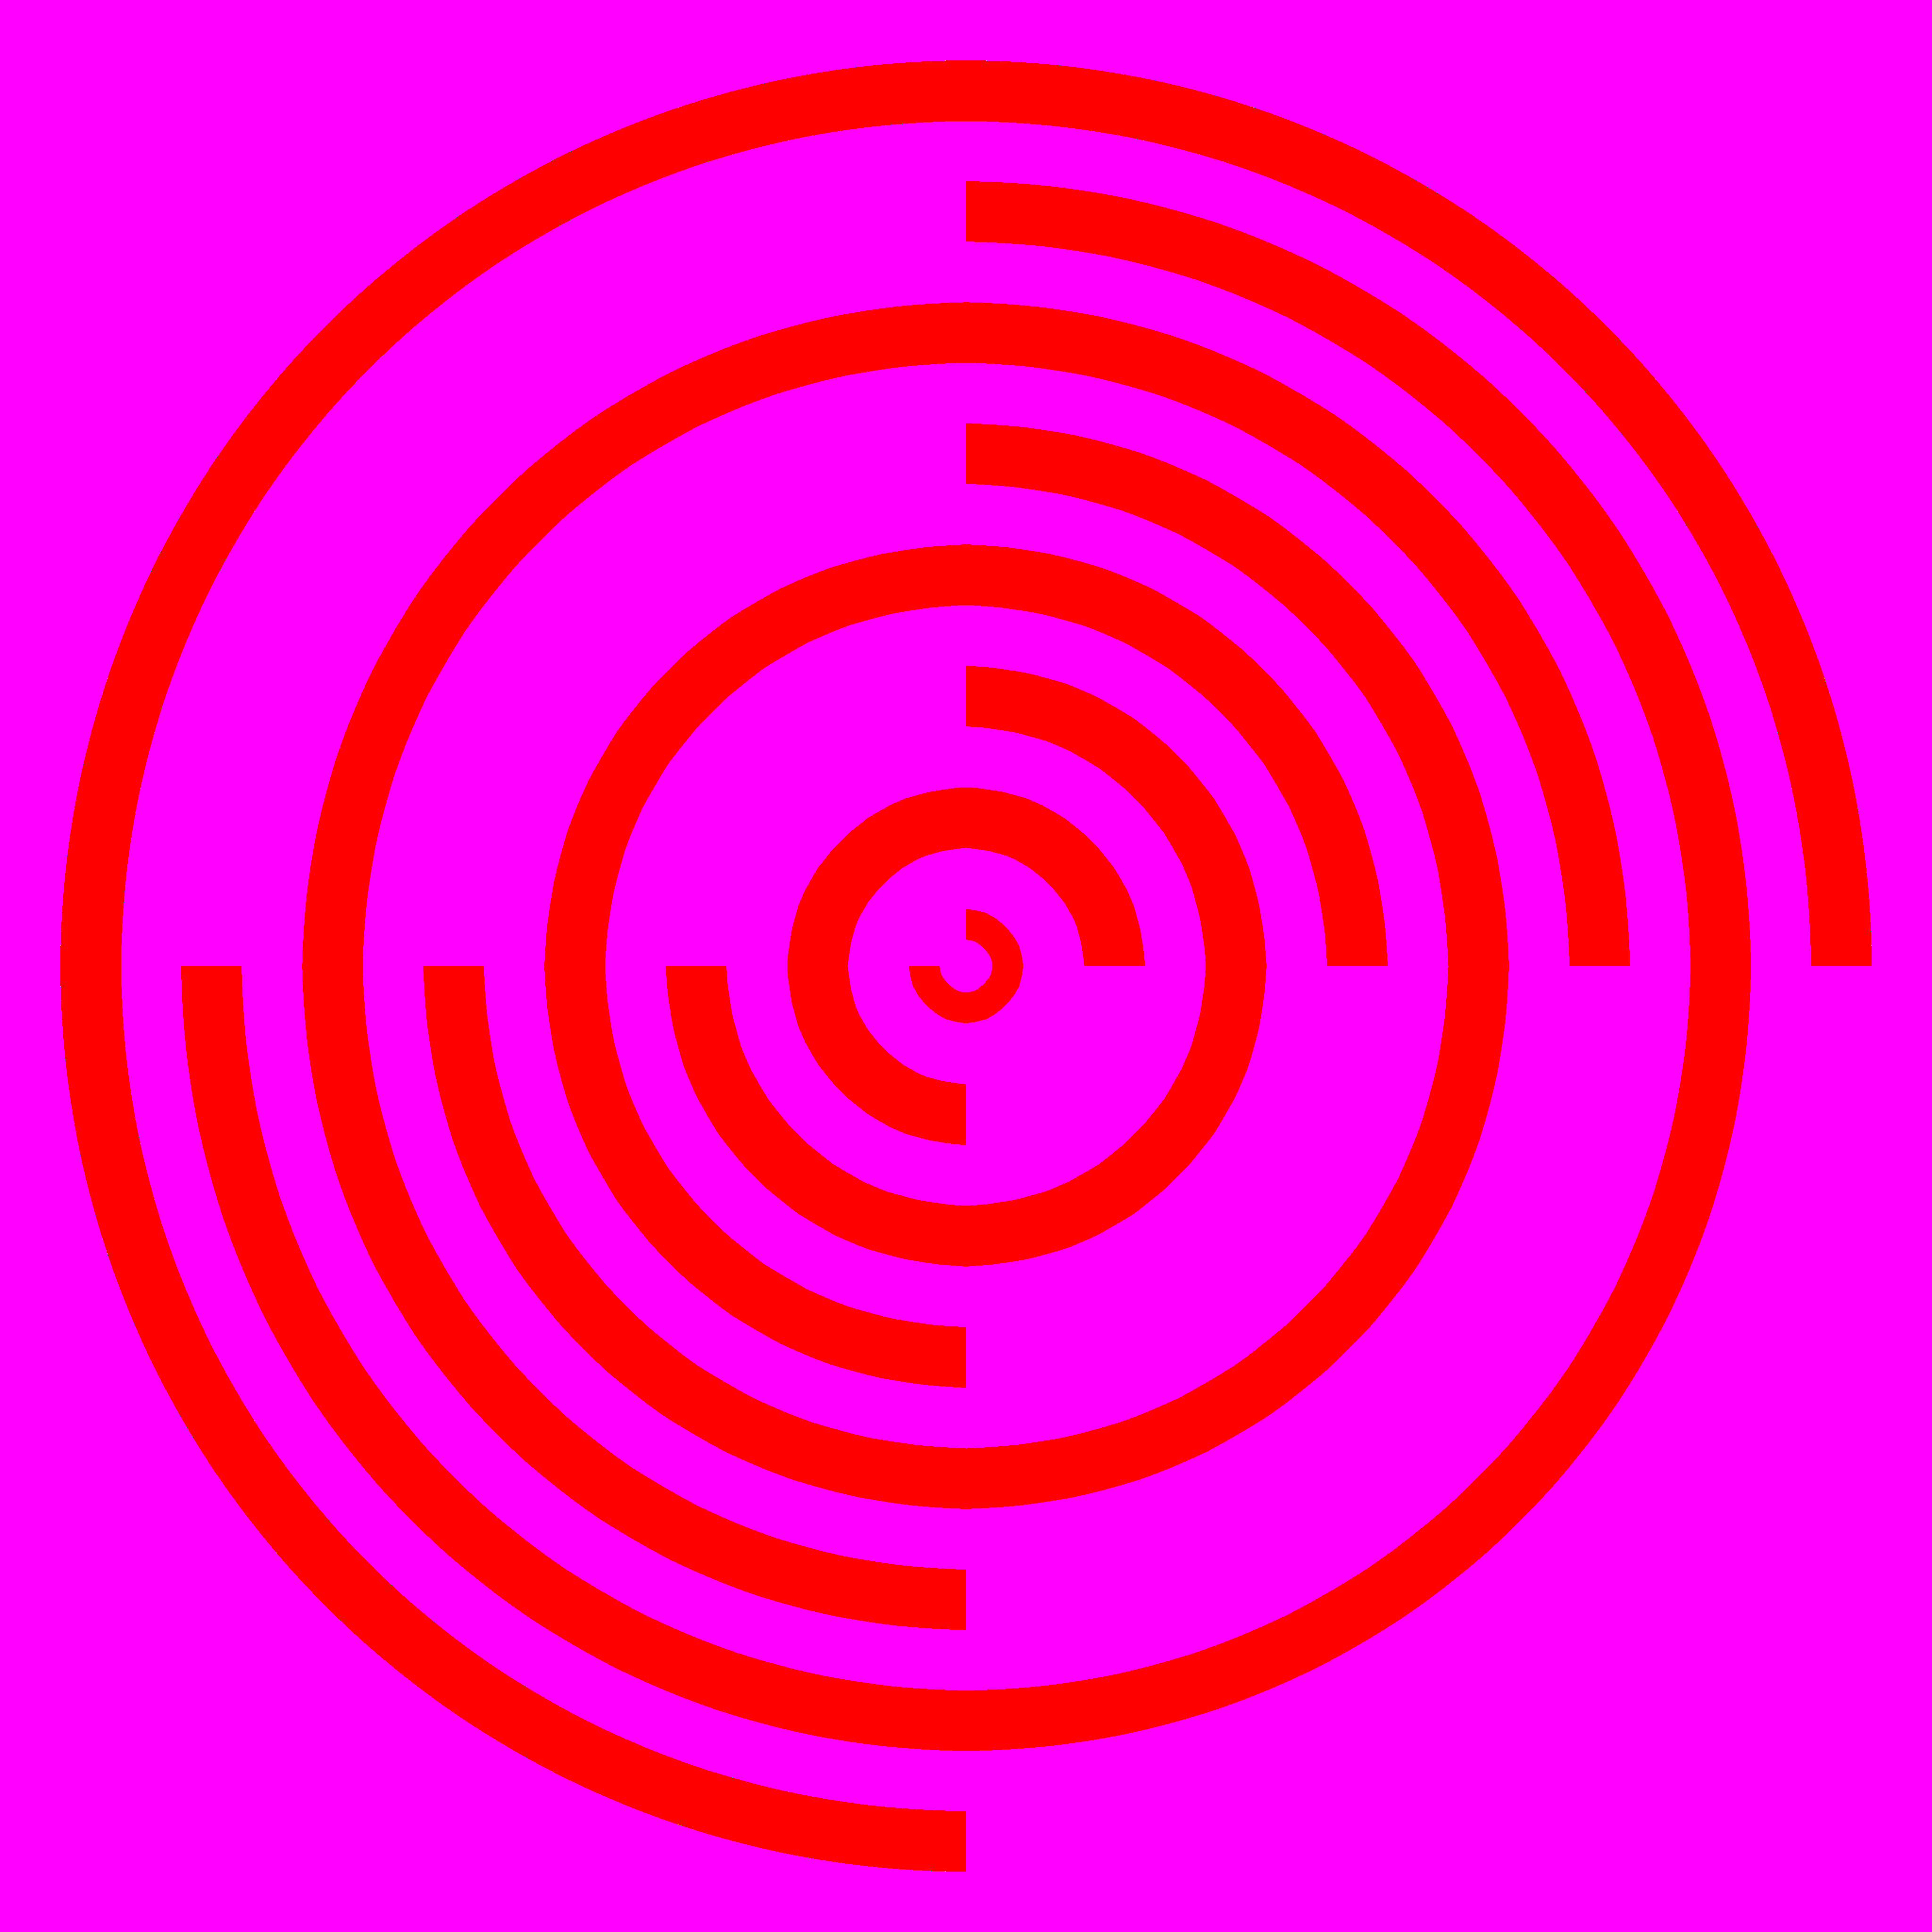
\includegraphics[width=\textwidth]{Figures/speed_7_rings_permeable}
		\caption{7-Ring Permeable: $[0.001, 1]$}
	\end{subfigure}
	\begin{subfigure}[b]{.4\columnwidth}
		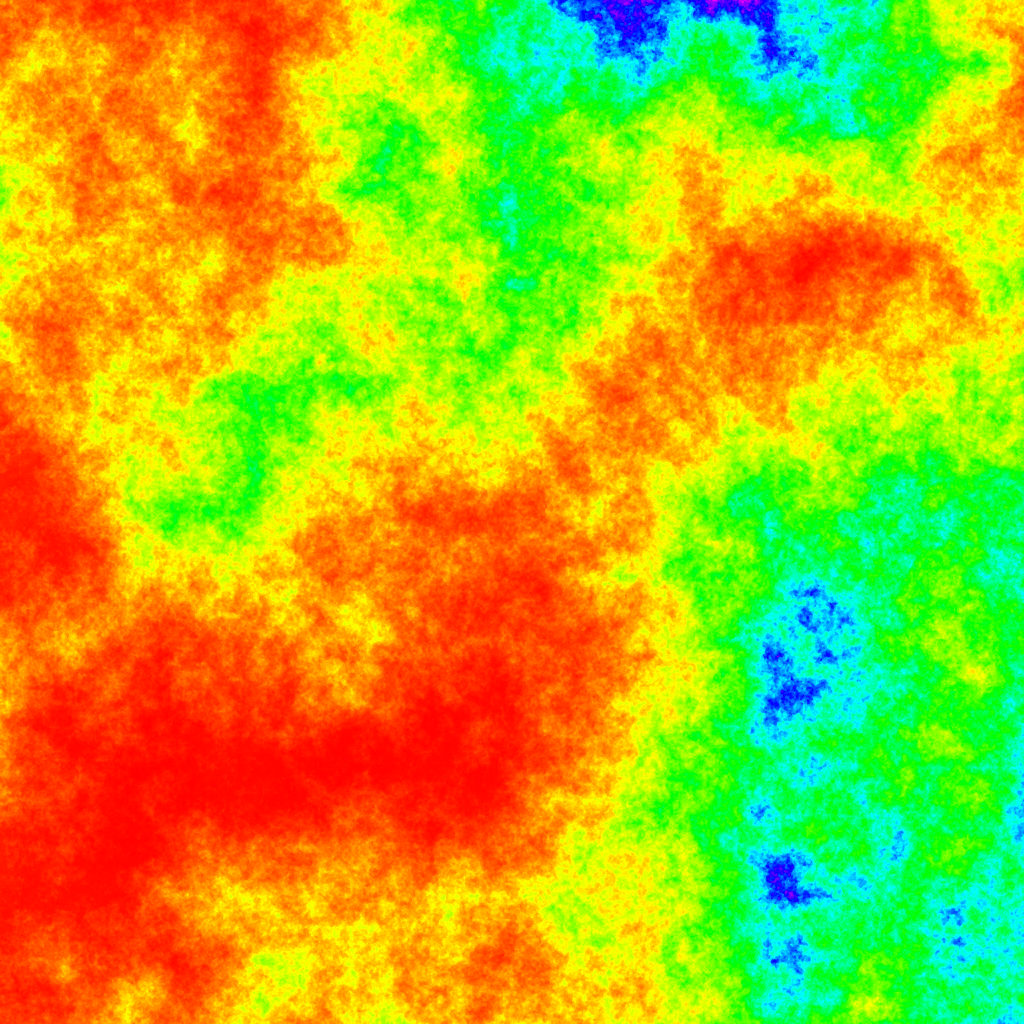
\includegraphics[width=\textwidth]{Figures/speed_cloudy_s}
		\caption{Cloudy: $[0.005, 0.789]$}
	\end{subfigure}
	\begin{subfigure}[b]{.4\columnwidth}
		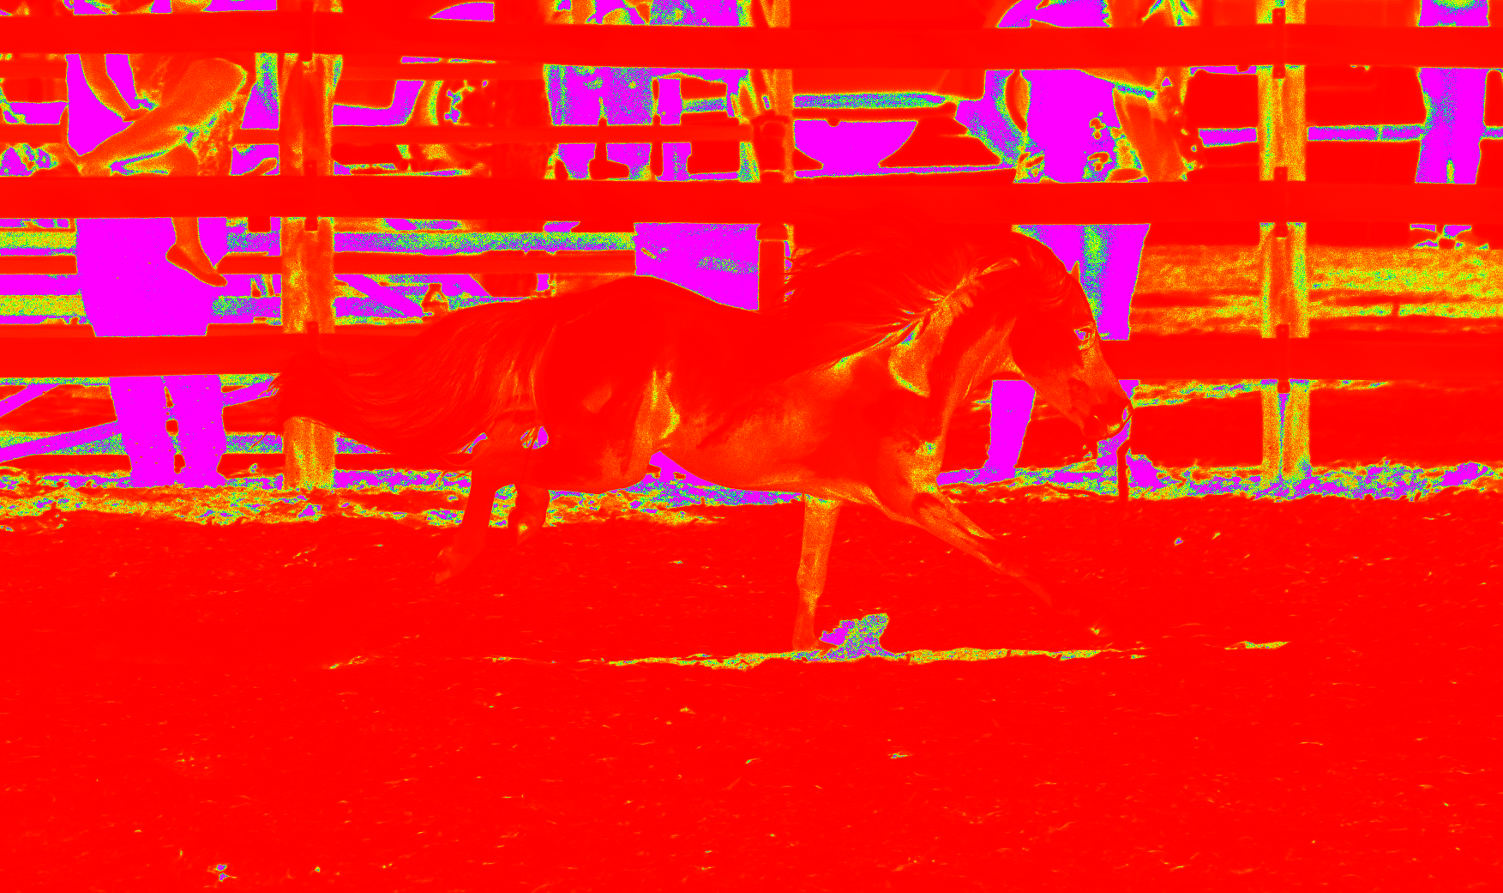
\includegraphics[width=\textwidth]{Figures/speed_photograph_s}
		\caption{Photograph: $[1, 10000]$}
	\end{subfigure}
	\caption{$f(x)$ fields for each test case. Hue'd from Red (lower bound) to Magenta (upper bound).}
	\label{fig:speed_field}
\end{figure}

\begin{figure}%[!b]
	\centering
	\begin{subfigure}[b]{.3\columnwidth}
		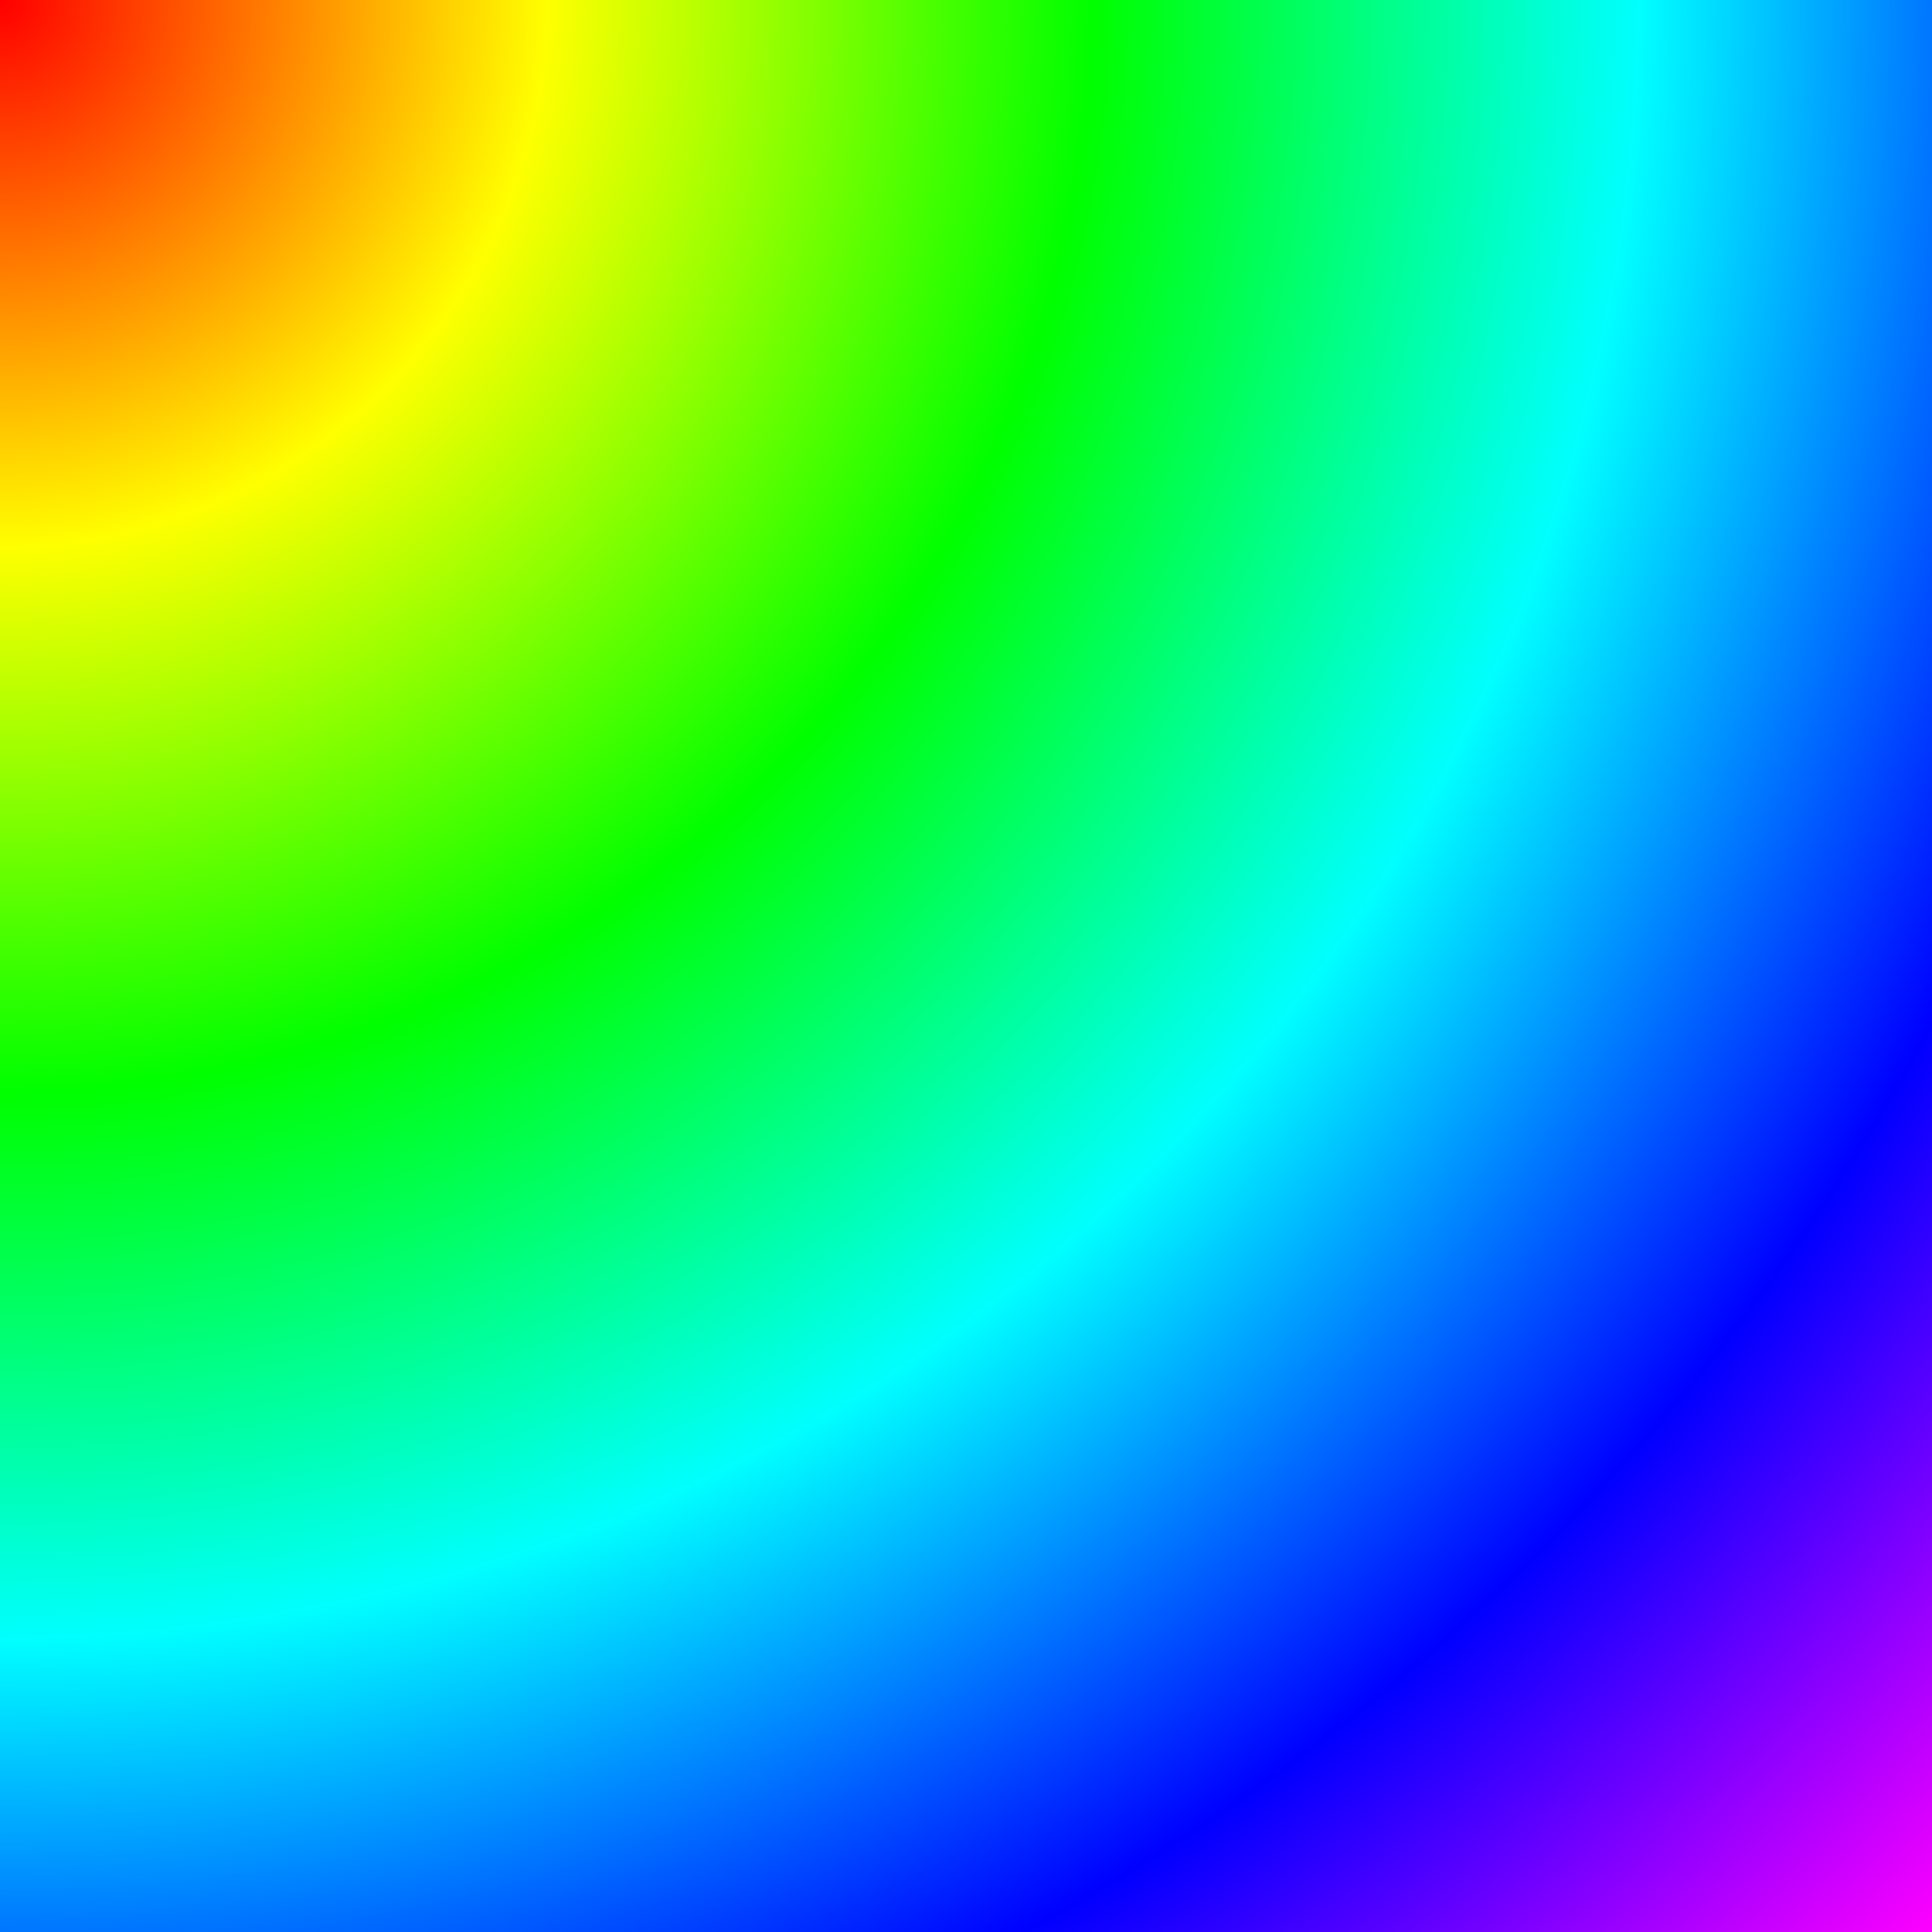
\includegraphics[width=\textwidth]{Figures/fmm_constant}
	\end{subfigure}
	\begin{subfigure}[b]{.3\columnwidth}
		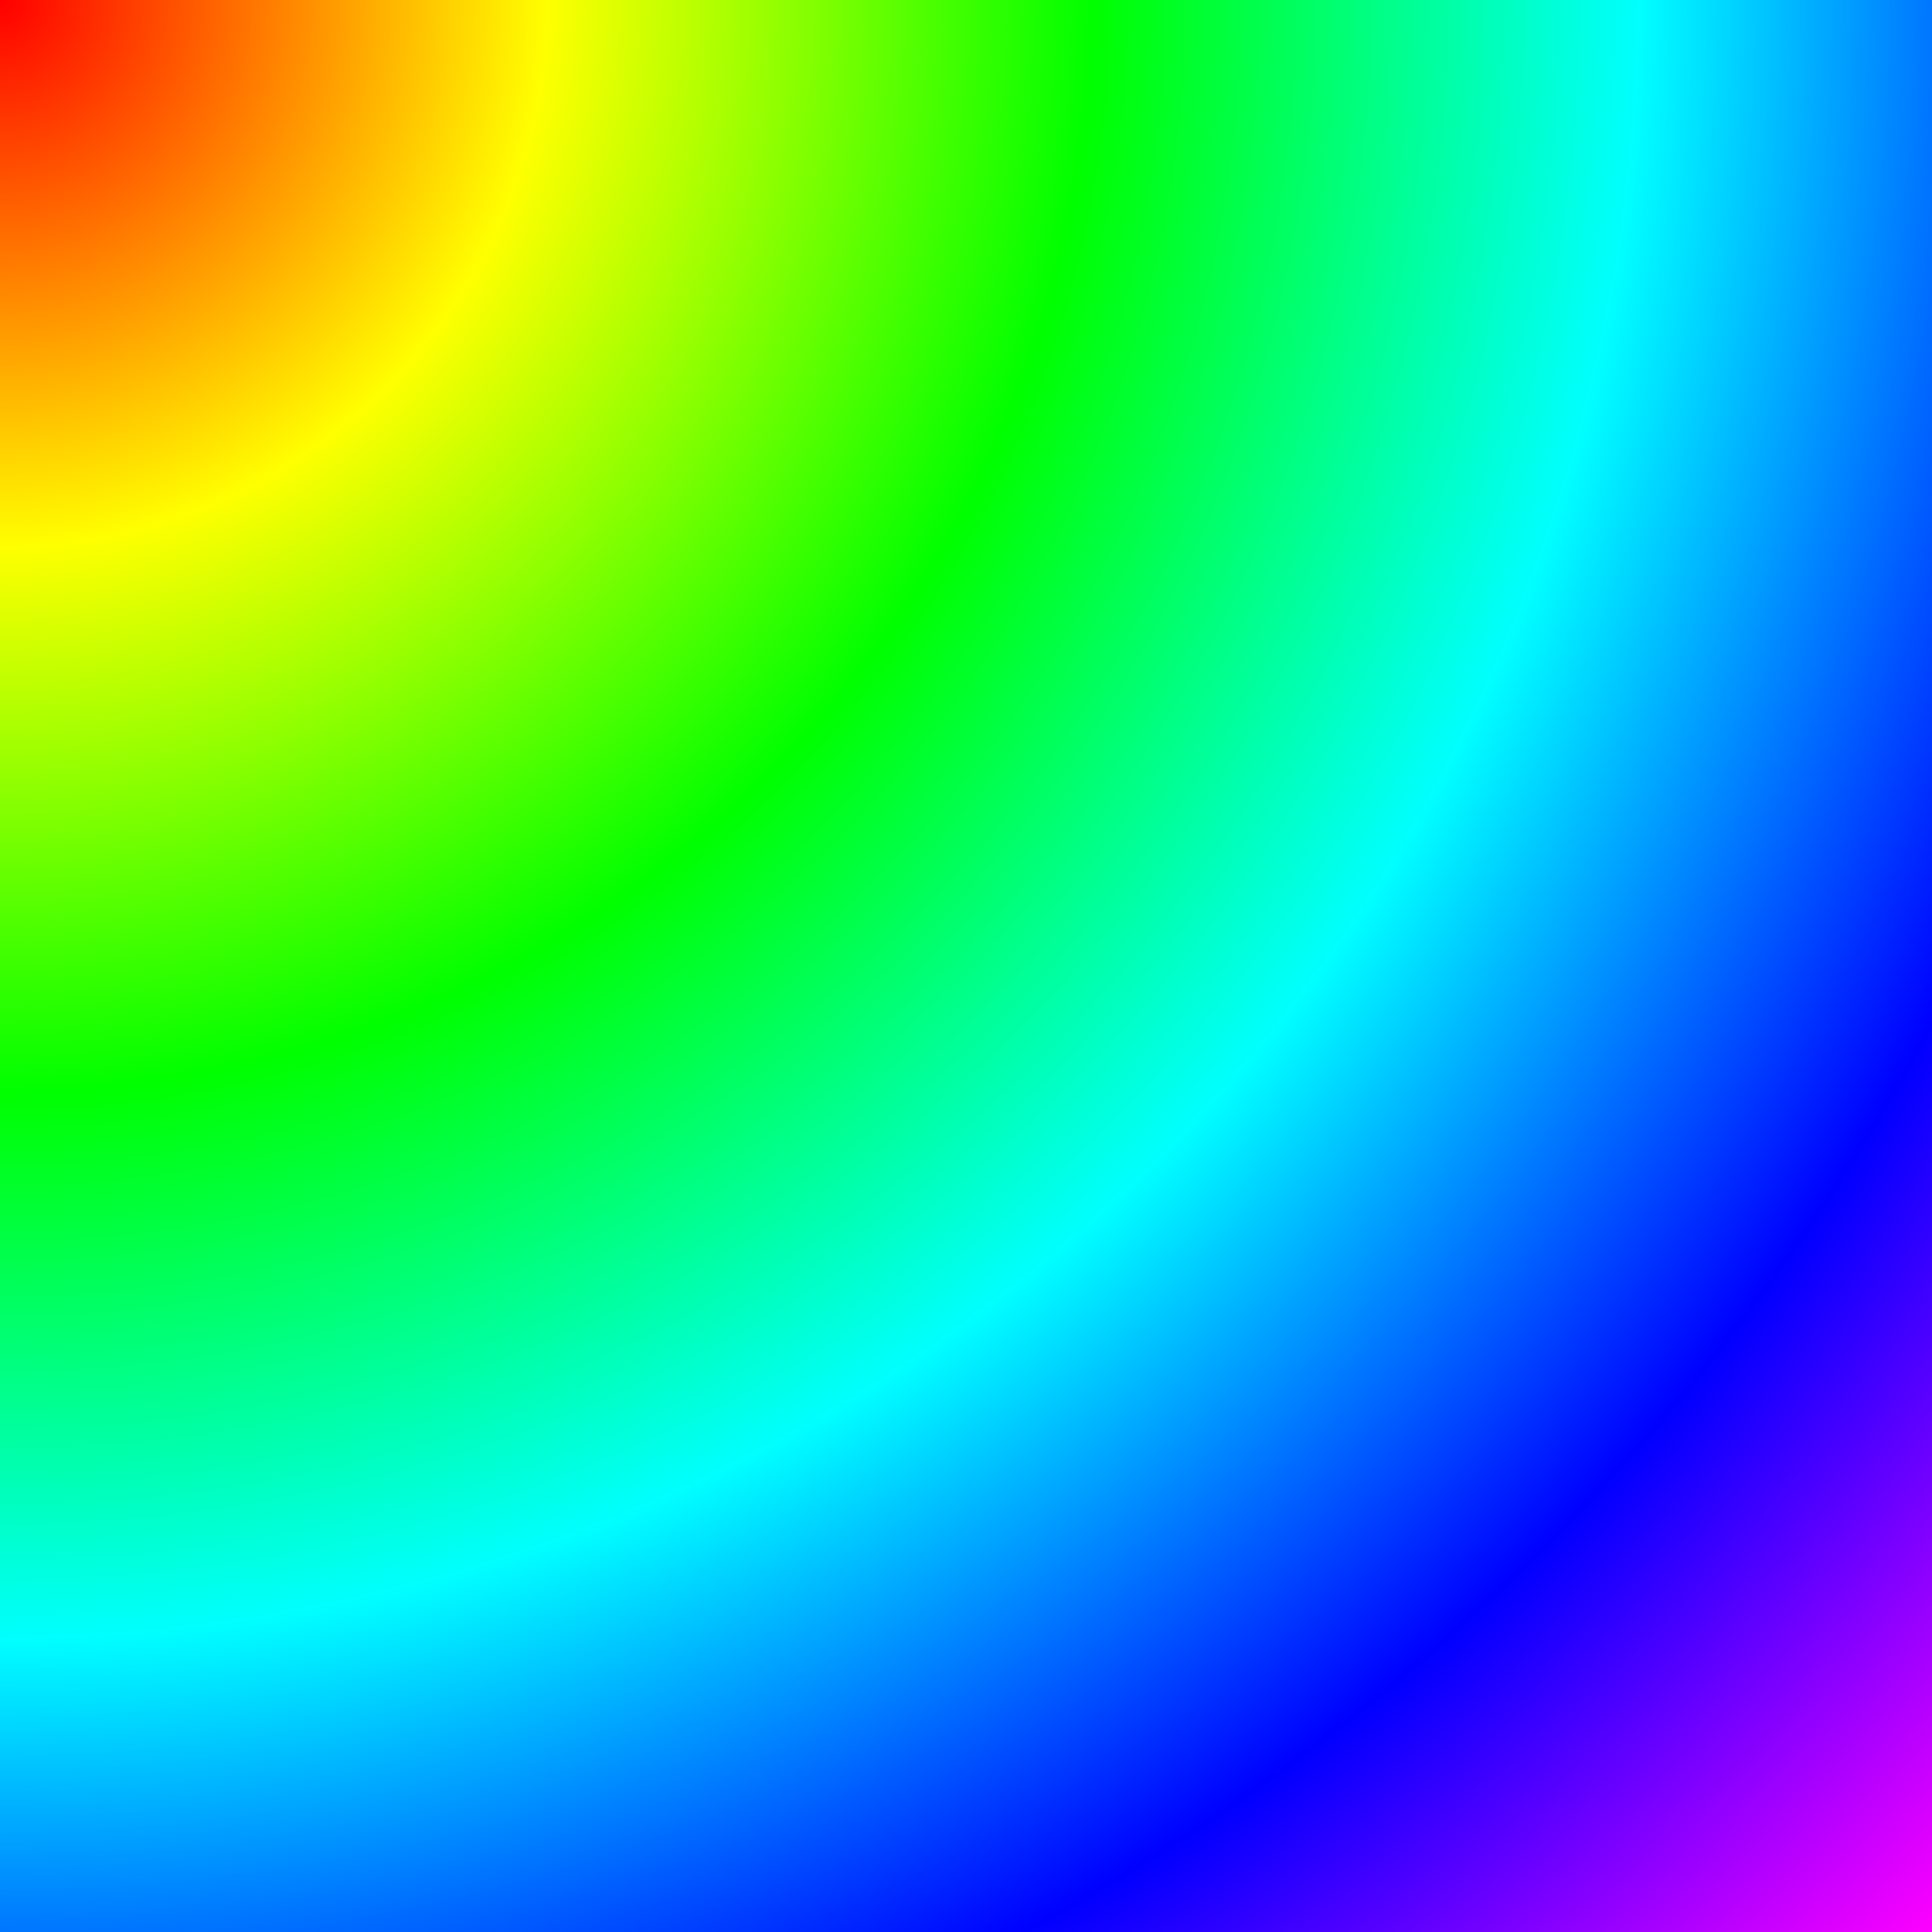
\includegraphics[width=\textwidth]{Figures/fim_constant}
	\end{subfigure}
	\begin{subfigure}[b]{.3\columnwidth}
		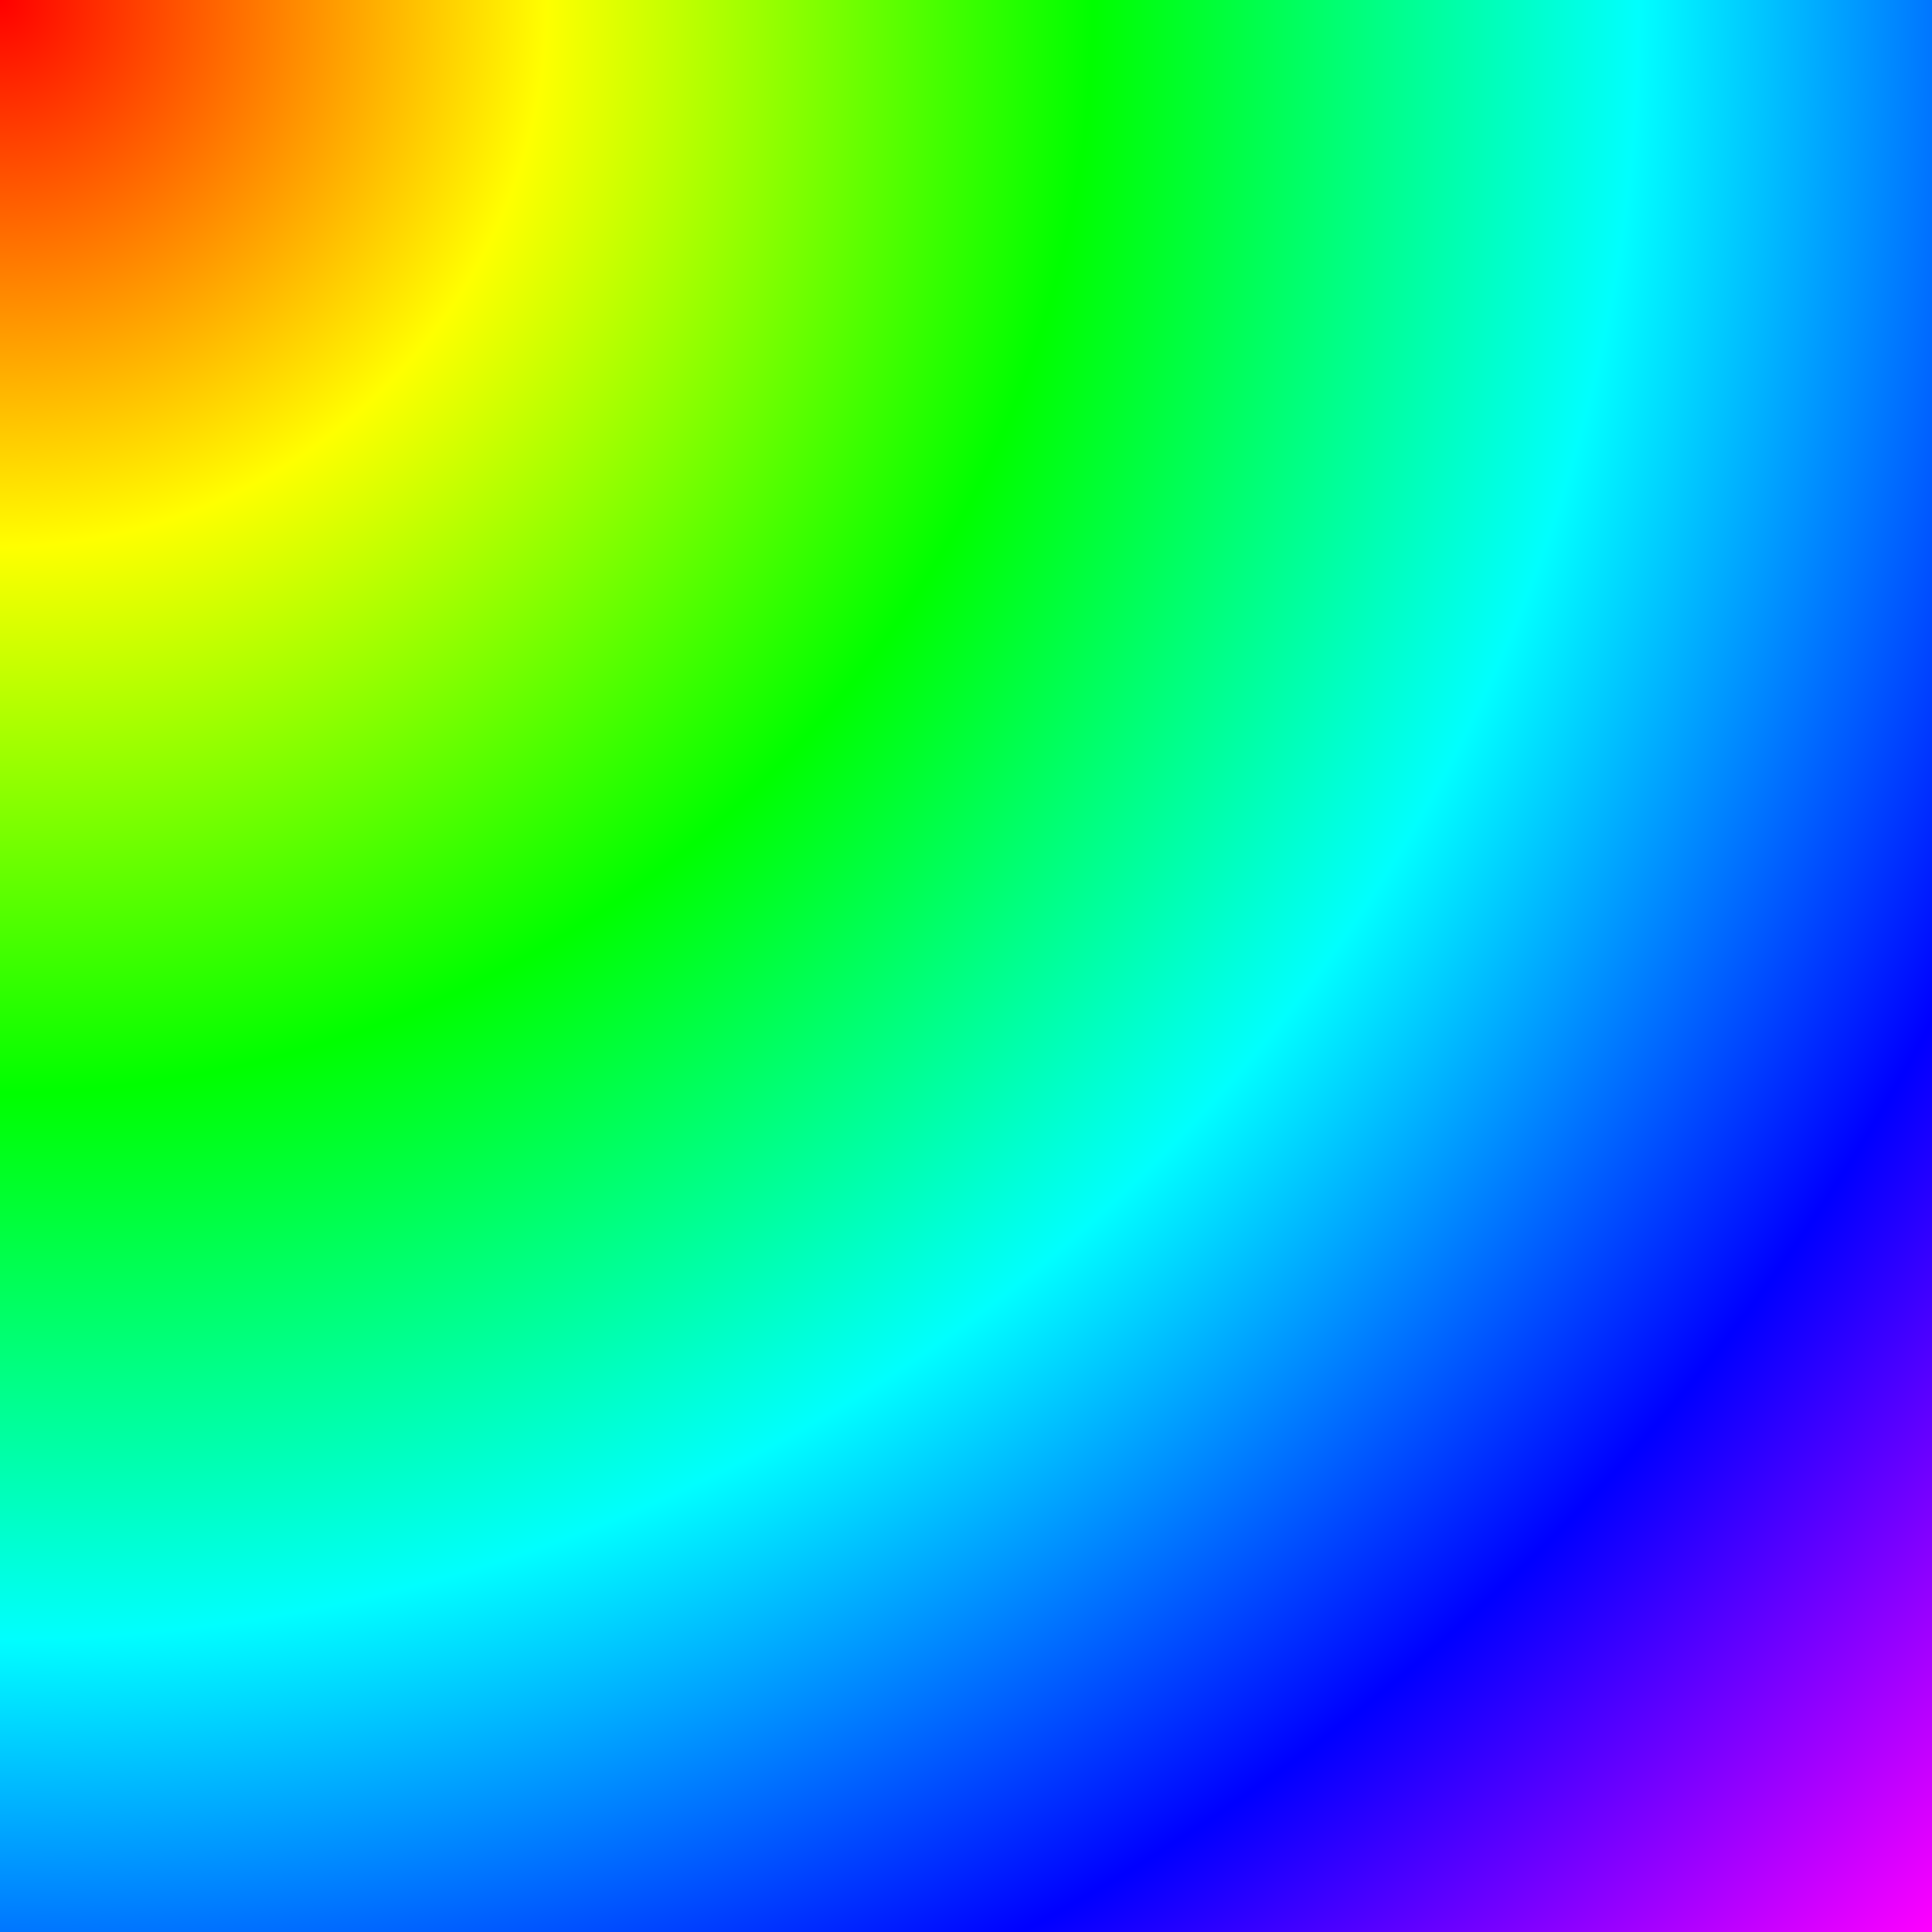
\includegraphics[width=\textwidth]{Figures/ghcm_systolic_constant}
	\end{subfigure}
	
	\begin{subfigure}[b]{.3\columnwidth}
		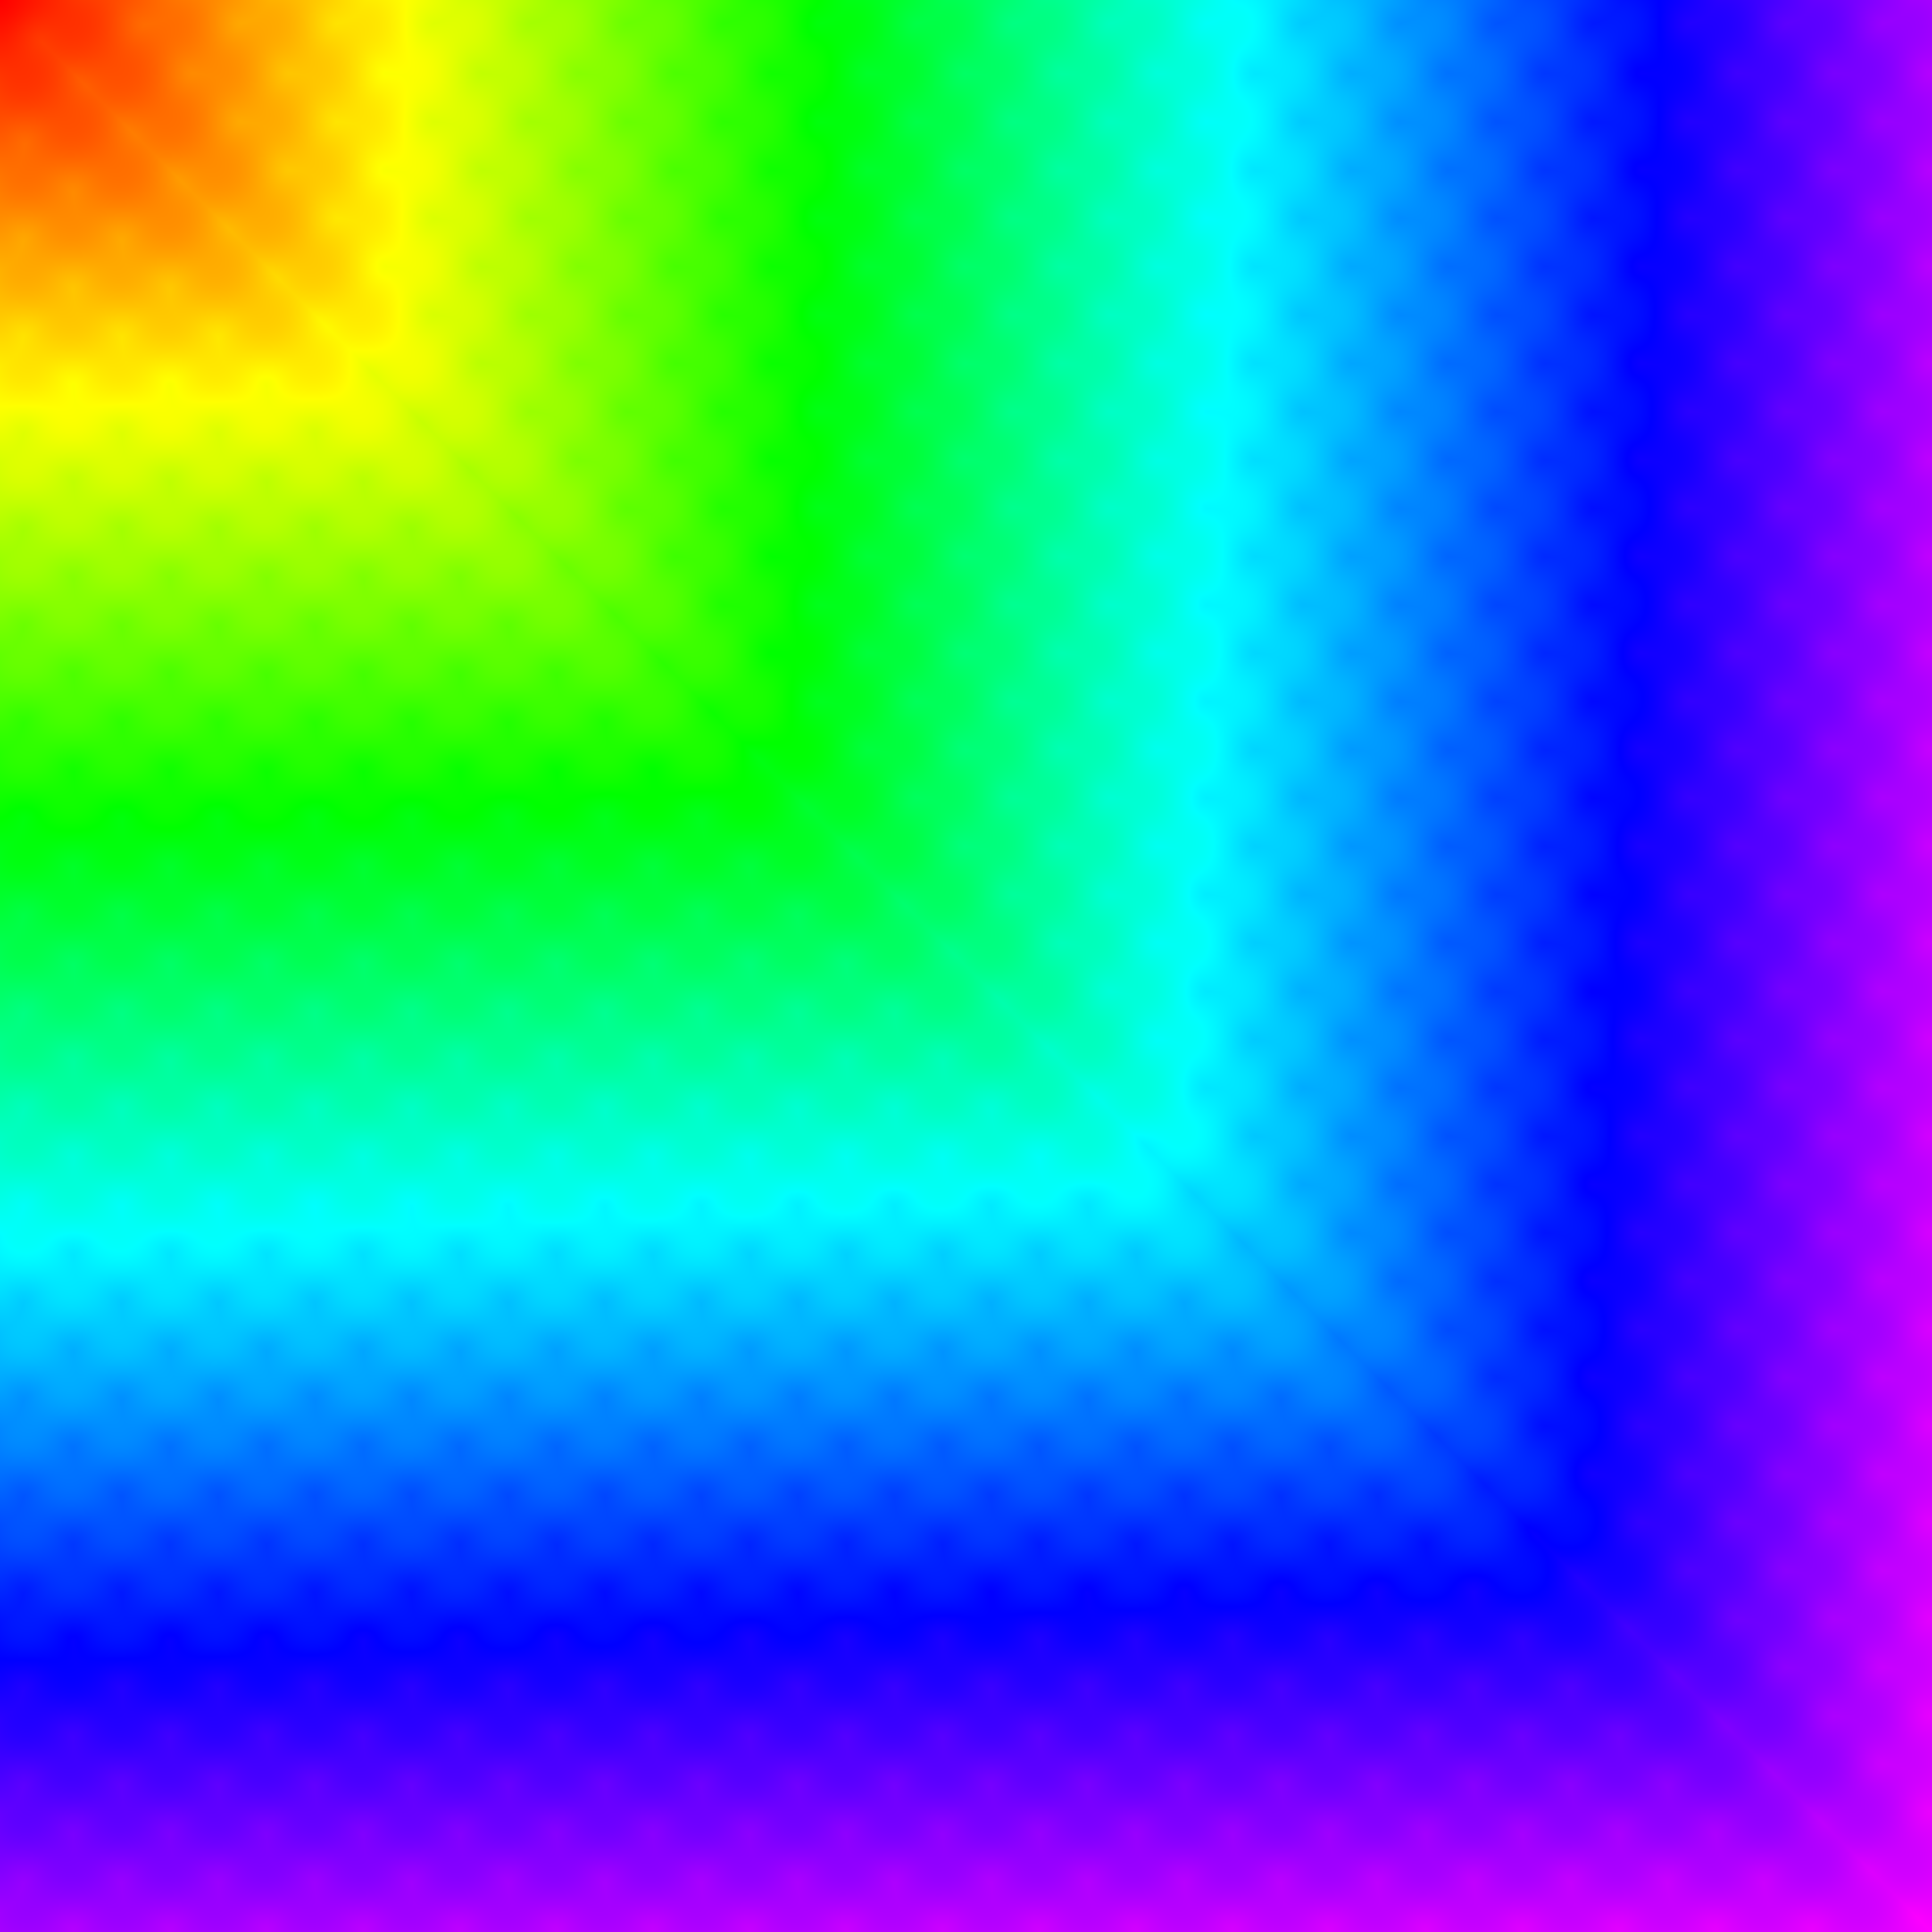
\includegraphics[width=\textwidth]{Figures/fmm_sin_checkerboard}
	\end{subfigure}
	\begin{subfigure}[b]{.3\columnwidth}
		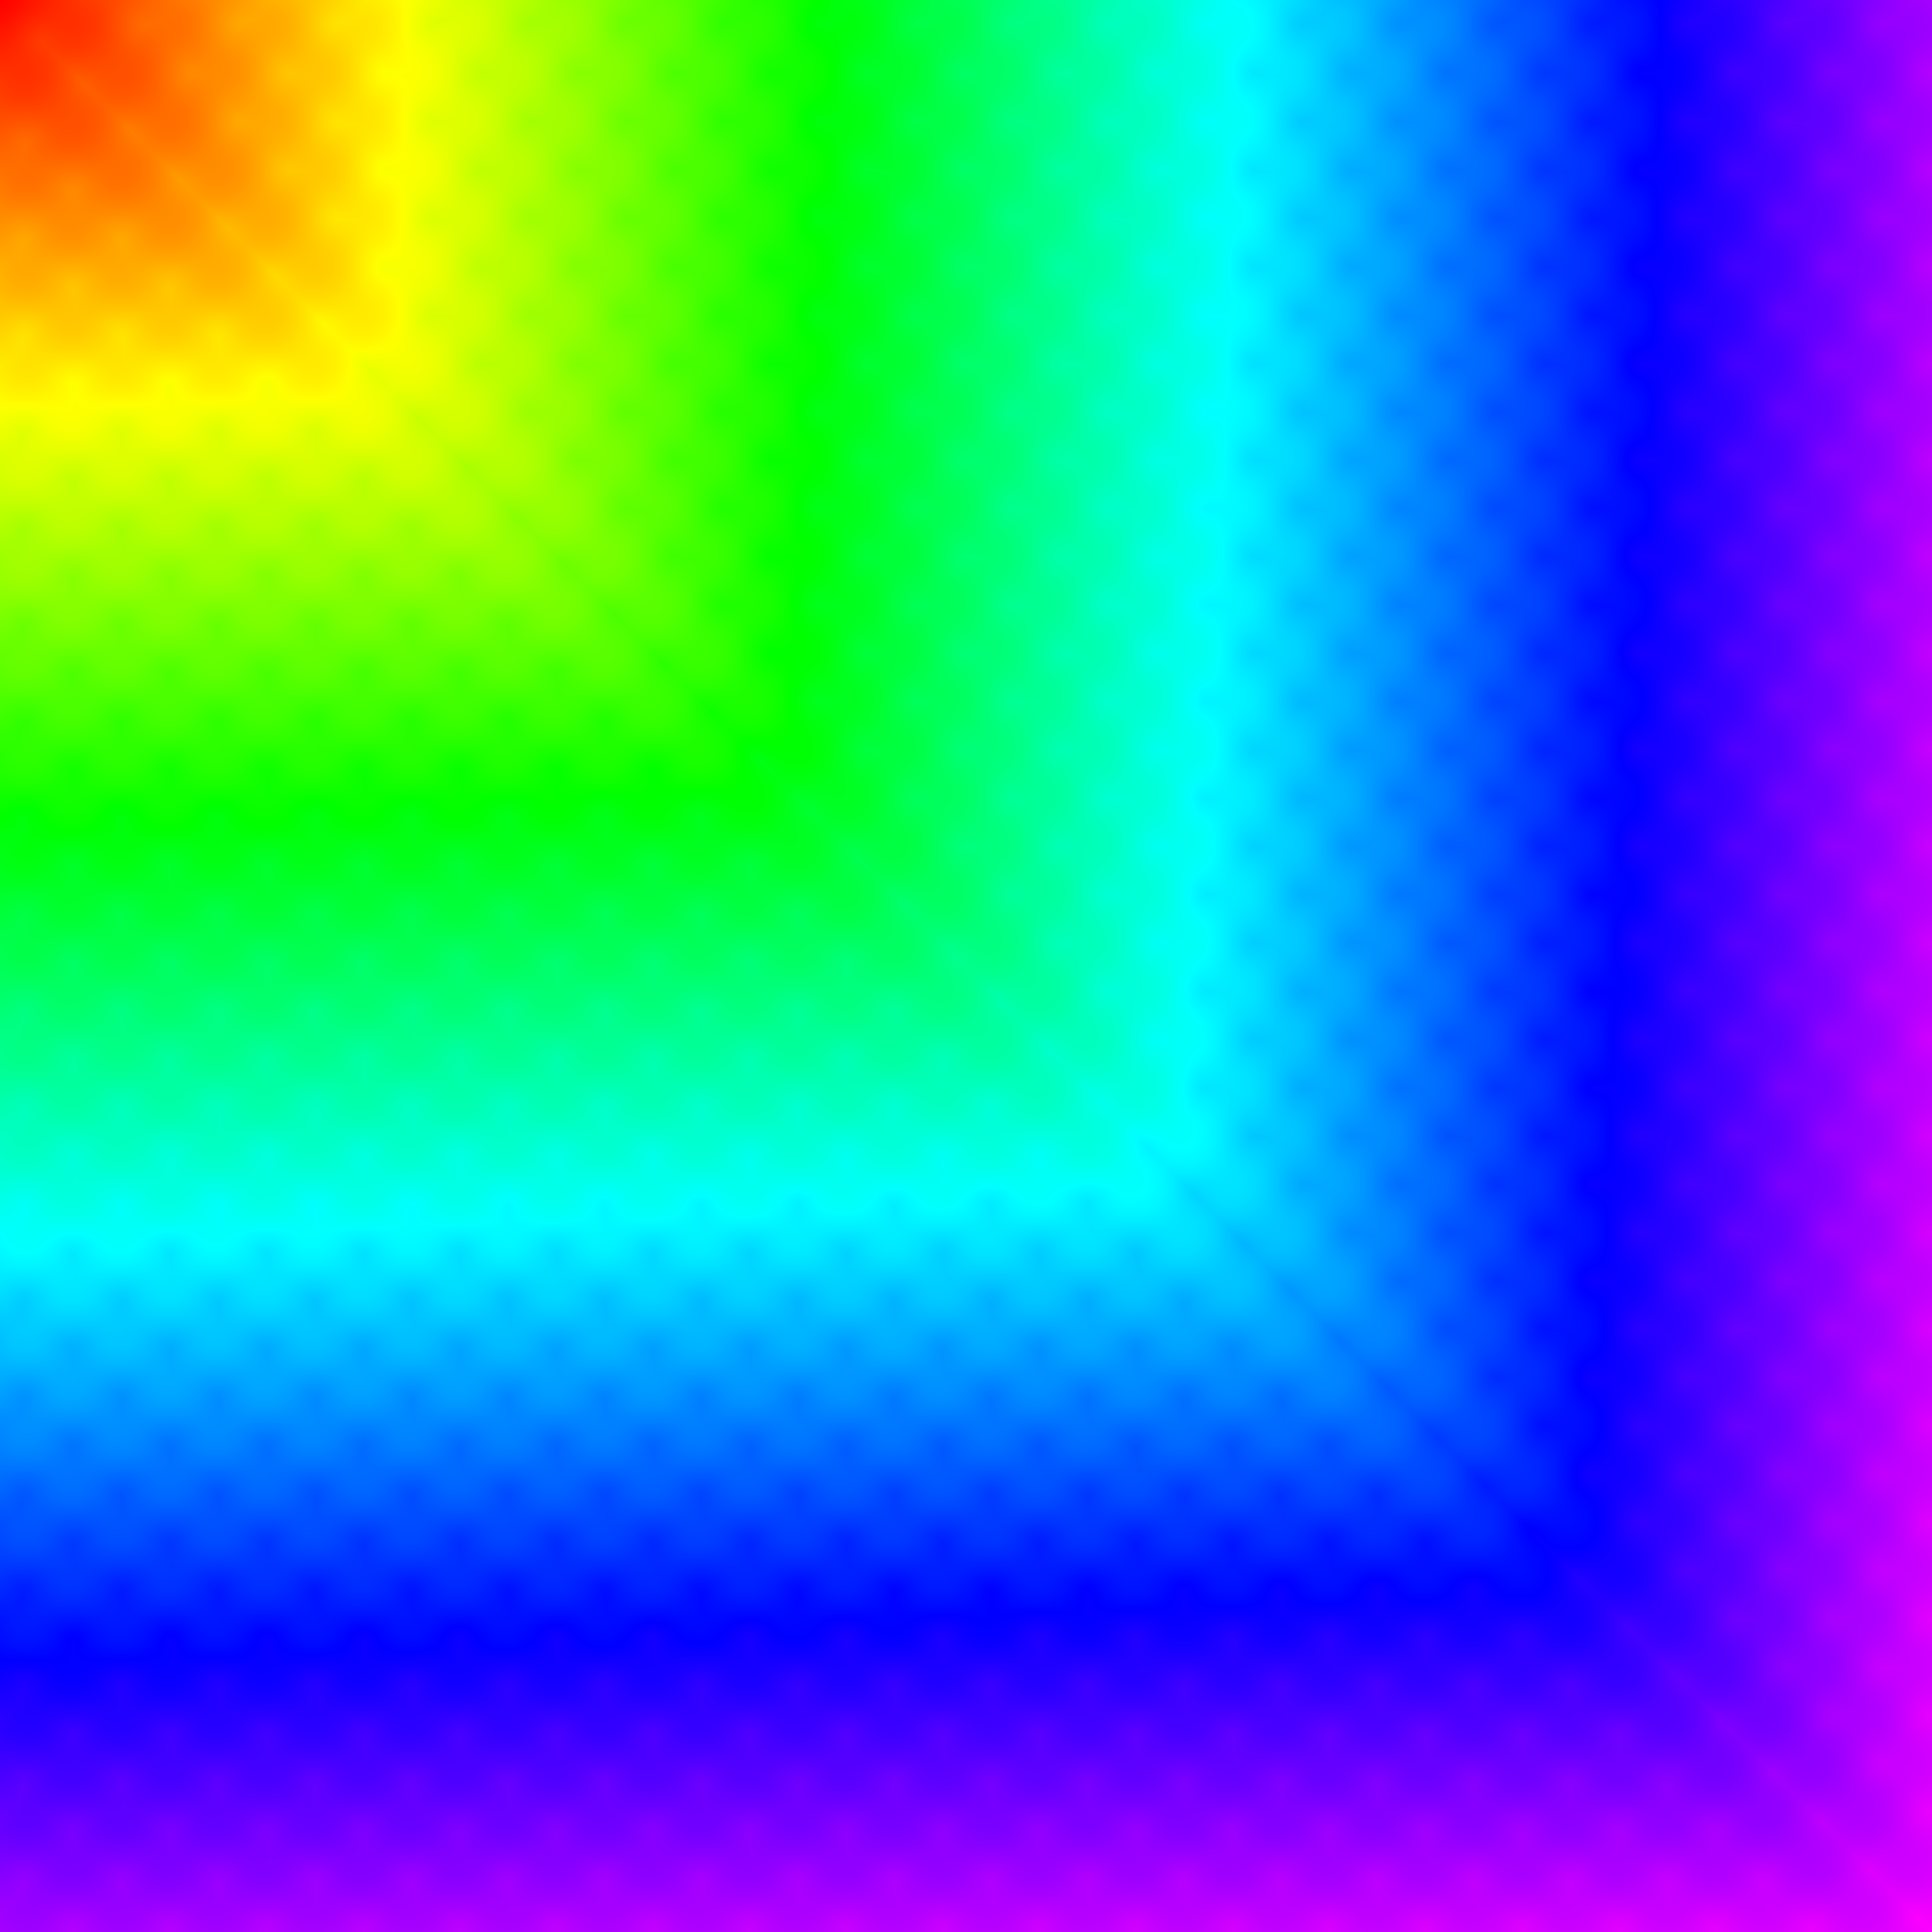
\includegraphics[width=\textwidth]{Figures/fim_sin_checkerboard}
	\end{subfigure}
	\begin{subfigure}[b]{.3\columnwidth}
		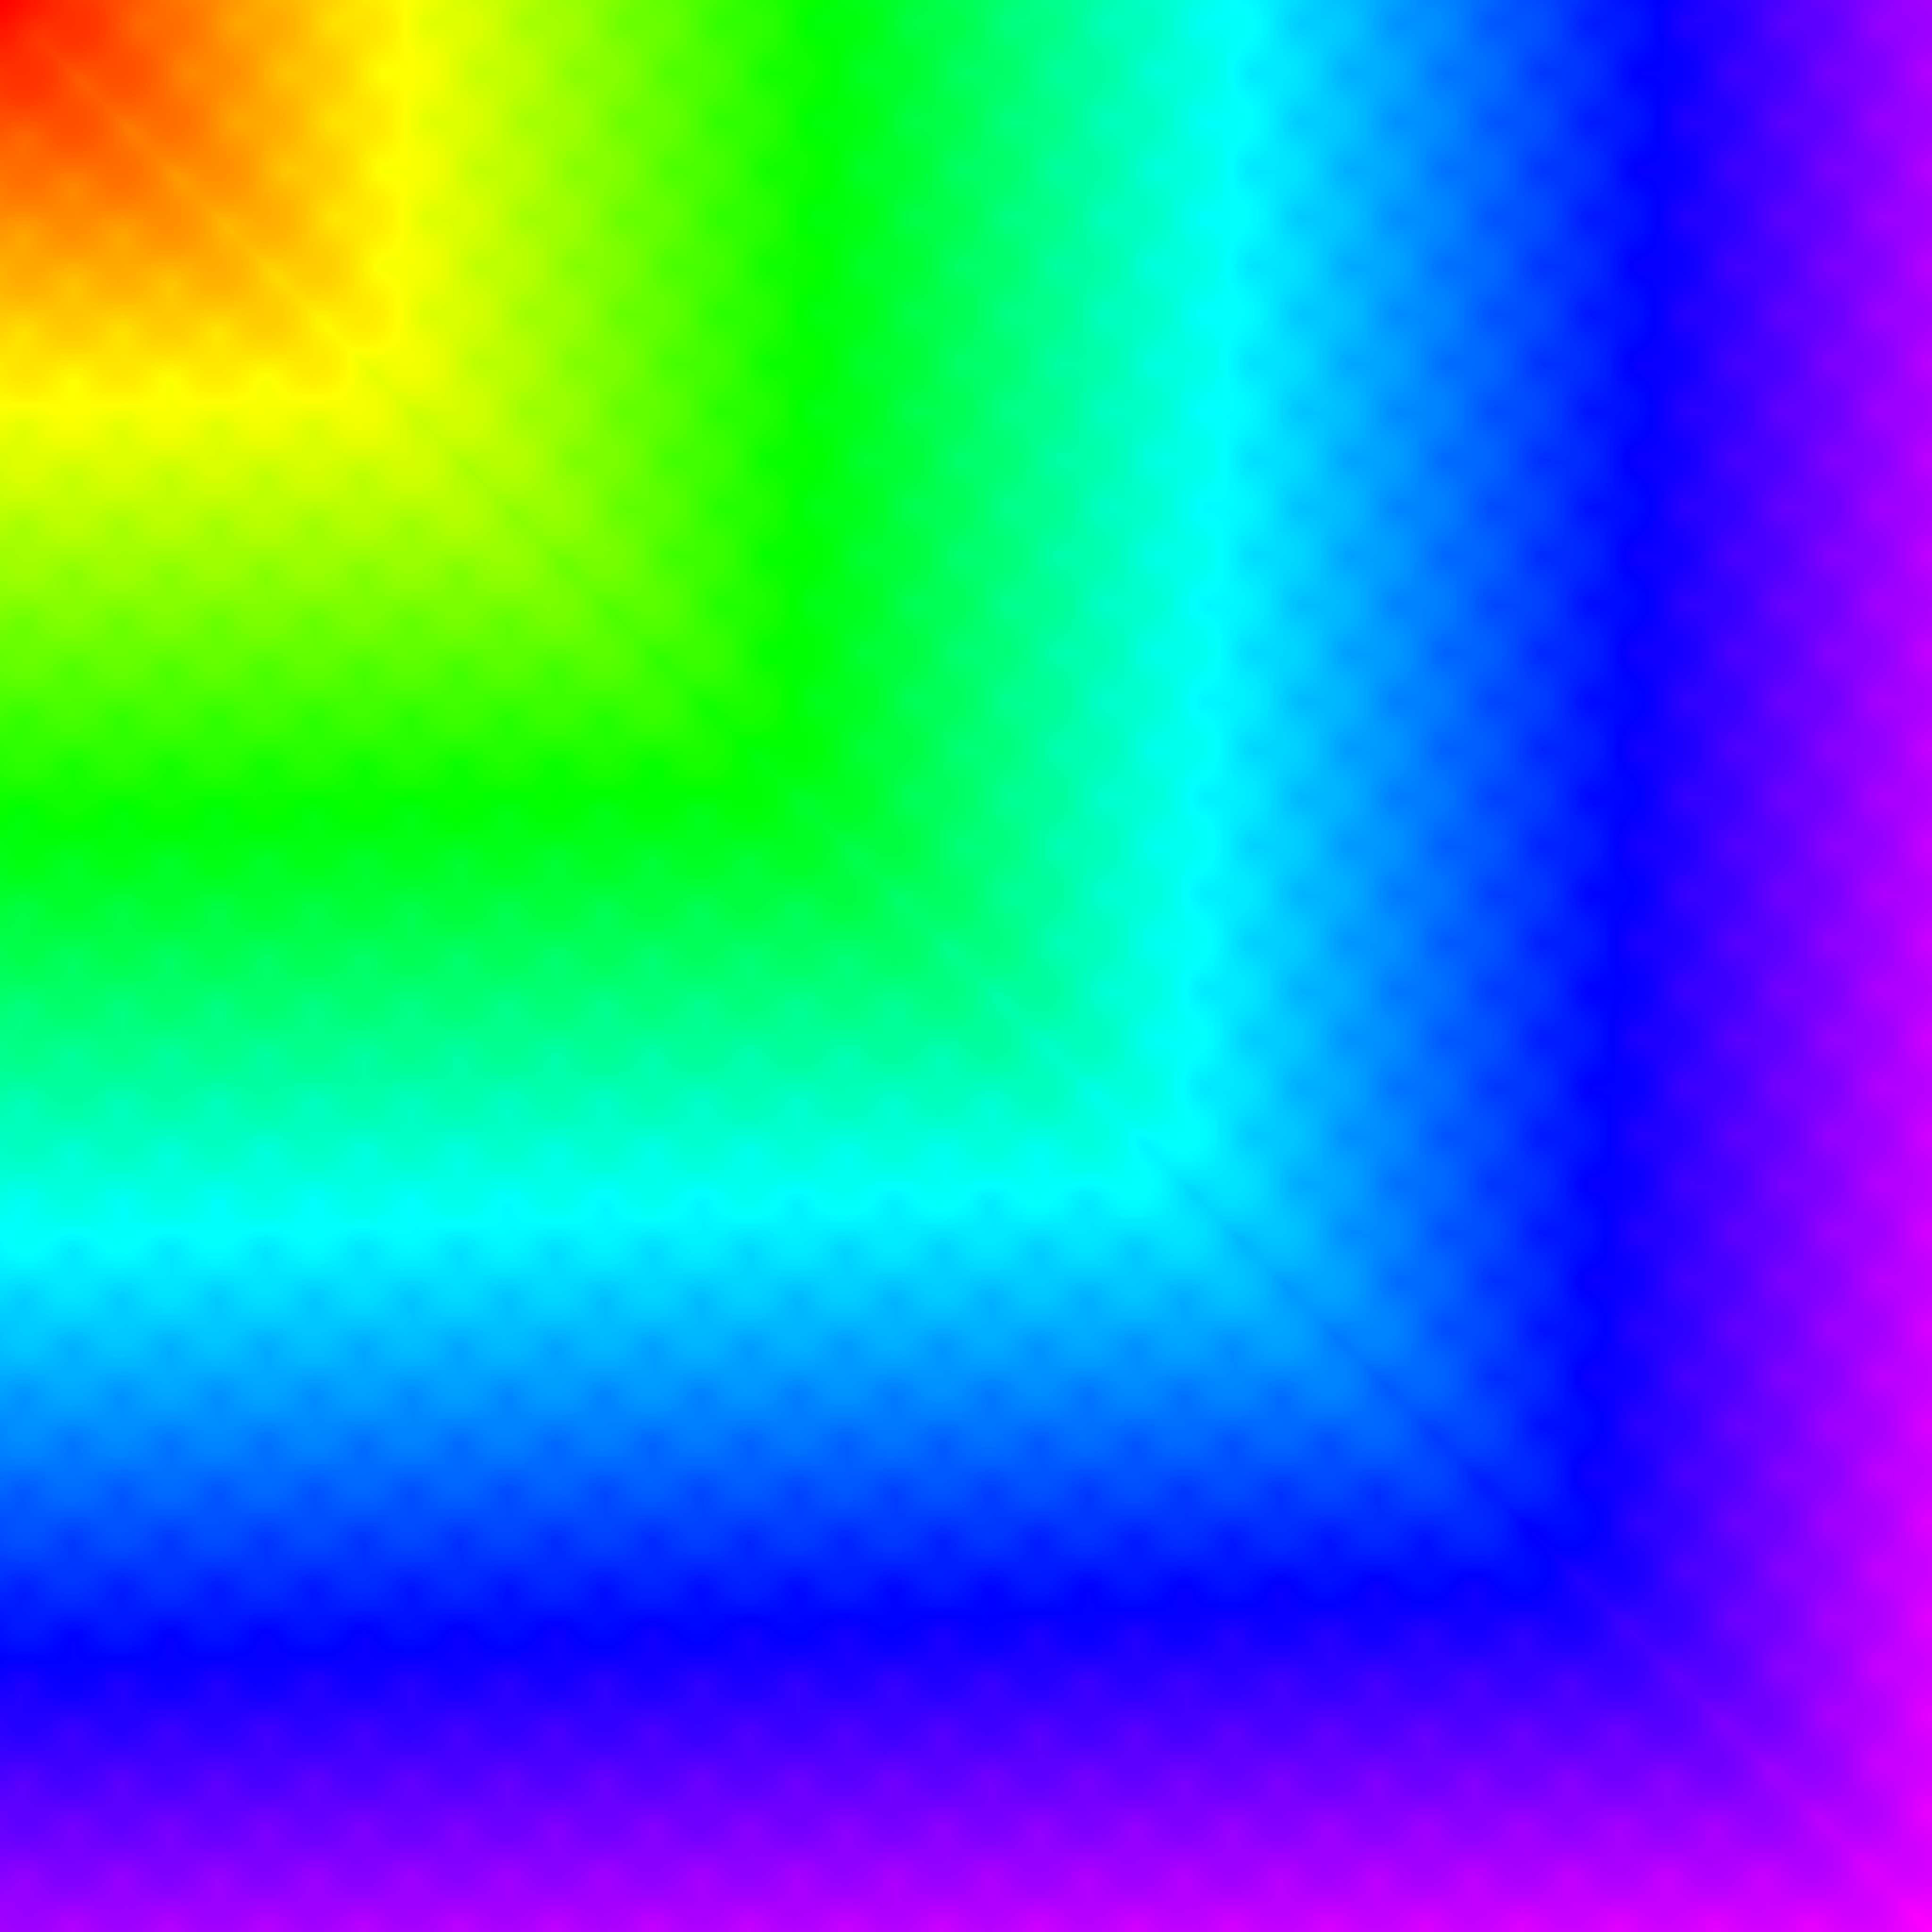
\includegraphics[width=\textwidth]{Figures/ghcm_systolic_sin_checkerboard}
	\end{subfigure}
	
	\begin{subfigure}[b]{.3\columnwidth}
		
\includegraphics[width=\textwidth]{Figures/fmm_7_rings}
		\caption{FMM}
	\end{subfigure}
	\begin{subfigure}[b]{.3\columnwidth}
		
\includegraphics[width=\textwidth]{Figures/fim_7_rings}
		\caption{FIM}
	\end{subfigure}
	\begin{subfigure}[b]{.3\columnwidth}
		
\includegraphics[width=\textwidth]{Figures/ghcm_systolic_7_rings}
		\caption{gHCM}
	\end{subfigure}
	
	\caption{Output of each algorithm for Constant, Sin Checkerboard, and 7-ring. (1 of 2)}
	\label{fig:output_1}
\end{figure}

\begin{figure}%[!b]
	\centering
	
	\begin{subfigure}[b]{.3\columnwidth}
		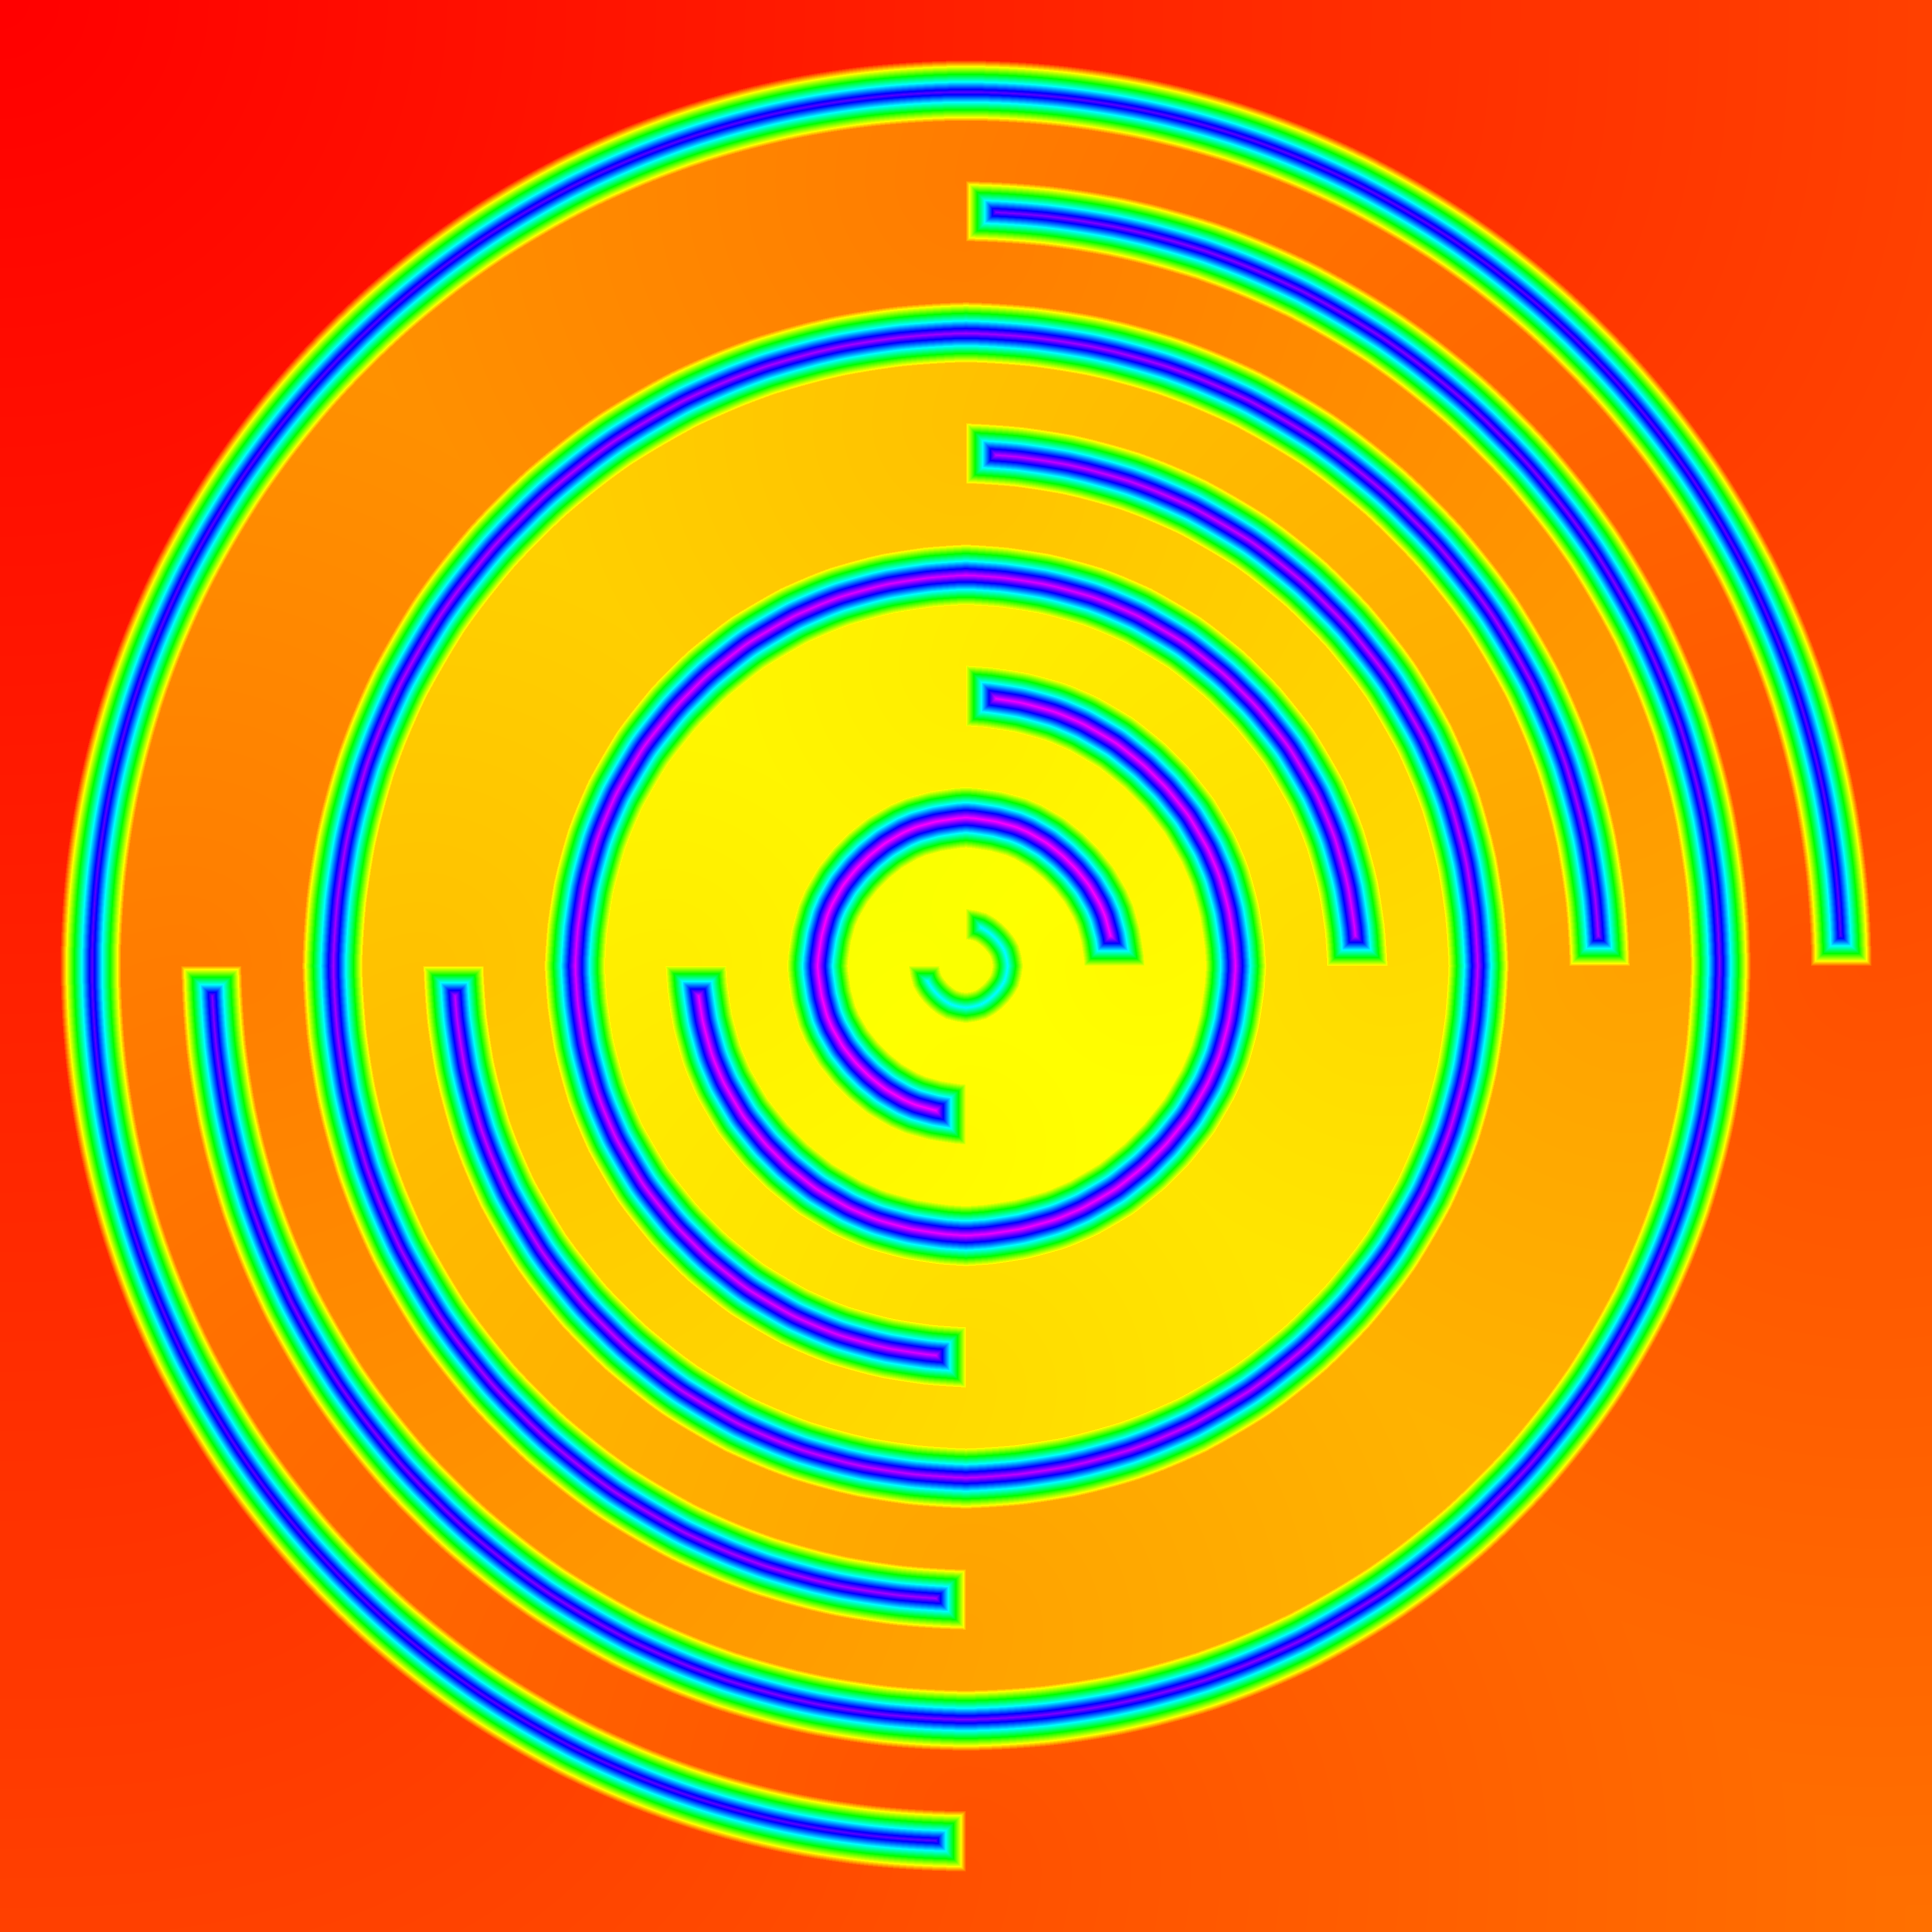
\includegraphics[width=\textwidth]{Figures/fmm_7_rings_permeable}
	\end{subfigure}
	\begin{subfigure}[b]{.3\columnwidth}
		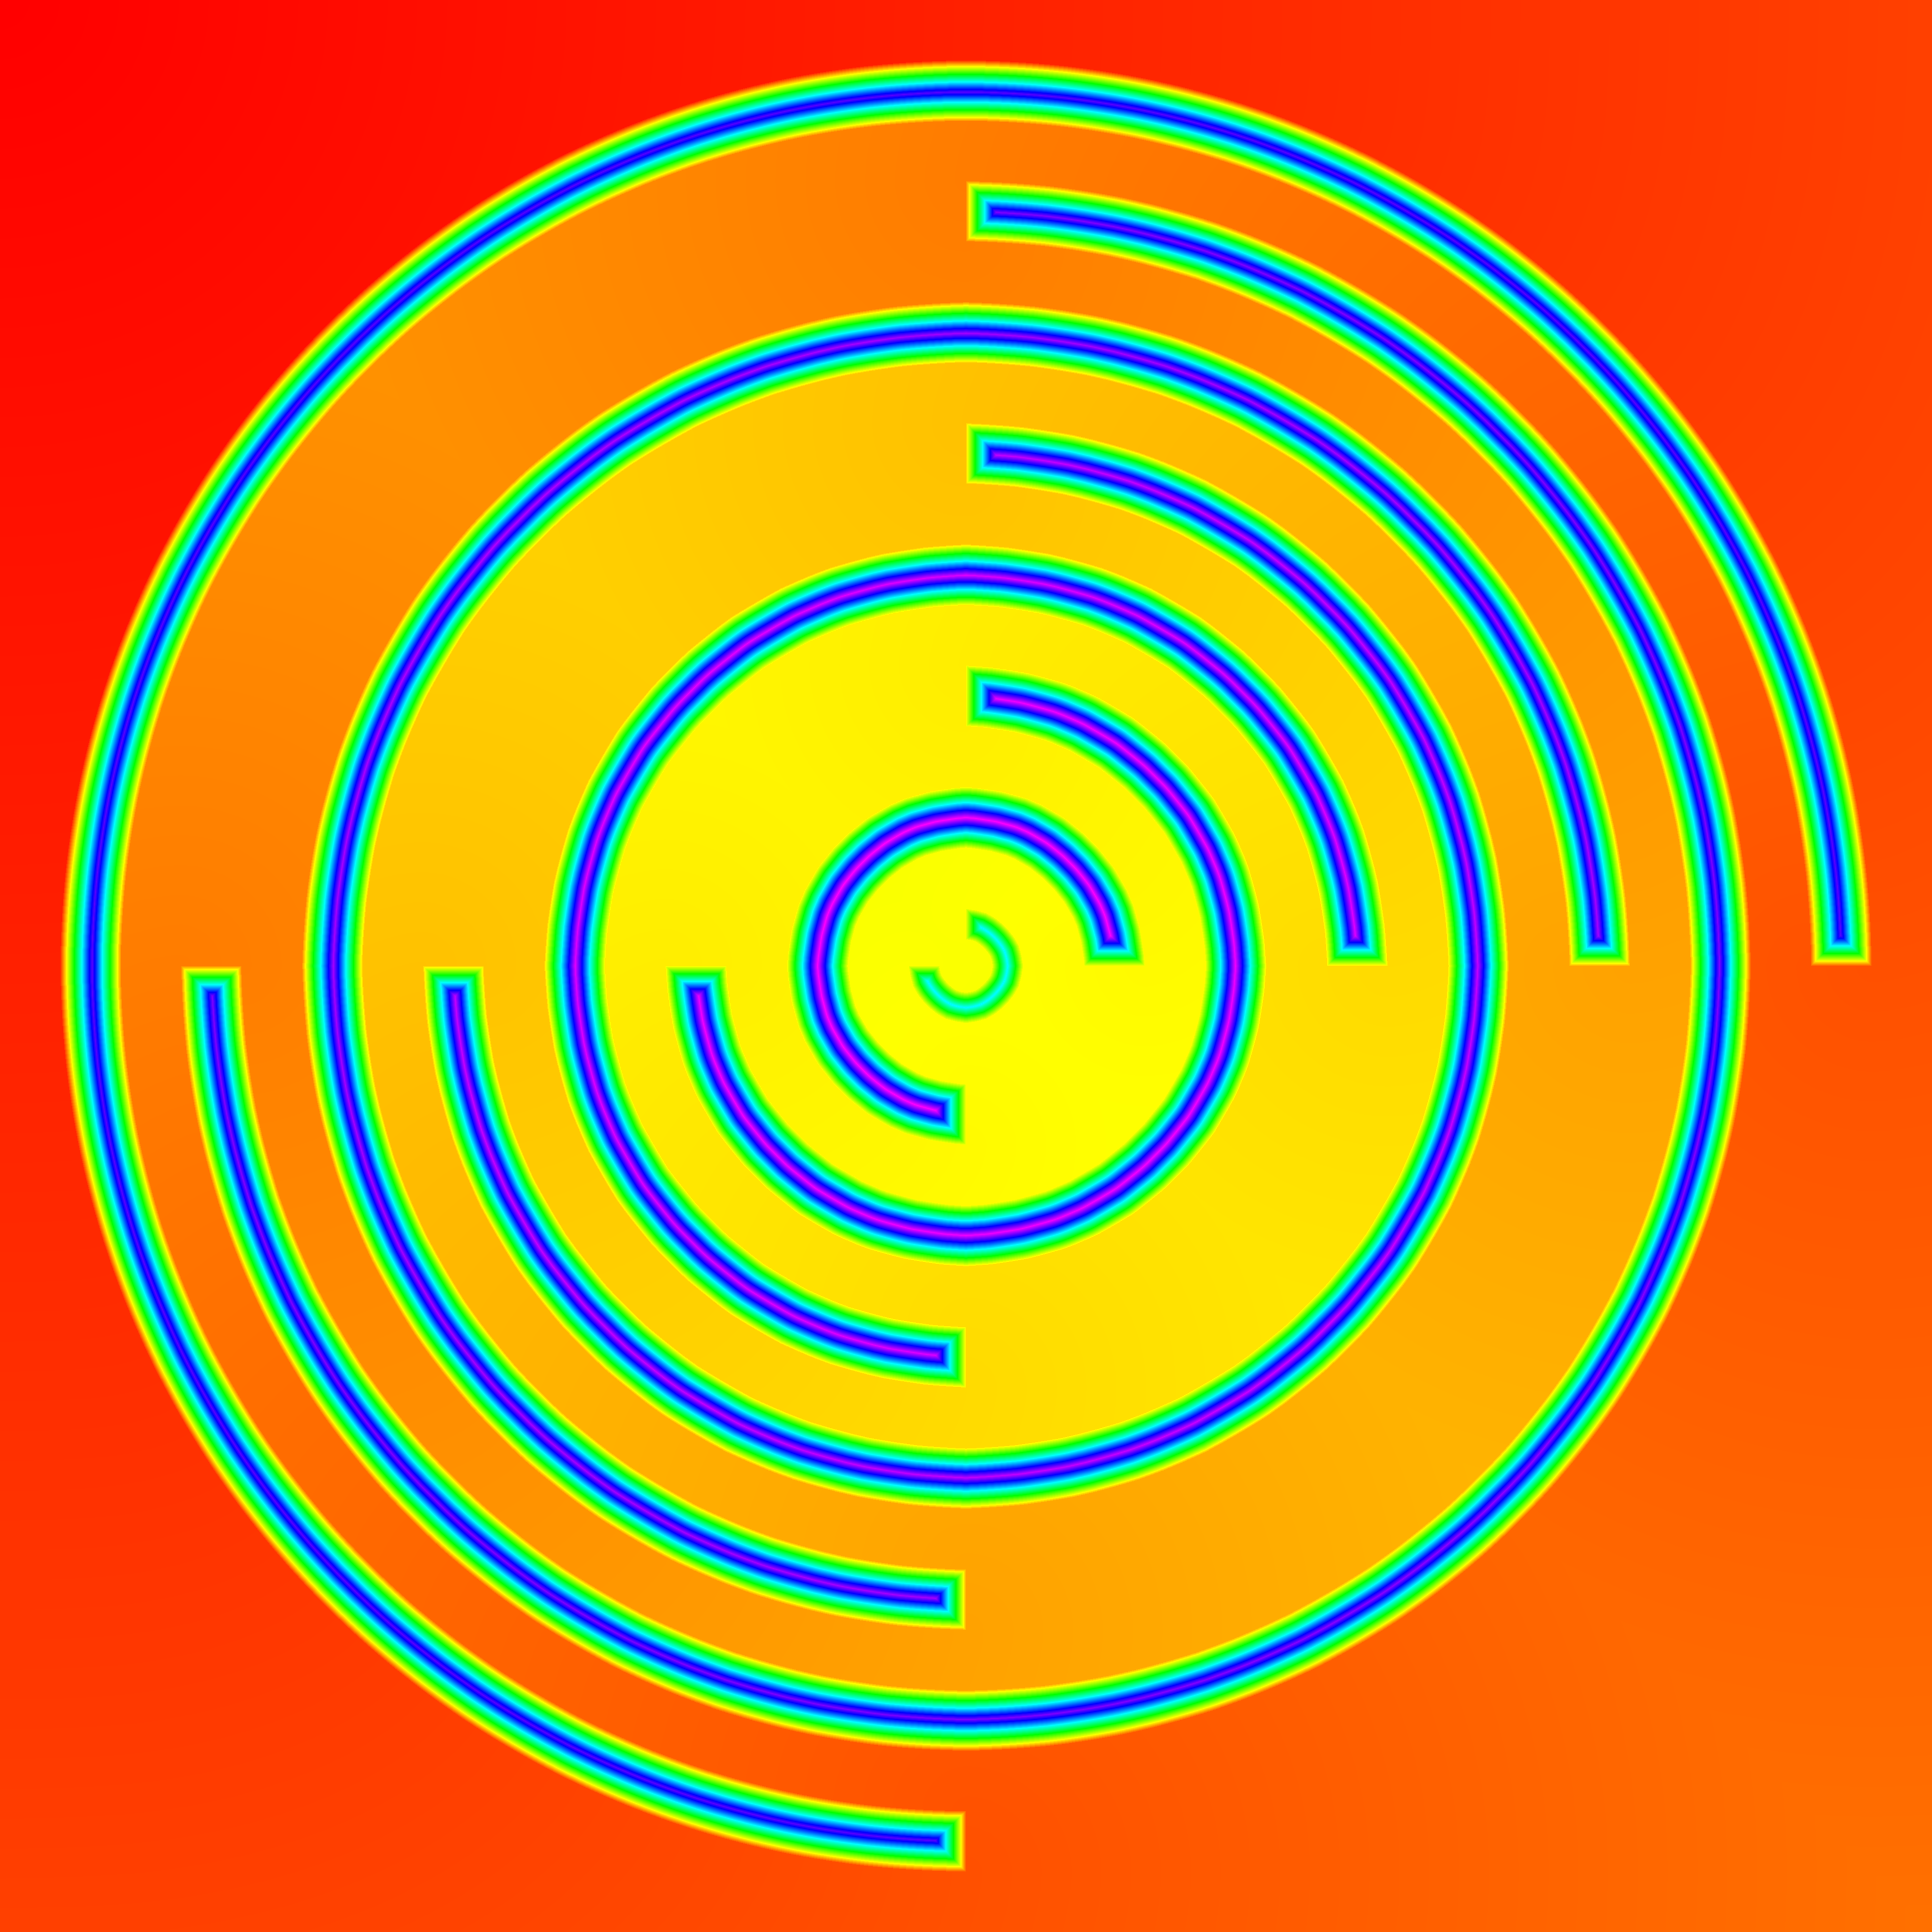
\includegraphics[width=\textwidth]{Figures/fim_7_rings_permeable}
	\end{subfigure}
	\begin{subfigure}[b]{.3\columnwidth}
		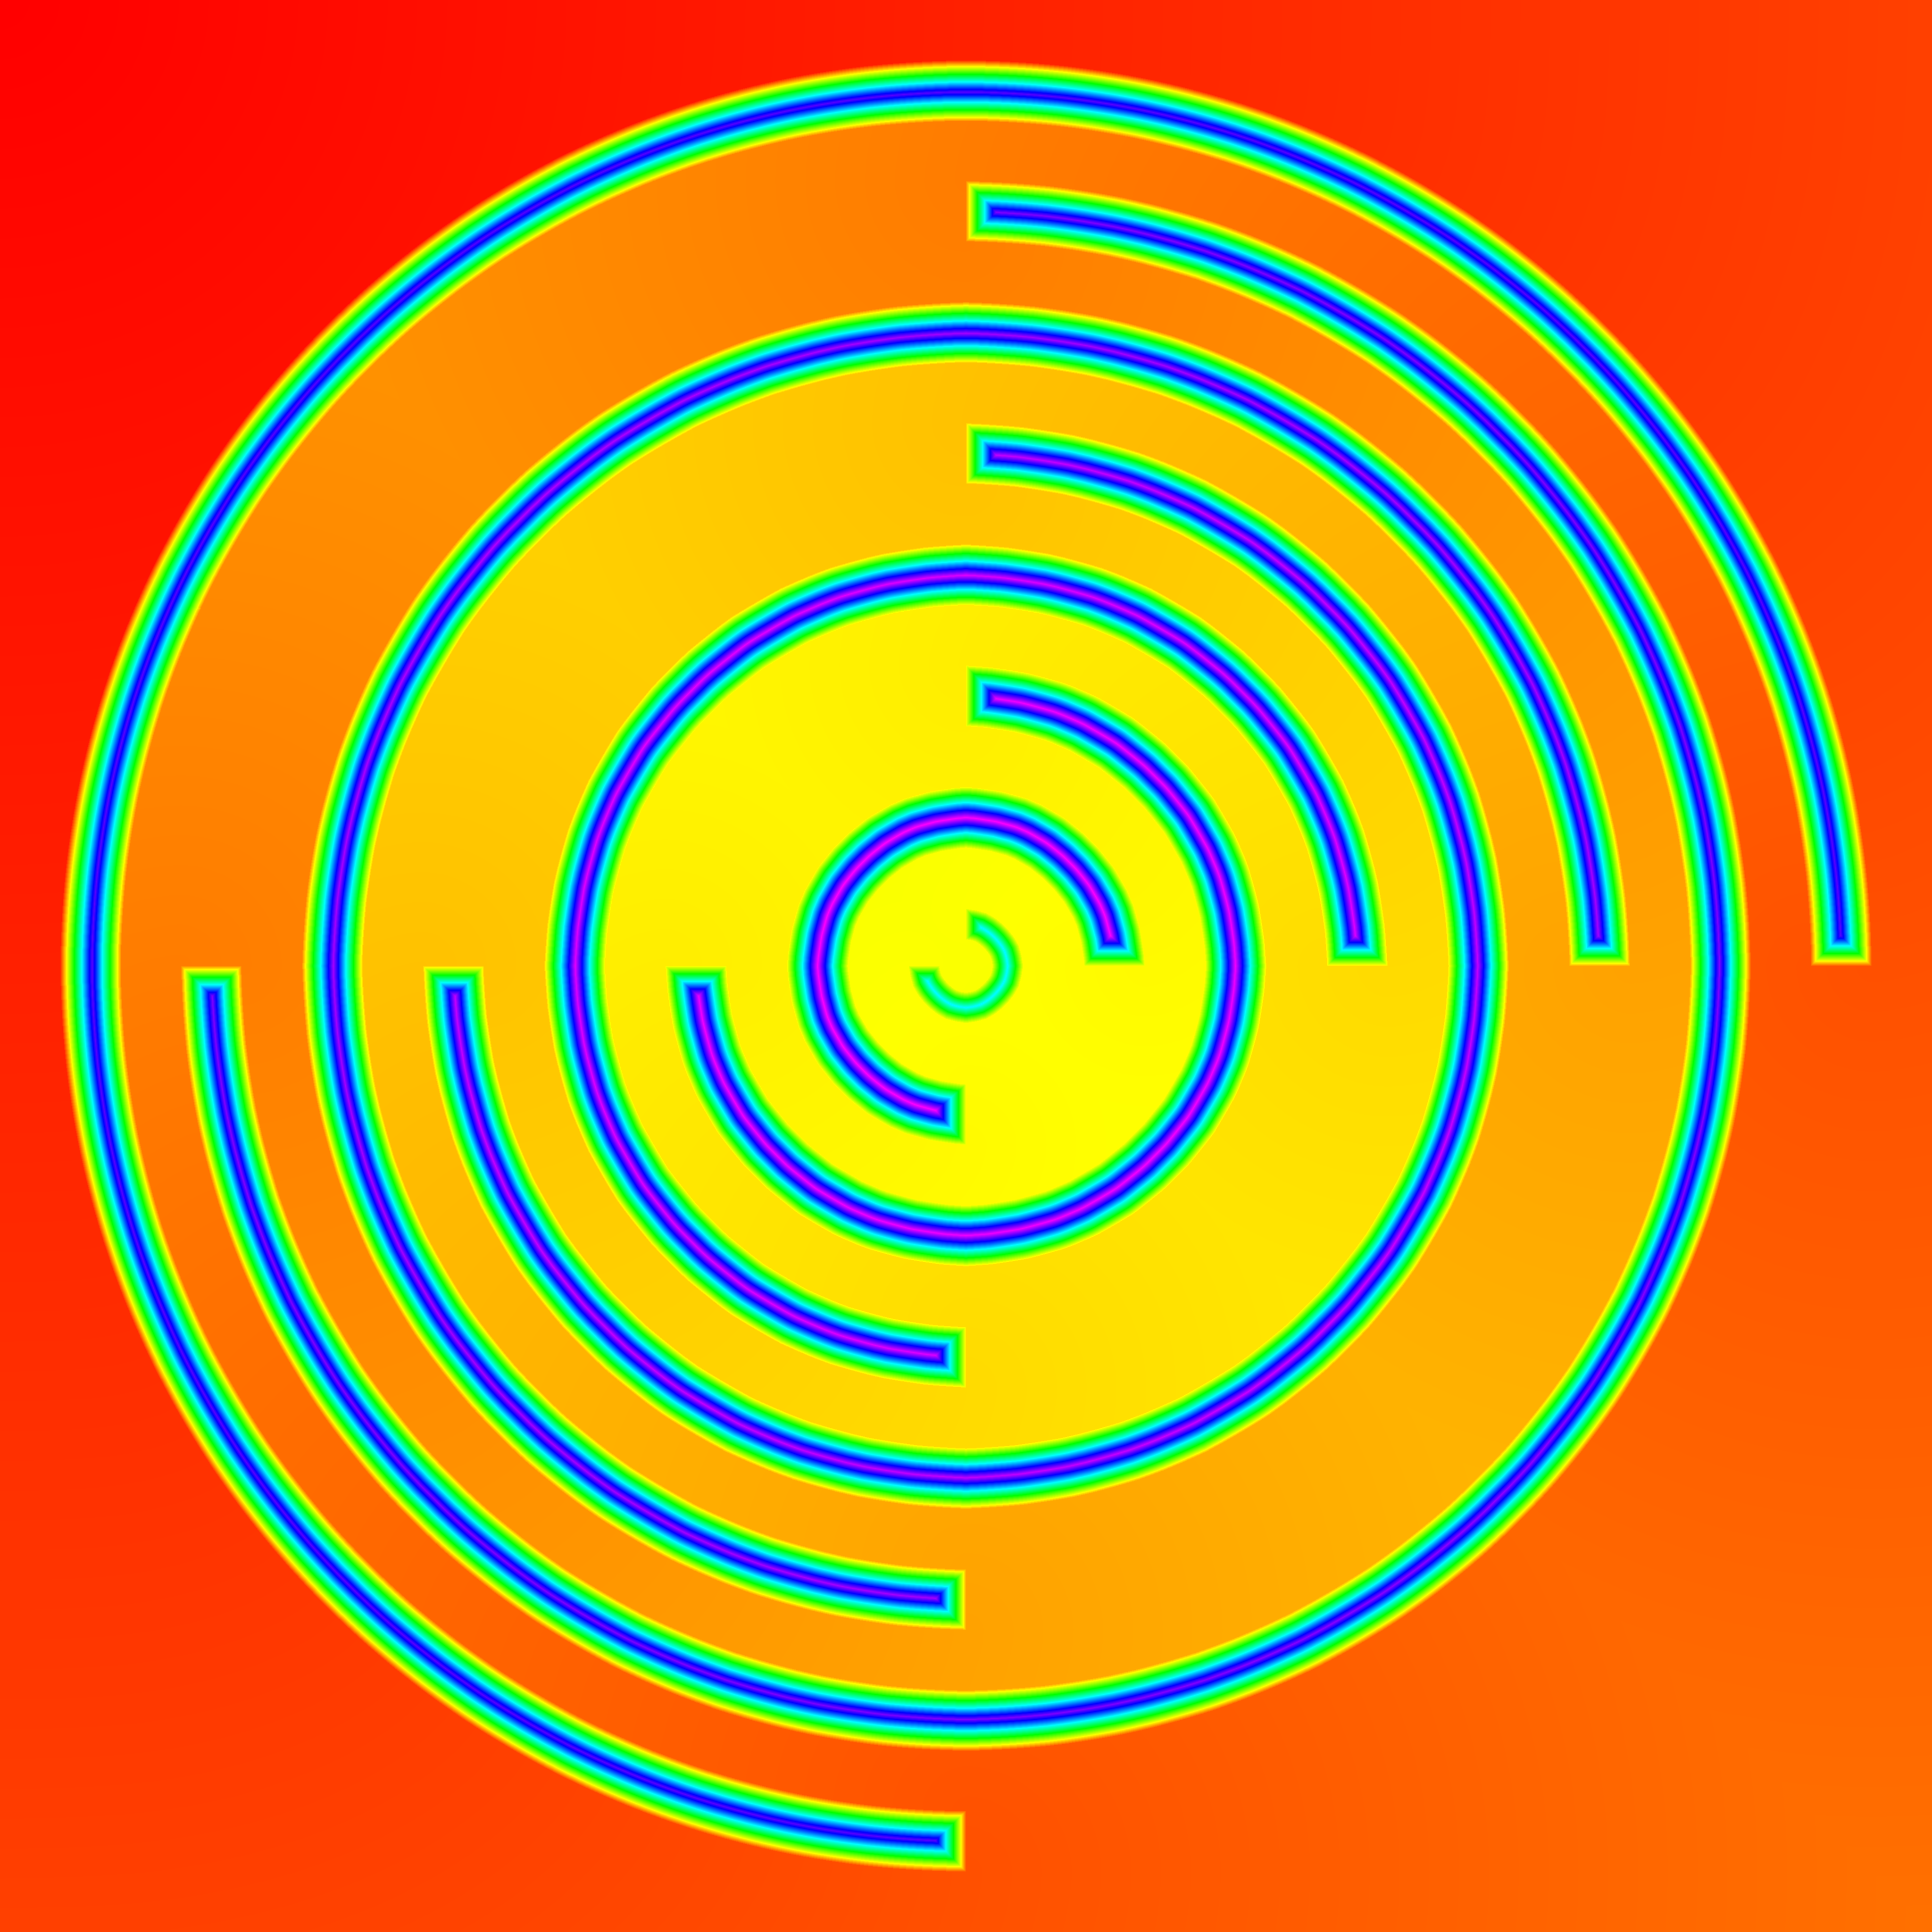
\includegraphics[width=\textwidth]{Figures/ghcm_systolic_7_rings_permeable}
	\end{subfigure}
	
	\begin{subfigure}[b]{.3\columnwidth}
		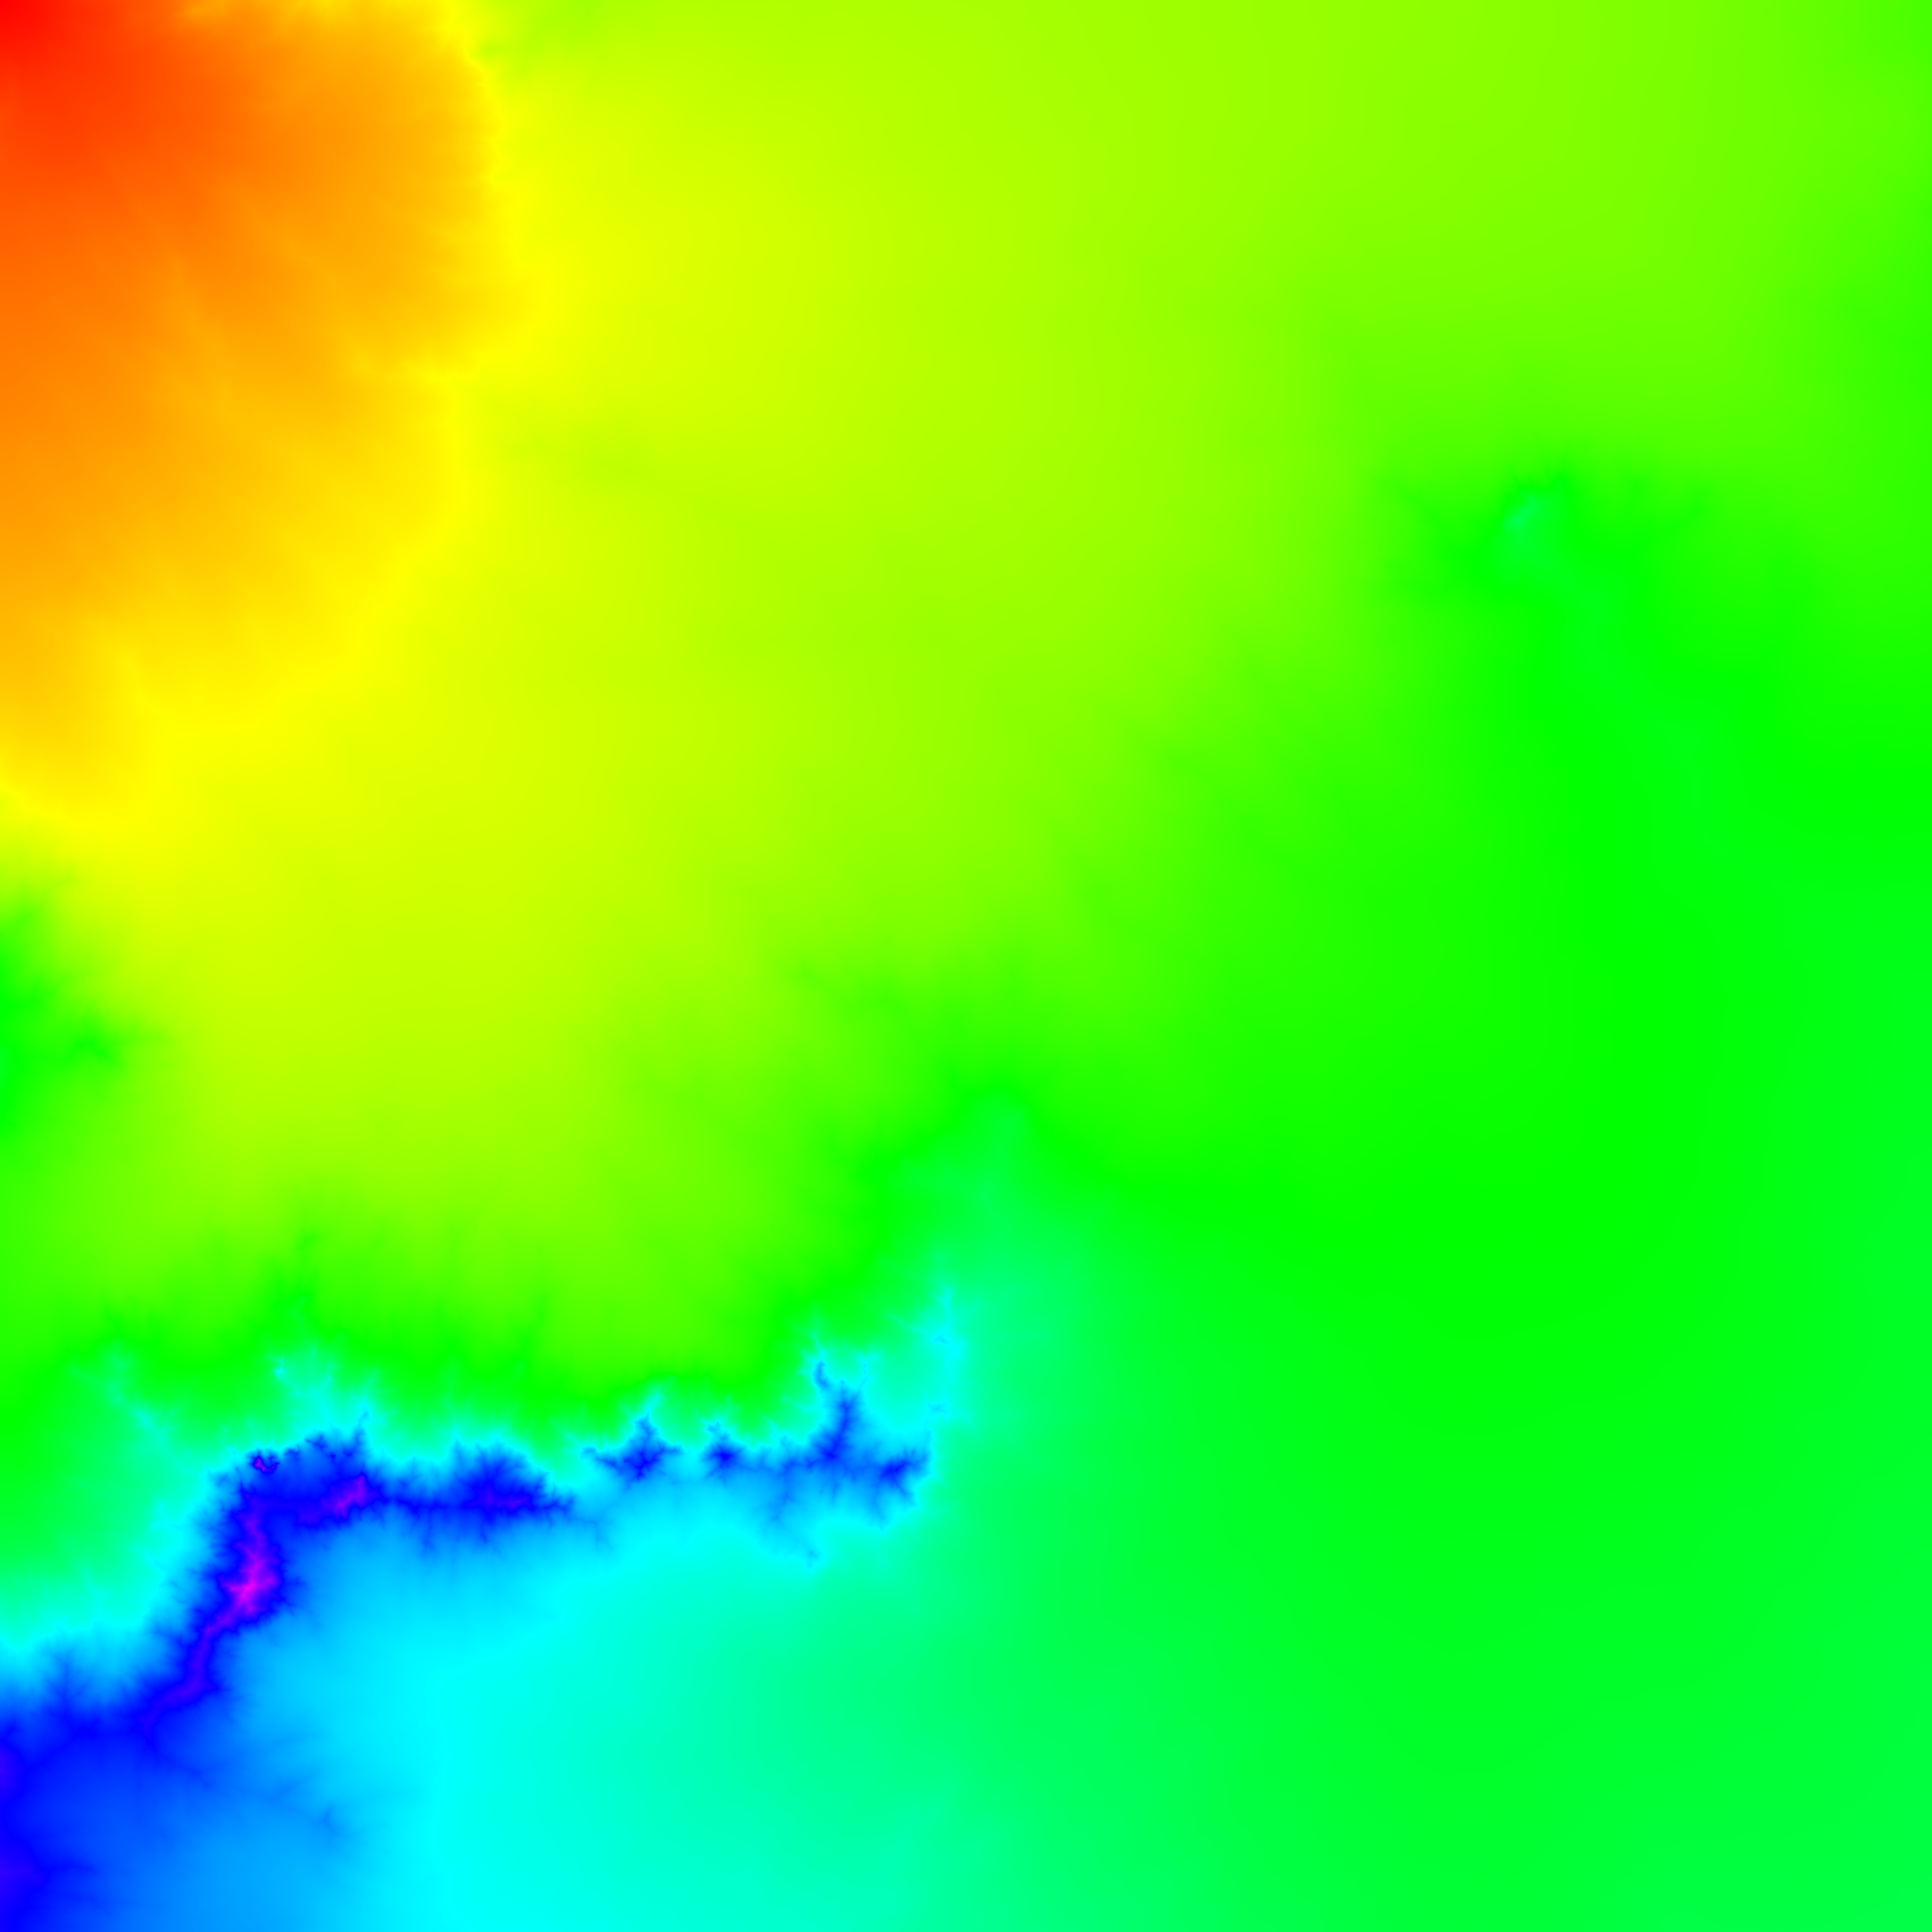
\includegraphics[width=\textwidth]{Figures/fmm_cloudy}
	\end{subfigure}
	\begin{subfigure}[b]{.3\columnwidth}
		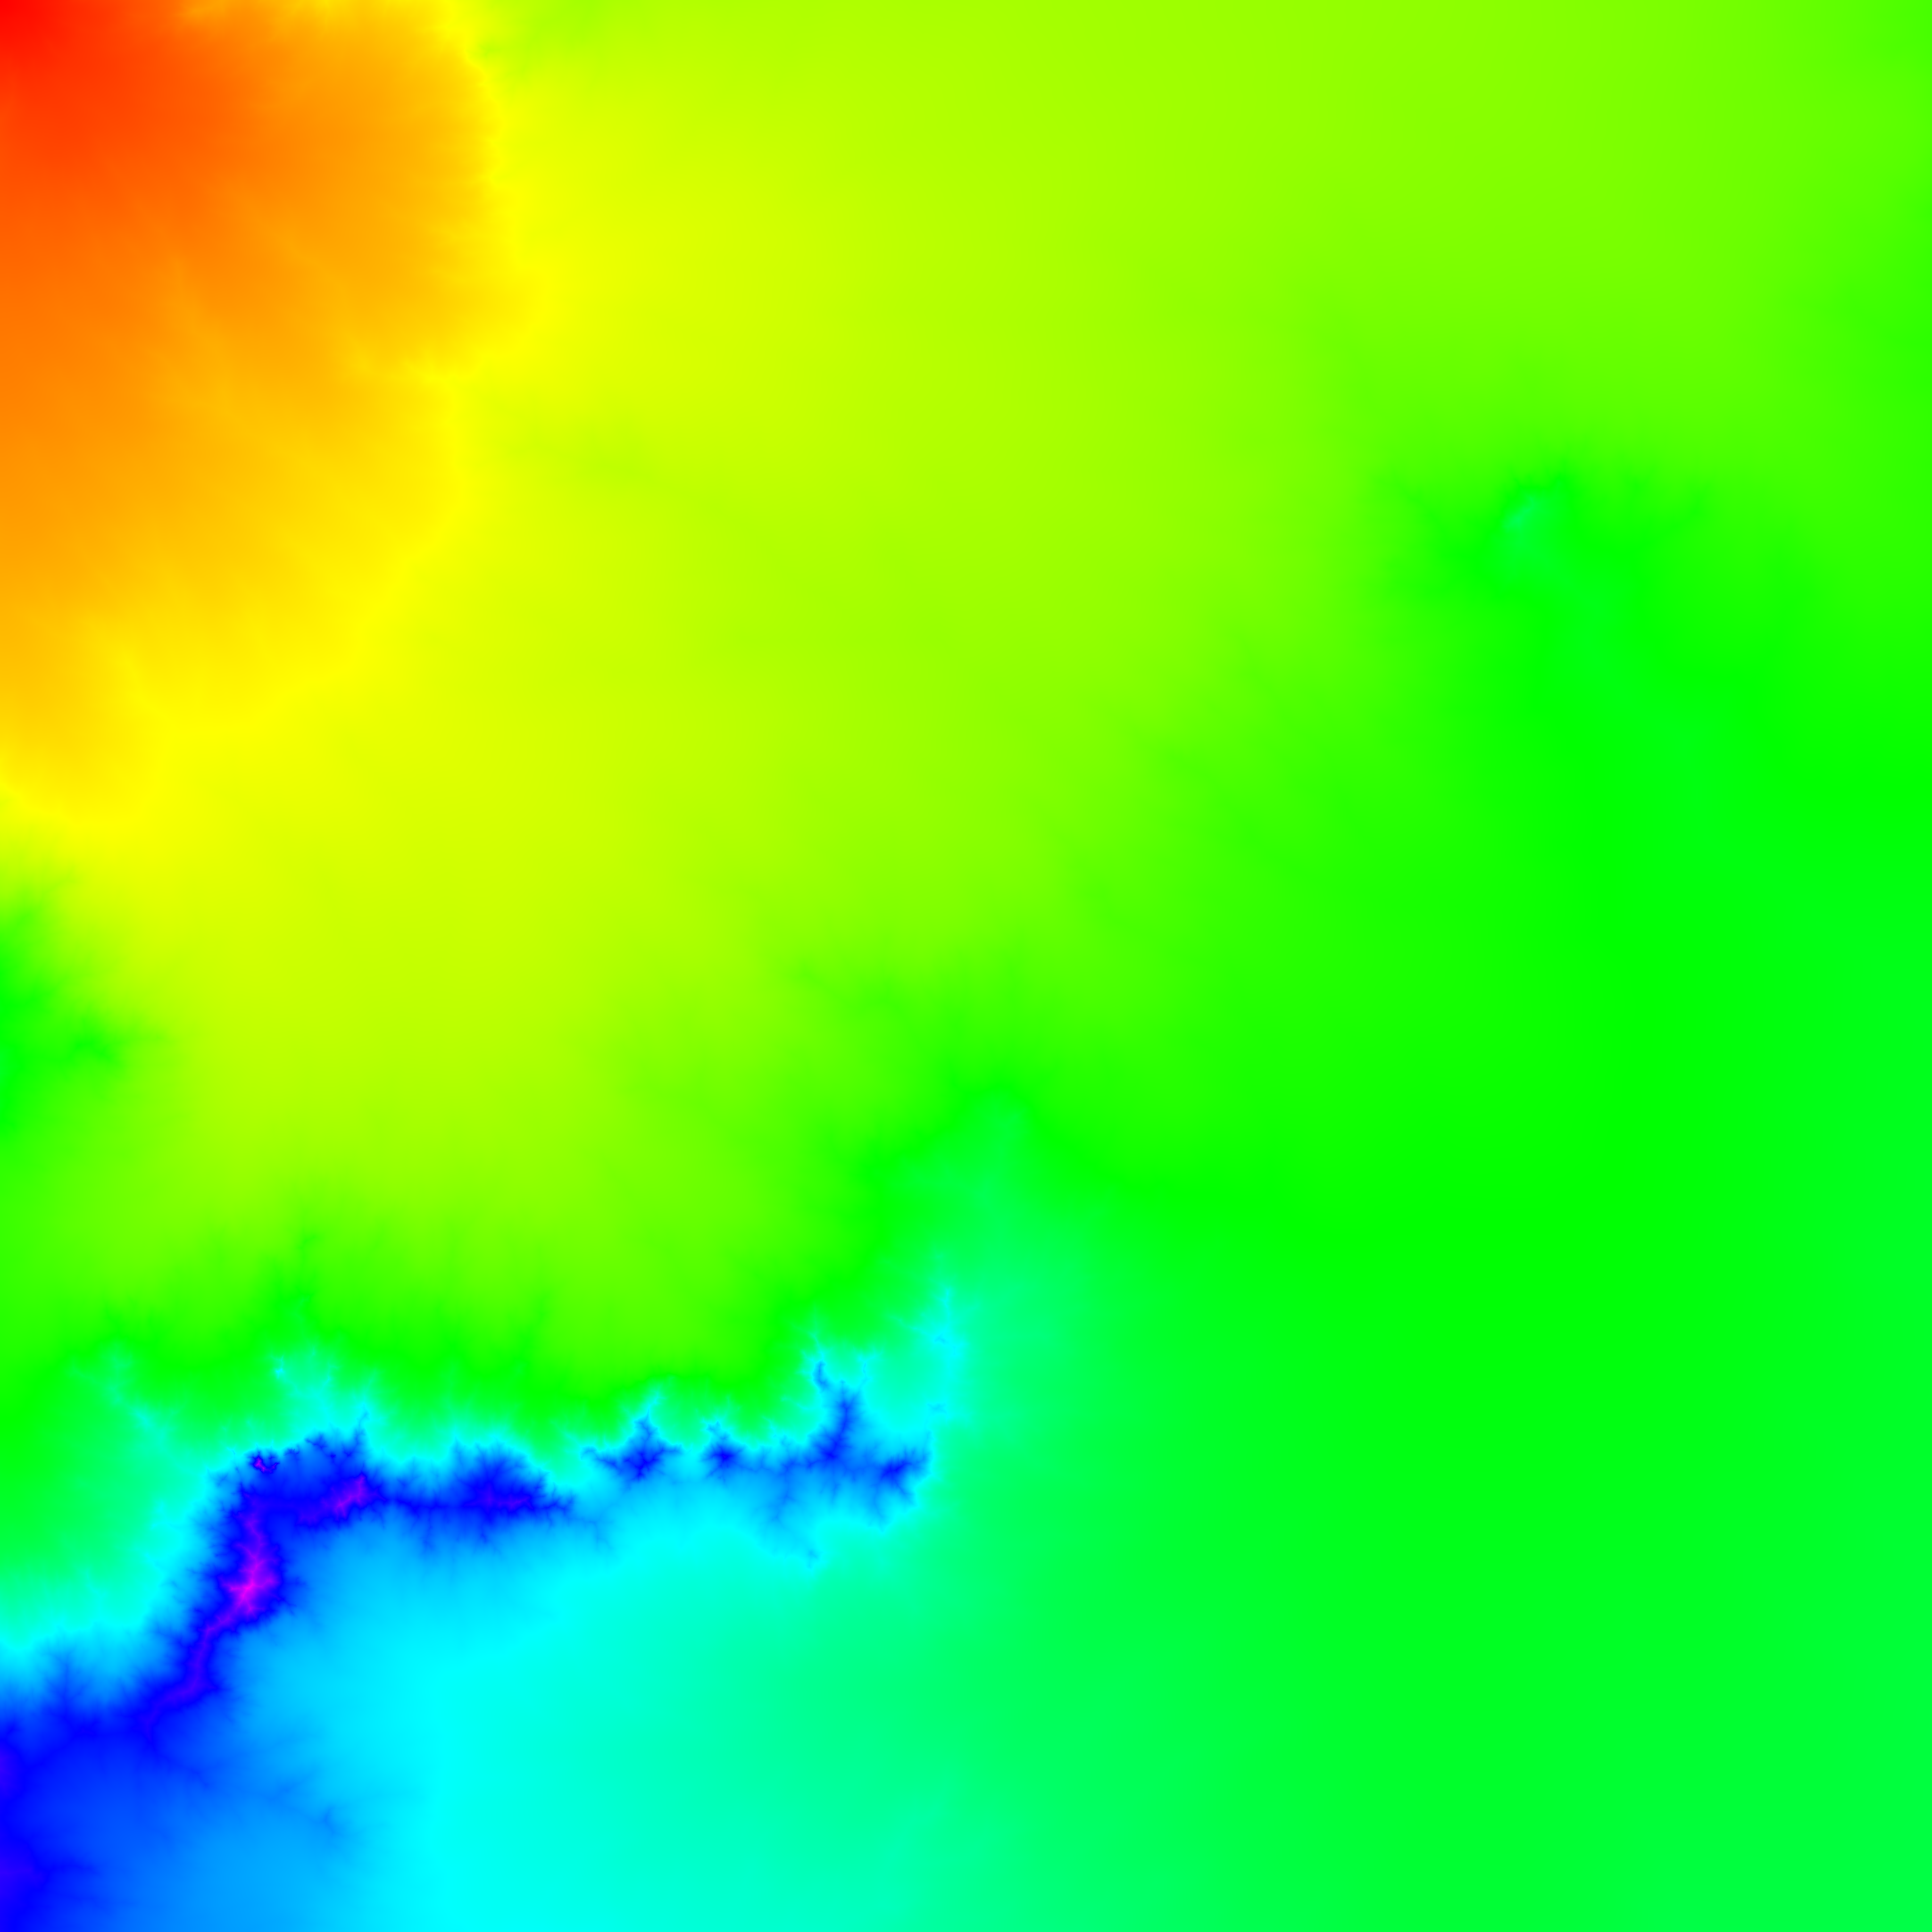
\includegraphics[width=\textwidth]{Figures/fim_cloudy}
	\end{subfigure}
	\begin{subfigure}[b]{.3\columnwidth}
		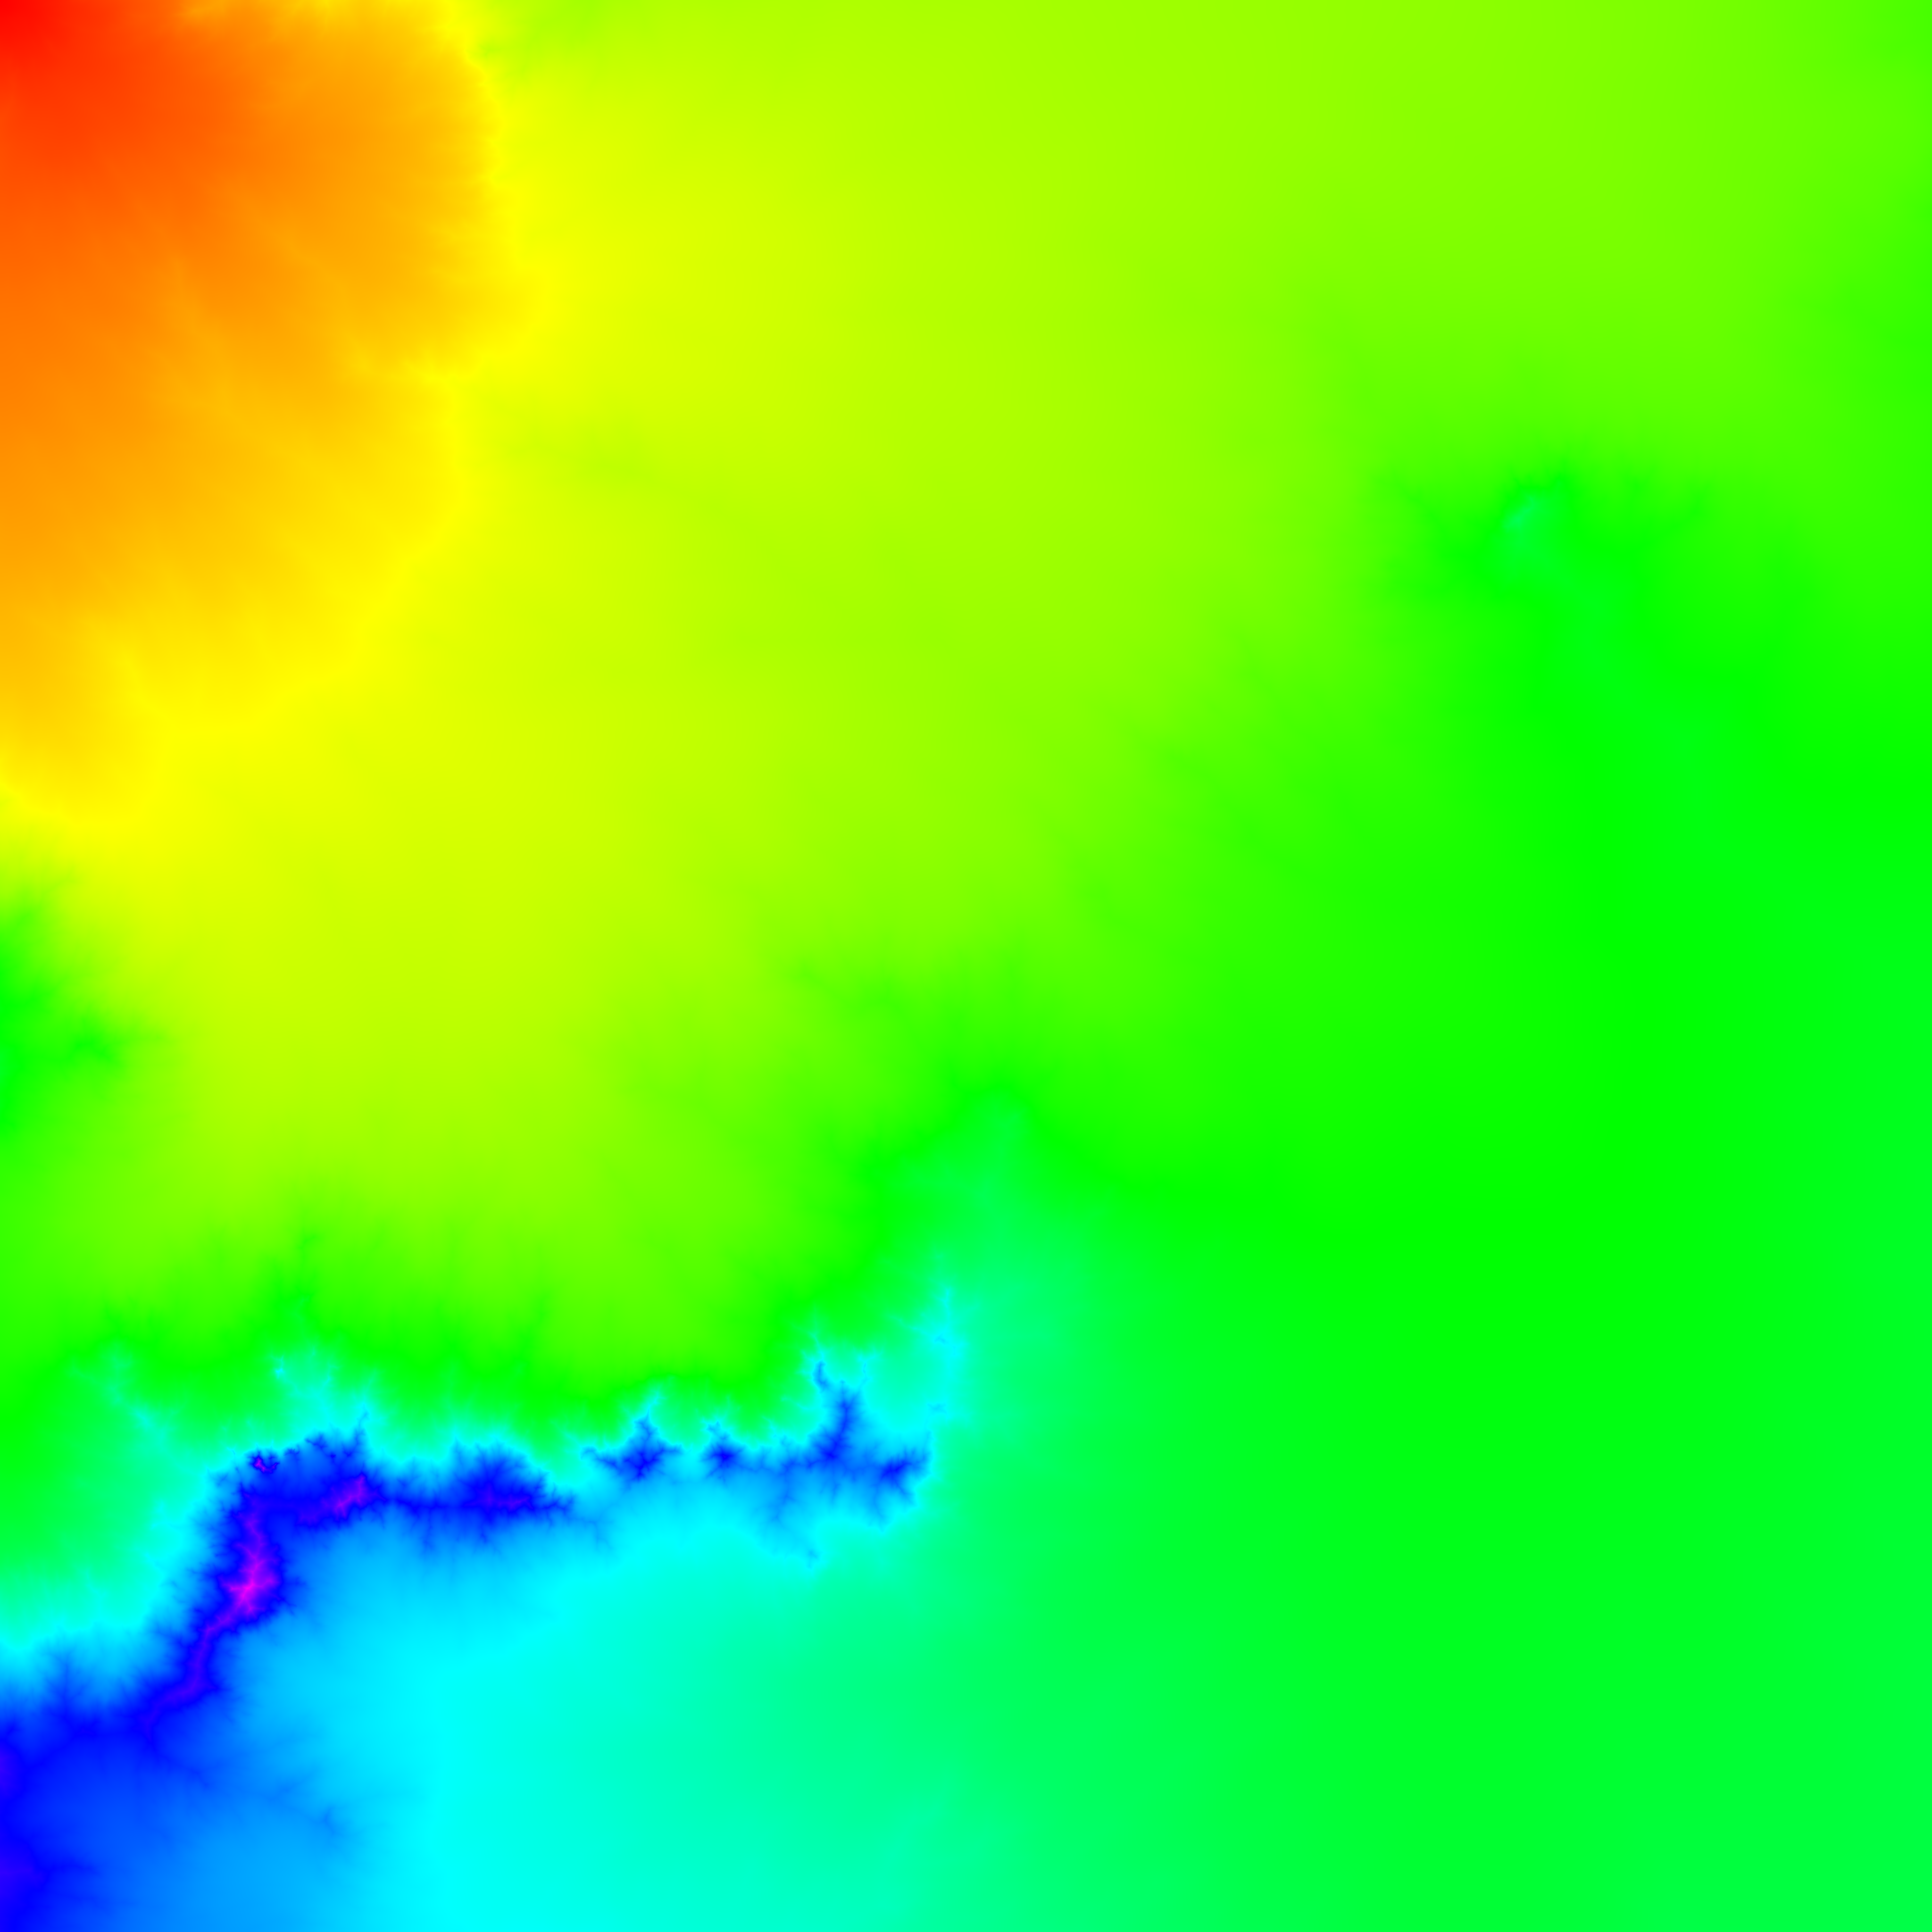
\includegraphics[width=\textwidth]{Figures/ghcm_systolic_cloudy}
	\end{subfigure}
	
	\begin{subfigure}[b]{.3\columnwidth}
		\includegraphics[width=\textwidth]{Figures/fmm_photograph}
		\caption{FMM}
	\end{subfigure}
	\begin{subfigure}[b]{.3\columnwidth}
		\includegraphics[width=\textwidth]{Figures/fim_photograph}
		\caption{FIM}
	\end{subfigure}
	\begin{subfigure}[b]{.3\columnwidth}
		\includegraphics[width=\textwidth]{Figures/ghcm_systolic_photograph}
		\caption{gHCM}
	\end{subfigure}
	
	\caption{Output of each algorithm for 7-ring permeable, Cloudy, and Photograph. (2 of 2)}
	\label{fig:output_2}
\end{figure}

\begin{figure}%[!b]
	\centering
	\begin{subfigure}[b]{.4\columnwidth}
		\includegraphics[width=\textwidth]{Figures/diff_constant}
		\caption{Constant: $[-.1665, .0141]$}
	\end{subfigure}
	\begin{subfigure}[b]{.4\columnwidth}
		
\includegraphics[width=\textwidth]{Figures/diff_sin_checkerboard}
		\caption{Sin Checkerboard: $[-.0178, 2.217]$}
	\end{subfigure}
	\begin{subfigure}[b]{.4\columnwidth}
		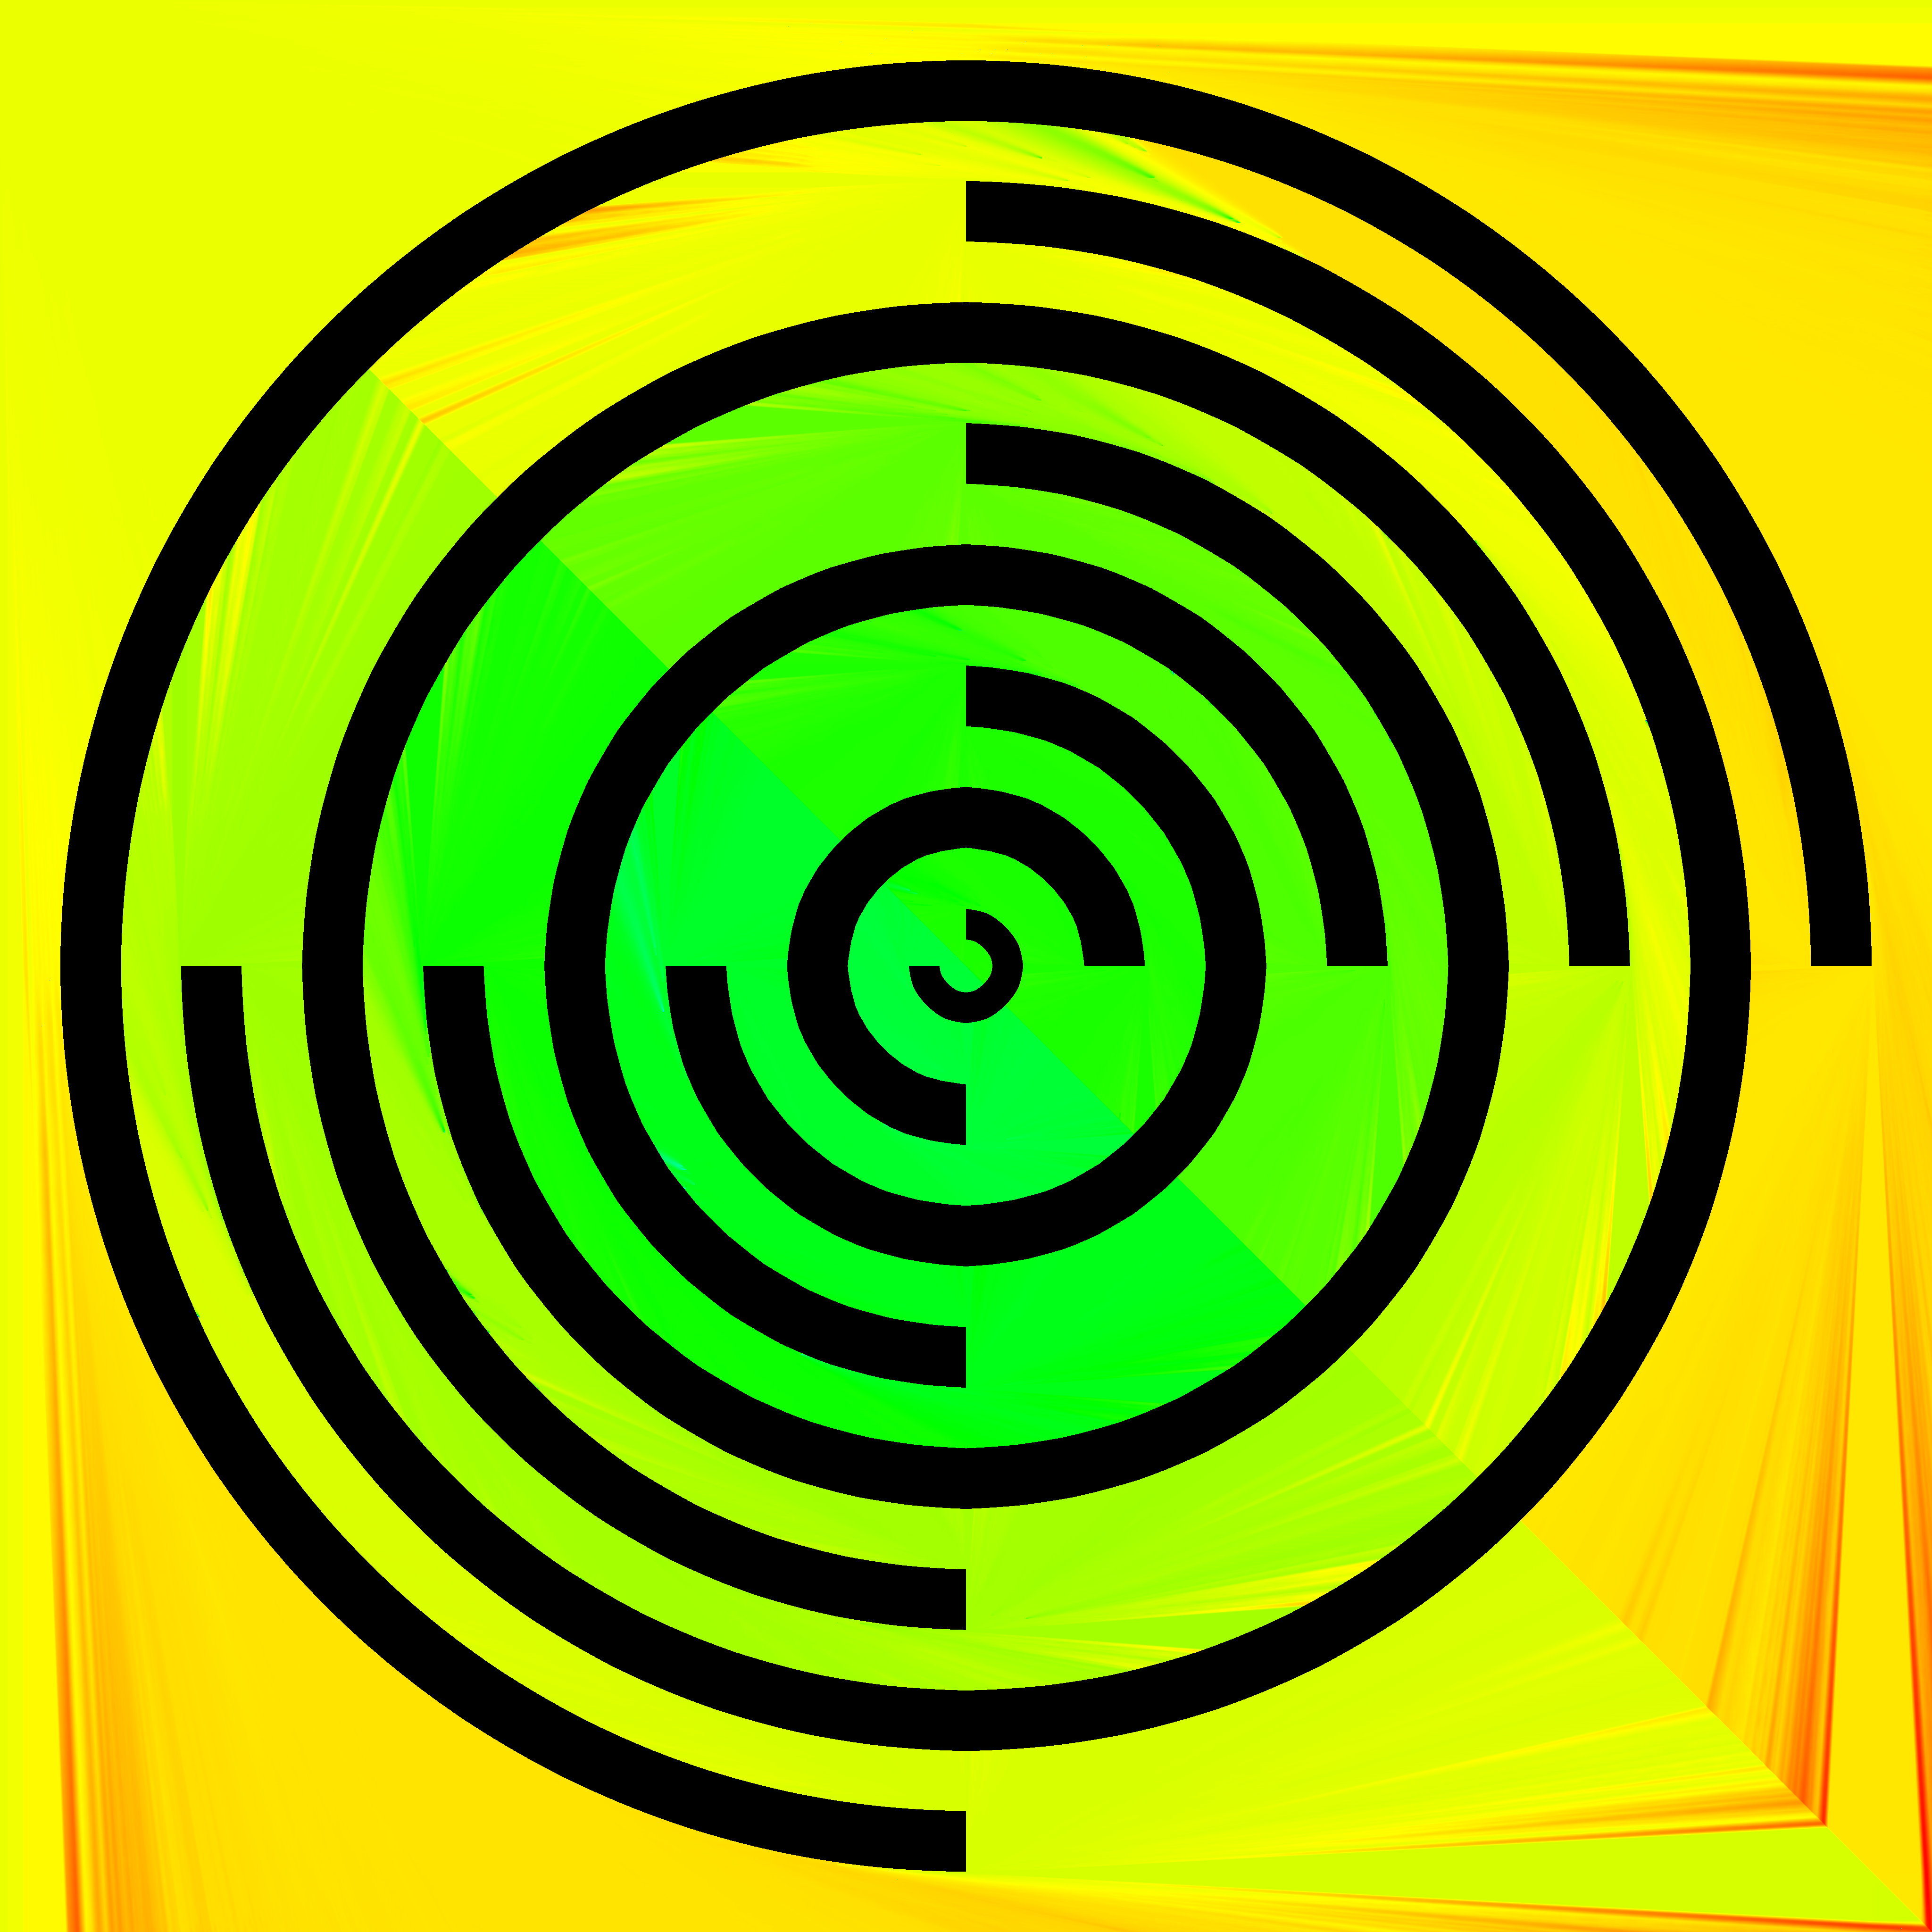
\includegraphics[width=\textwidth]{Figures/diff_7_rings}
		\caption{7-Ring: $[-.2768, 1.012]$}
	\end{subfigure}
	\begin{subfigure}[b]{.4\columnwidth}
		
\includegraphics[width=\textwidth]{Figures/diff_7_rings_permeable}
		\caption{7-Ring Permeable: $[-.5551, 1465]$}
	\end{subfigure}
	\begin{subfigure}[b]{.4\columnwidth}
		
\includegraphics[width=\textwidth]{Figures/diff_cloudy}
		\caption{Cloudy: $[-.3437, 79.57]$}
	\end{subfigure}
	\begin{subfigure}[b]{.4\columnwidth}
		
\includegraphics[width=\textwidth]{Figures/diff_photograph}
		\caption{Photograph: $[-.0009155, 1.501]$}
	\end{subfigure}
	\caption{Relative error of gHCM-systolic to FMM (i.e. $output_{ghcm} - output_{fmm}$). Hue'd from Red (lower bound) to Magenta (upper bound). In certain cases a high error bound might be a point failure. See \autoref{sec:conclusion}.}
	\label{fig:rel_error_output}
\end{figure}



\subsection{Performance}

There are a number of configurable parameters that depend on the hardware in question. (See \autoref{sec:design}.) \autoref{fig:perf_results_main_1} and \autoref{fig:perf_results_main_2} contains the runtime for each test case against sequential FMM, sequential FIM, and a number of gHCM configurations.

We do not present a traditional speed-up graph. This is due to the fact that our method is not strictly about enabling as much parallelism as possible, but making better use of available hardware. That said, given the structure of our approach we can claim that the maximum speed-up is essentially FIM's (set $k=\infty$, and forgo ordering the open set when $k = \infty$). A rough estimate of how a Block FIM implementation might perform can be gained by looking at entries for gHCM-systolic with a high compute-overload (CU) in the performance plot. Note that even in the high compute-overload cases listed (e.g. 32), the open-set frequently remains greater than the bundles dispatched. (e.g. Compute-overload 32 with 32 compute units yields a bundle of 1024, yet the open-set can reach four thousand in 7-ring permeable.)

\begin{figure}%[!b]
	\centering
	\begin{subfigure}[b]{.4\columnwidth}
		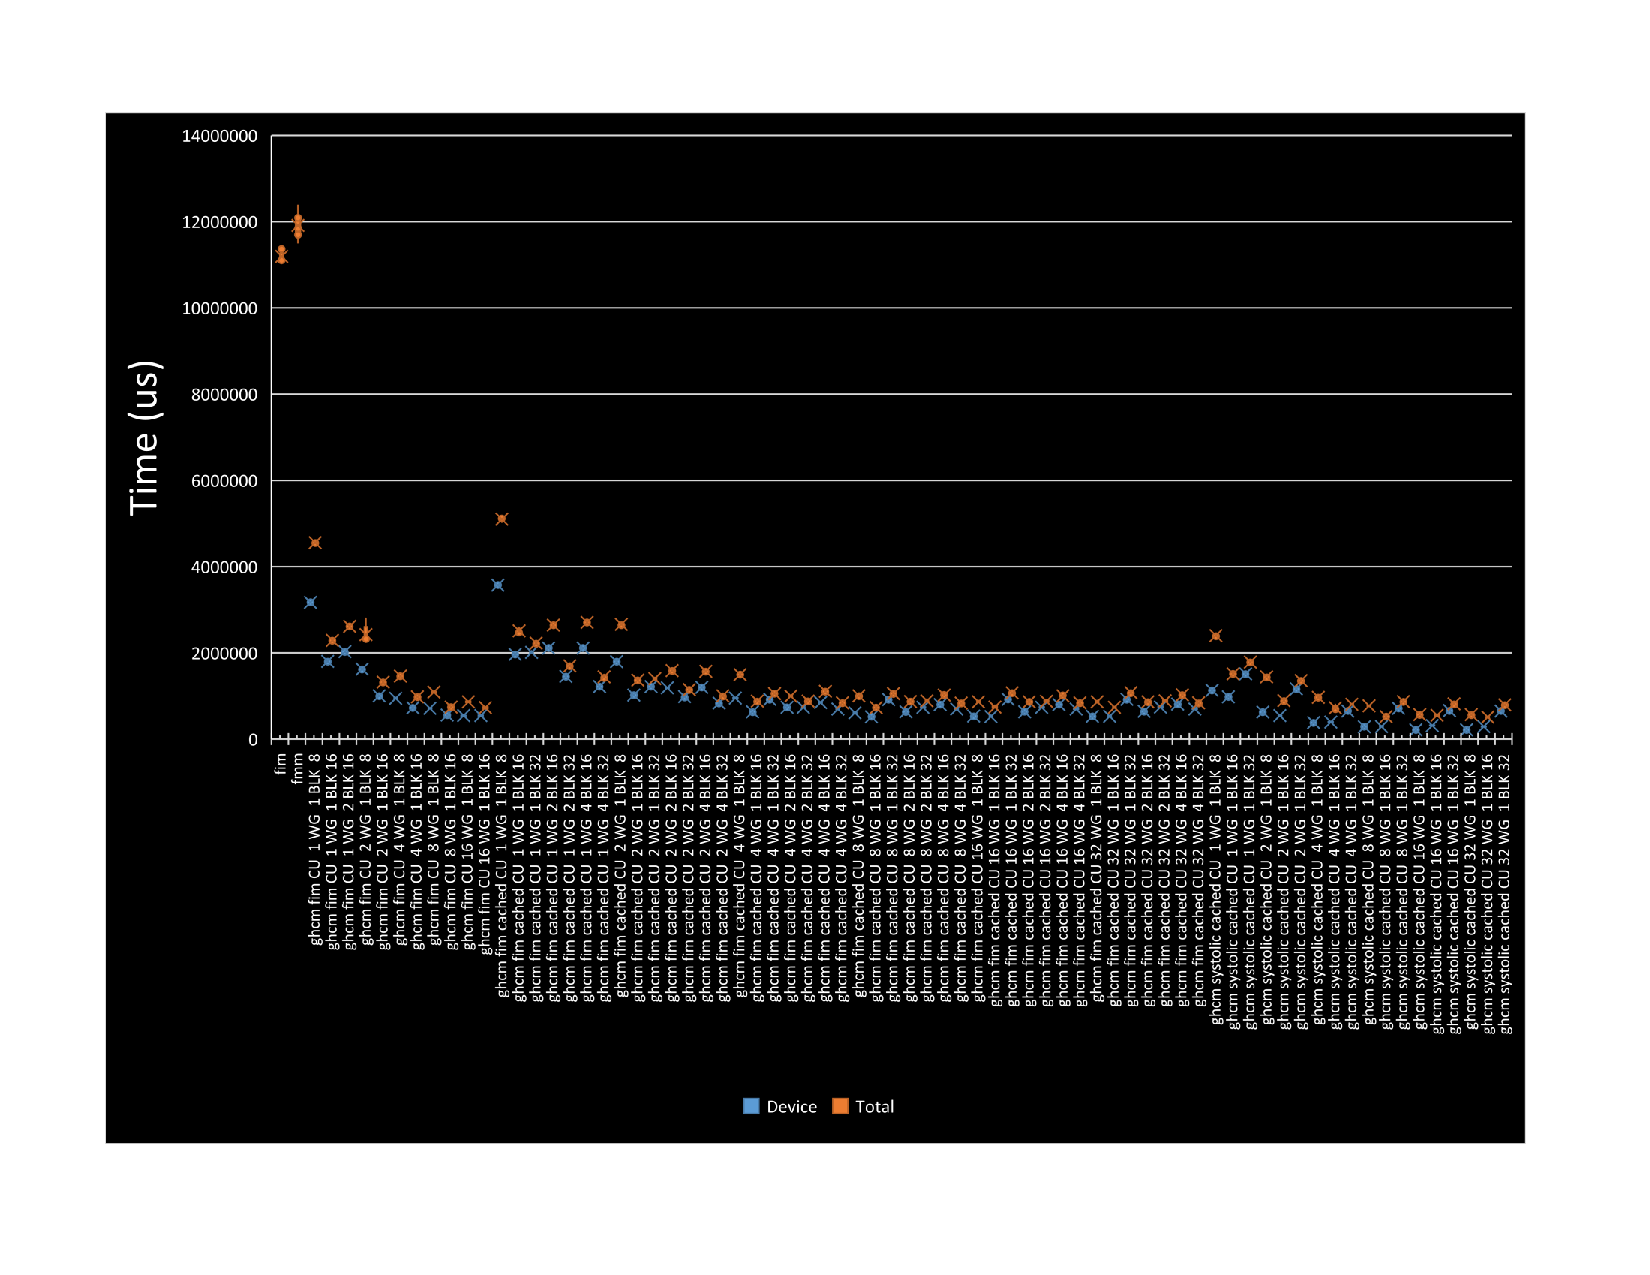
\includegraphics[width=\textwidth]{Figures/time-constant}
		\caption{Constant (Time)}
	\end{subfigure}
	\begin{subfigure}[b]{.4\columnwidth}
		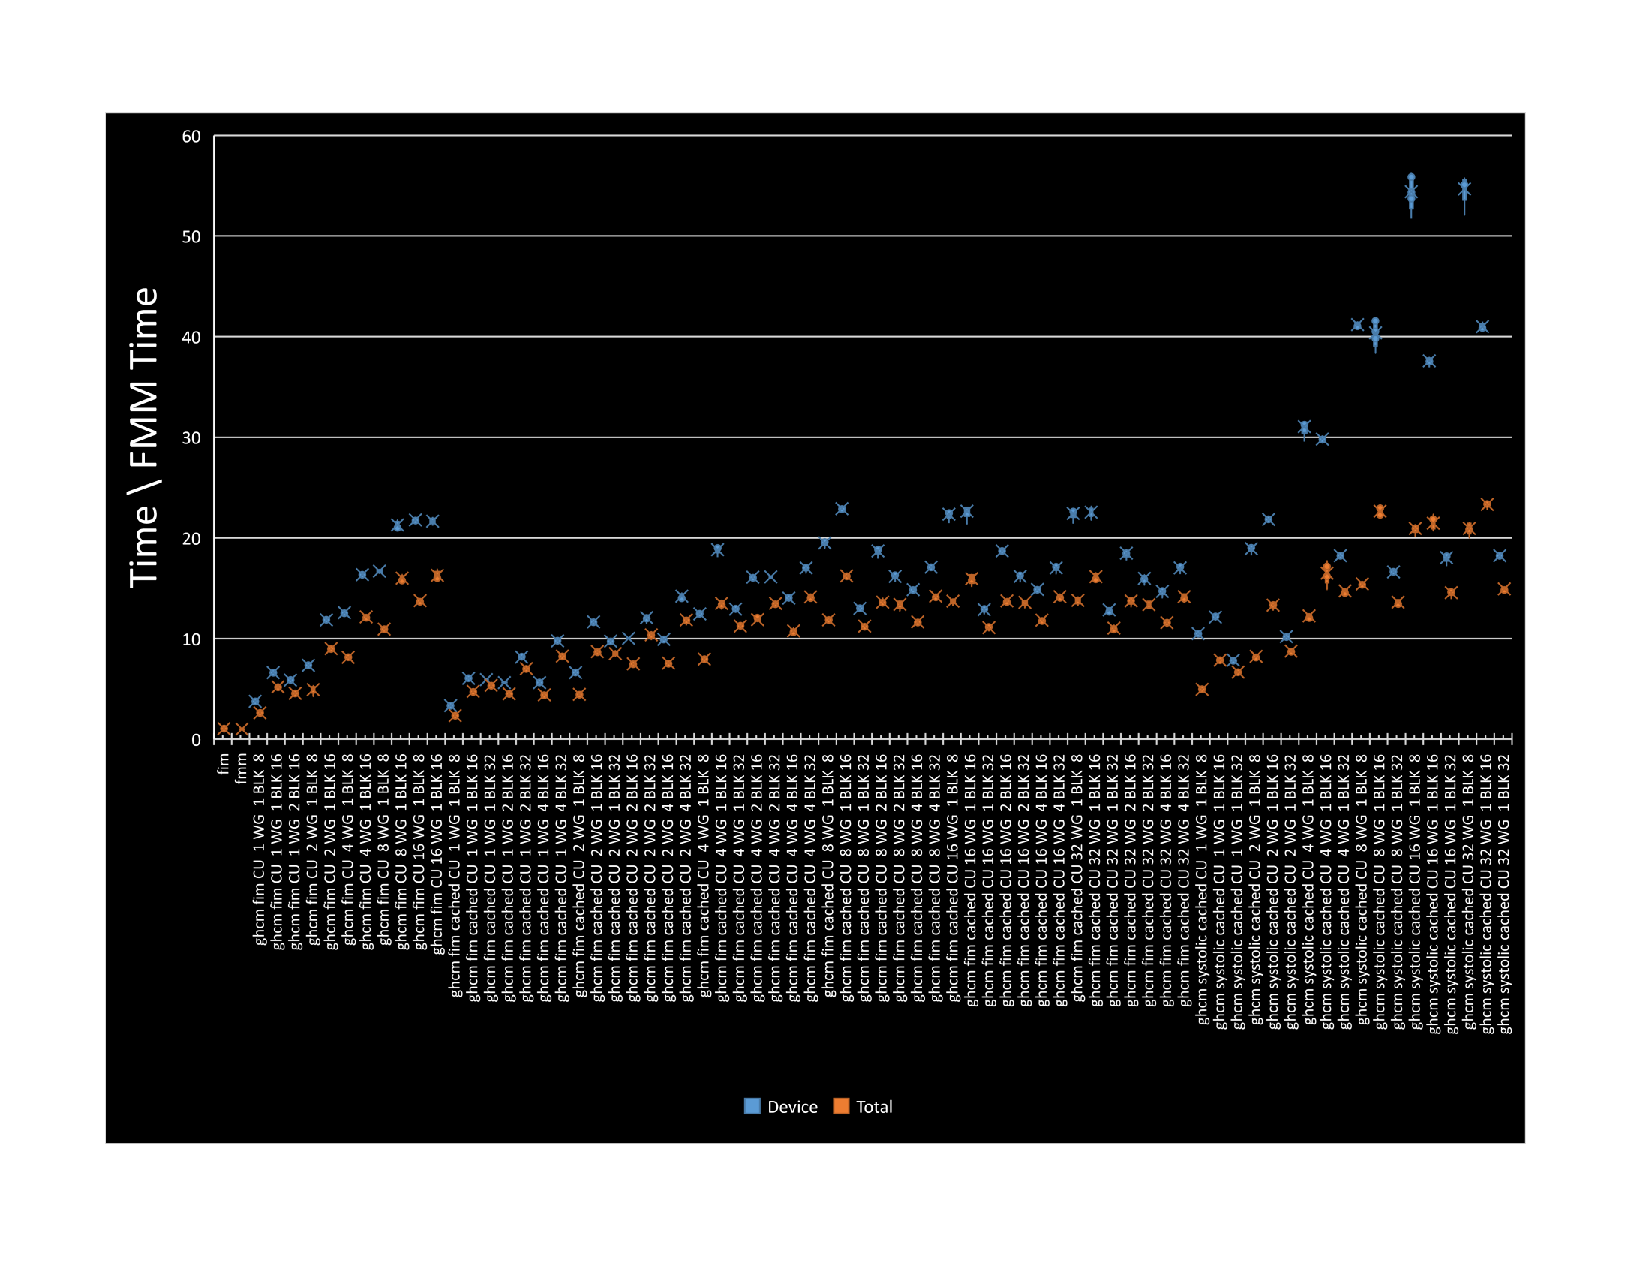
\includegraphics[width=\textwidth]{Figures/ratio-time-constant}
		\caption{Constant (Ratio)}
	\end{subfigure}

	\begin{subfigure}[b]{.4\columnwidth}
		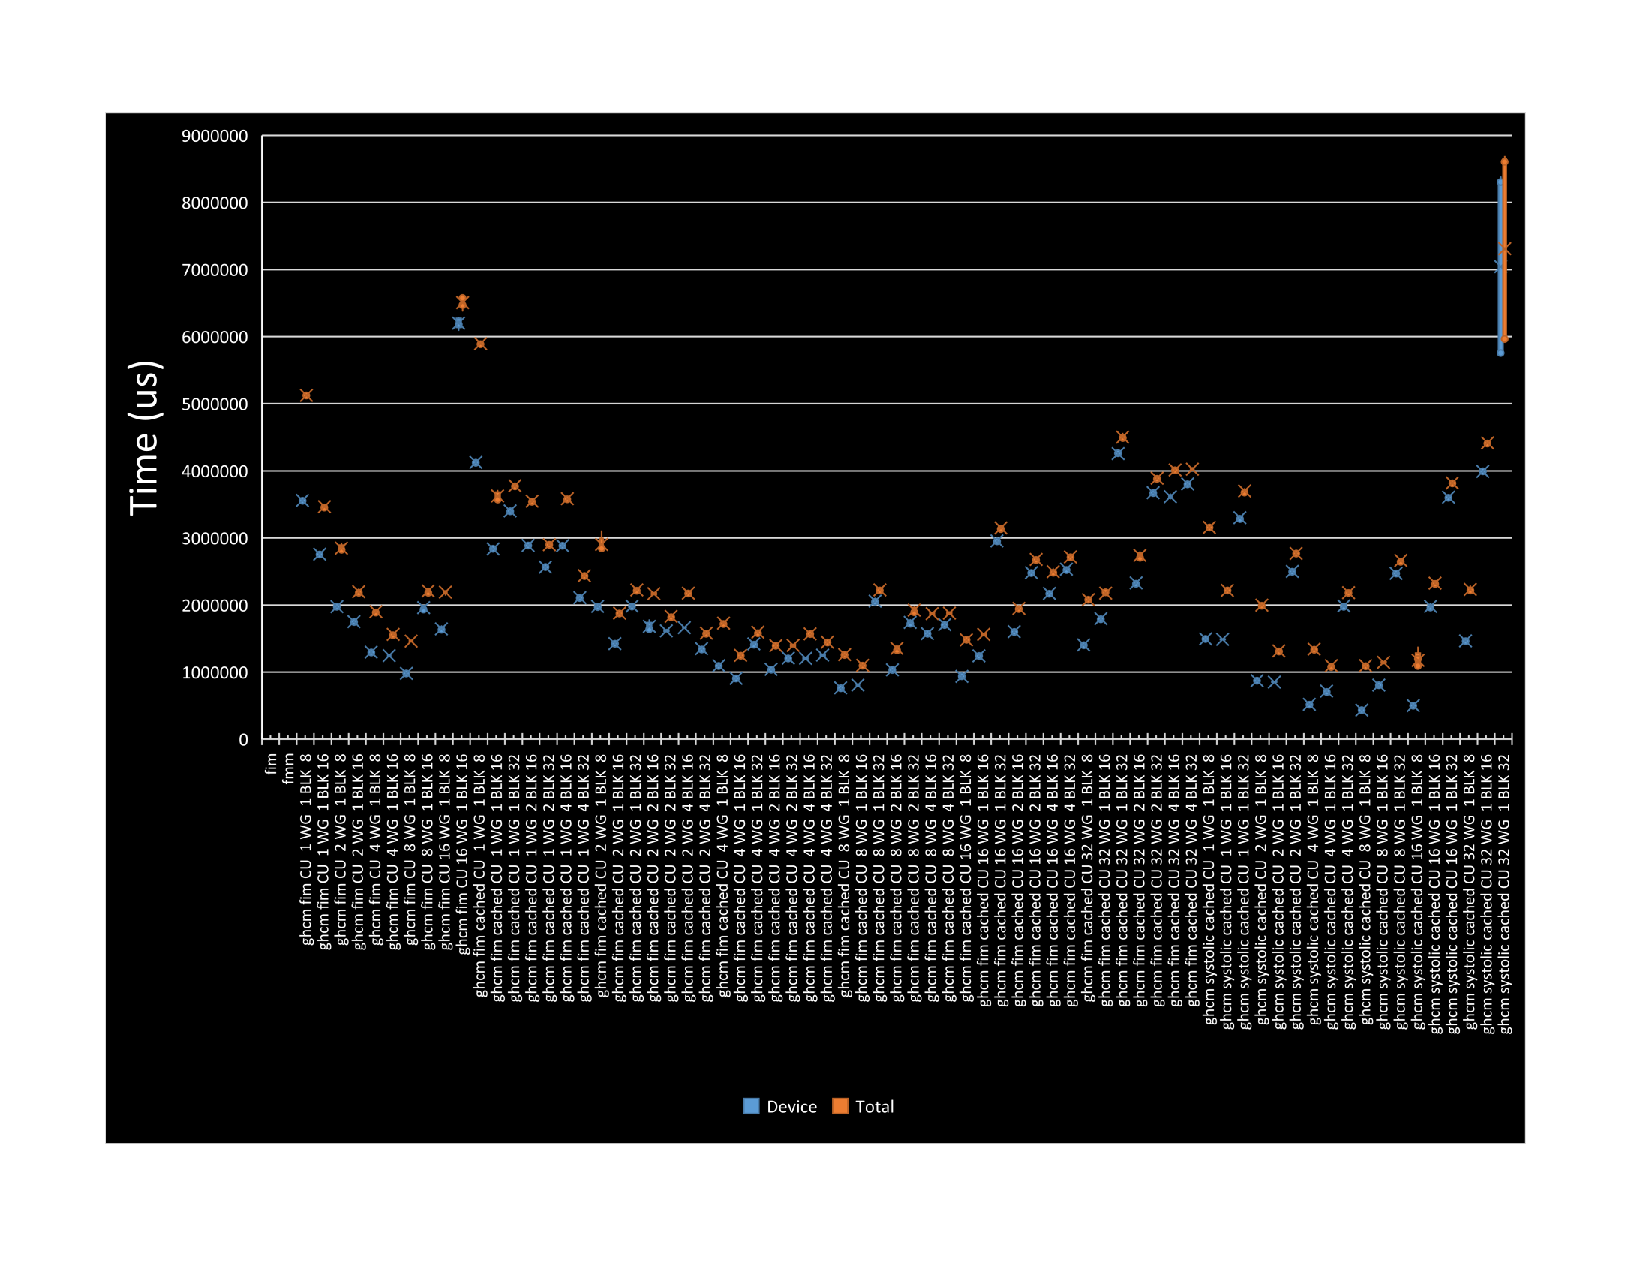
\includegraphics[width=\textwidth]{Figures/time-sin-checkerboard}
		\caption{Sin Checkerboard (Time)}
	\end{subfigure}
	\begin{subfigure}[b]{.4\columnwidth}
		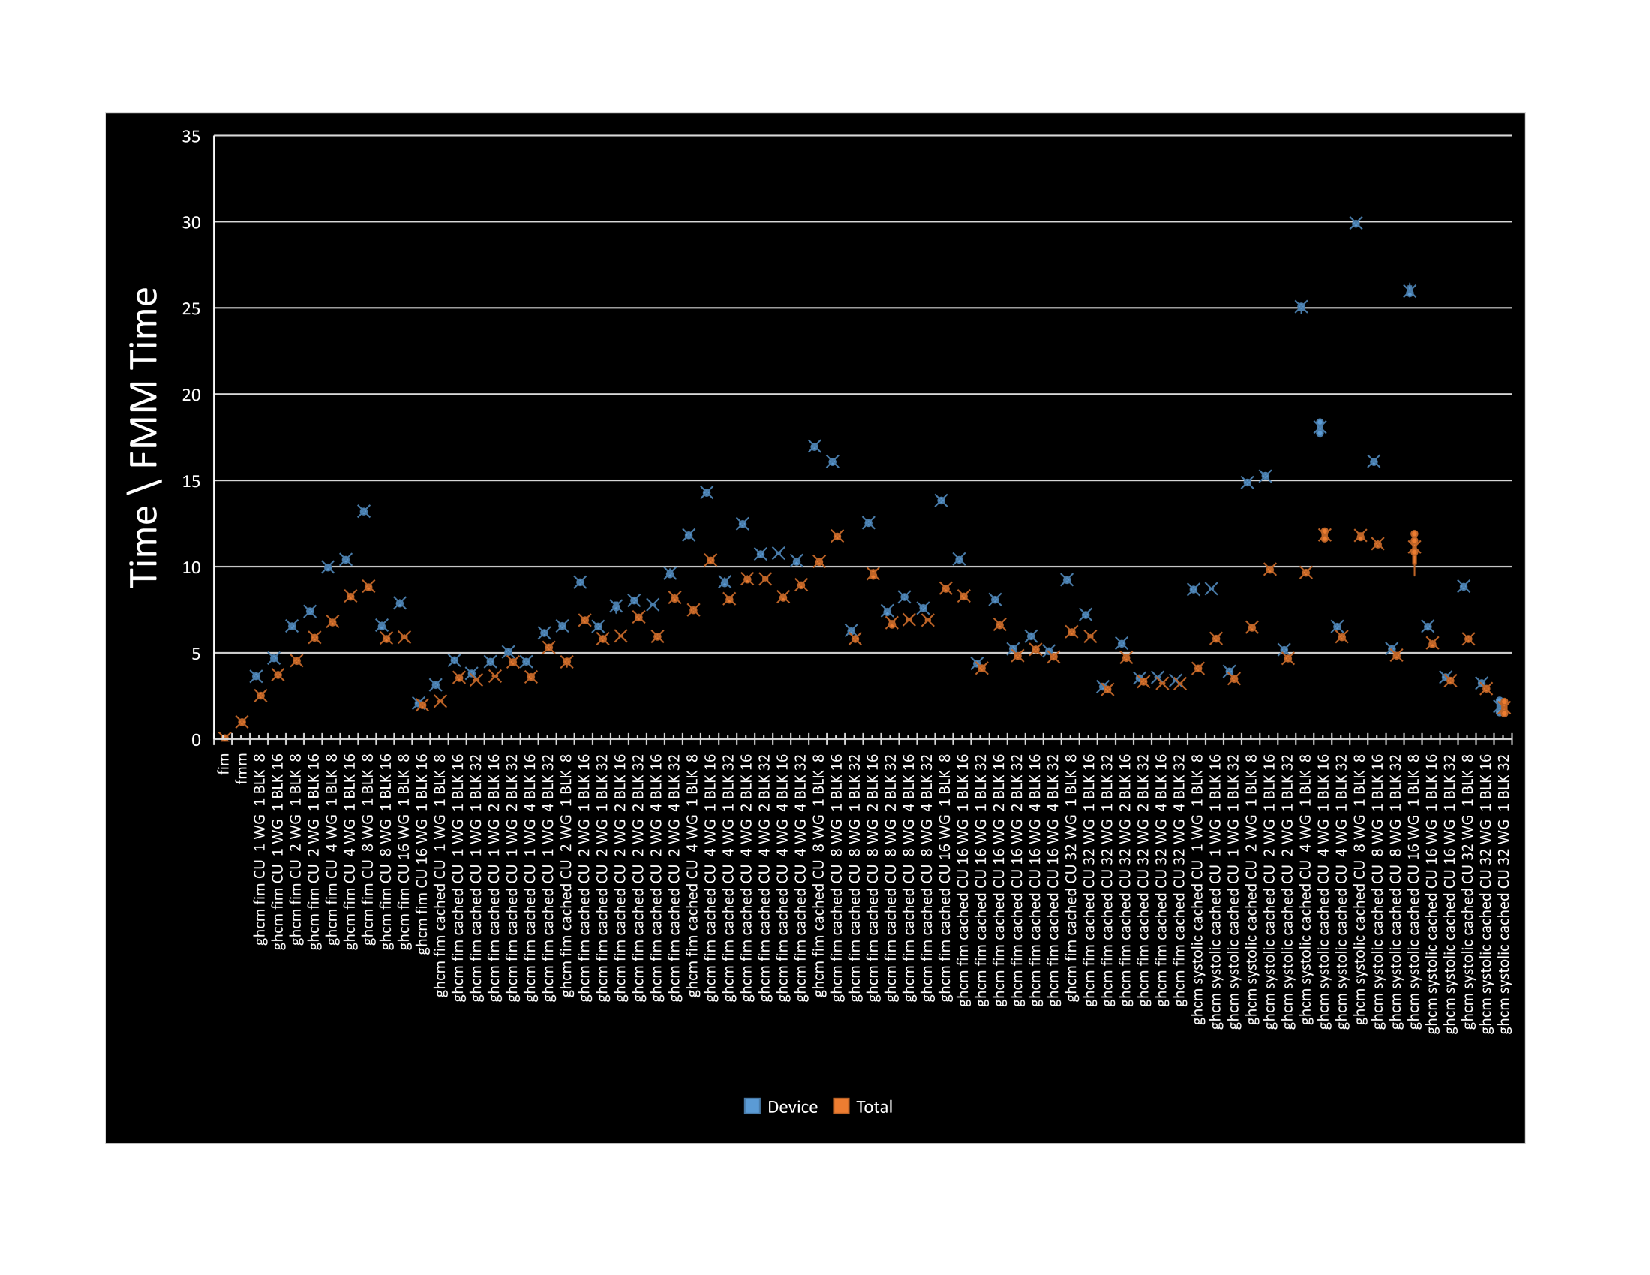
\includegraphics[width=\textwidth]{Figures/ratio-time-sin-checkerboard}
		\caption{Sin Checkerboard (Ratio)}
	\end{subfigure}

	\begin{subfigure}[b]{.4\columnwidth}
		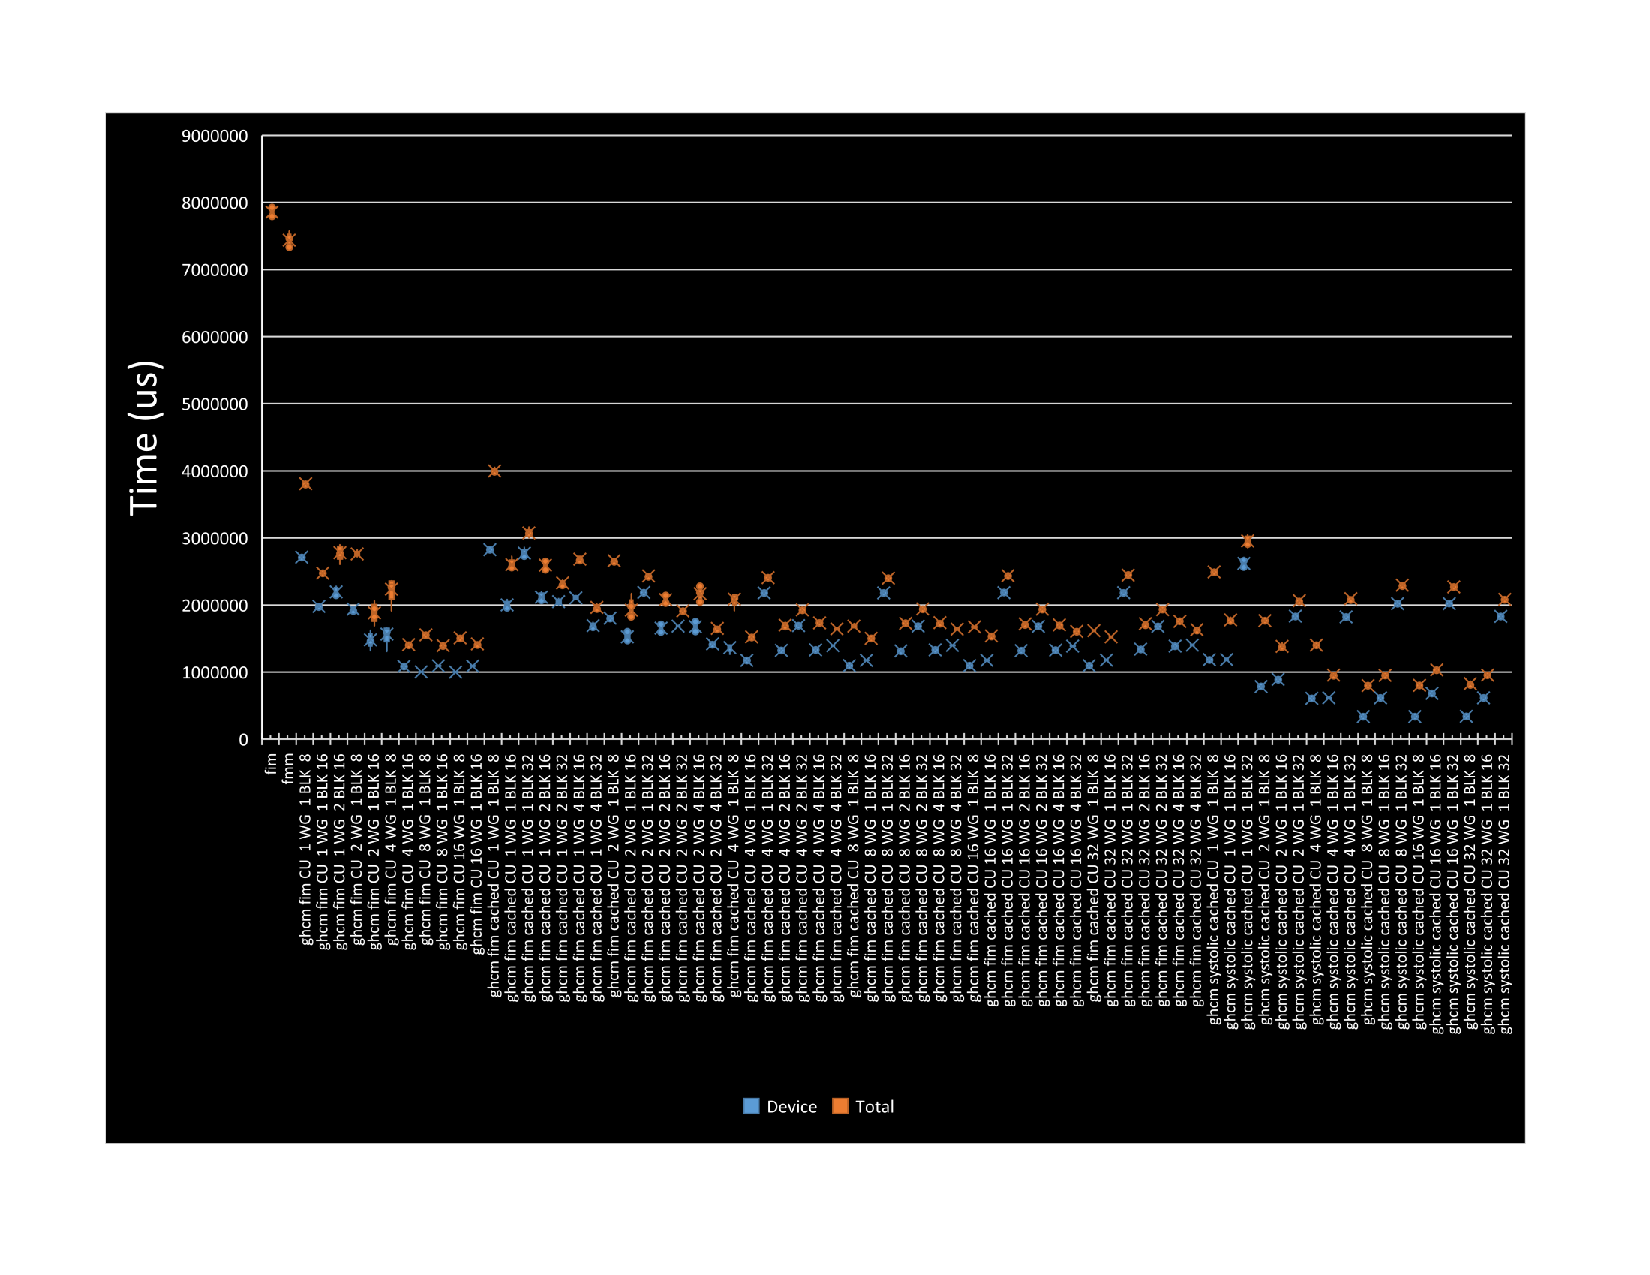
\includegraphics[width=\textwidth]{Figures/time-7-ring}
		\caption{7-Ring (Time)}
	\end{subfigure}
	\begin{subfigure}[b]{.4\columnwidth}
		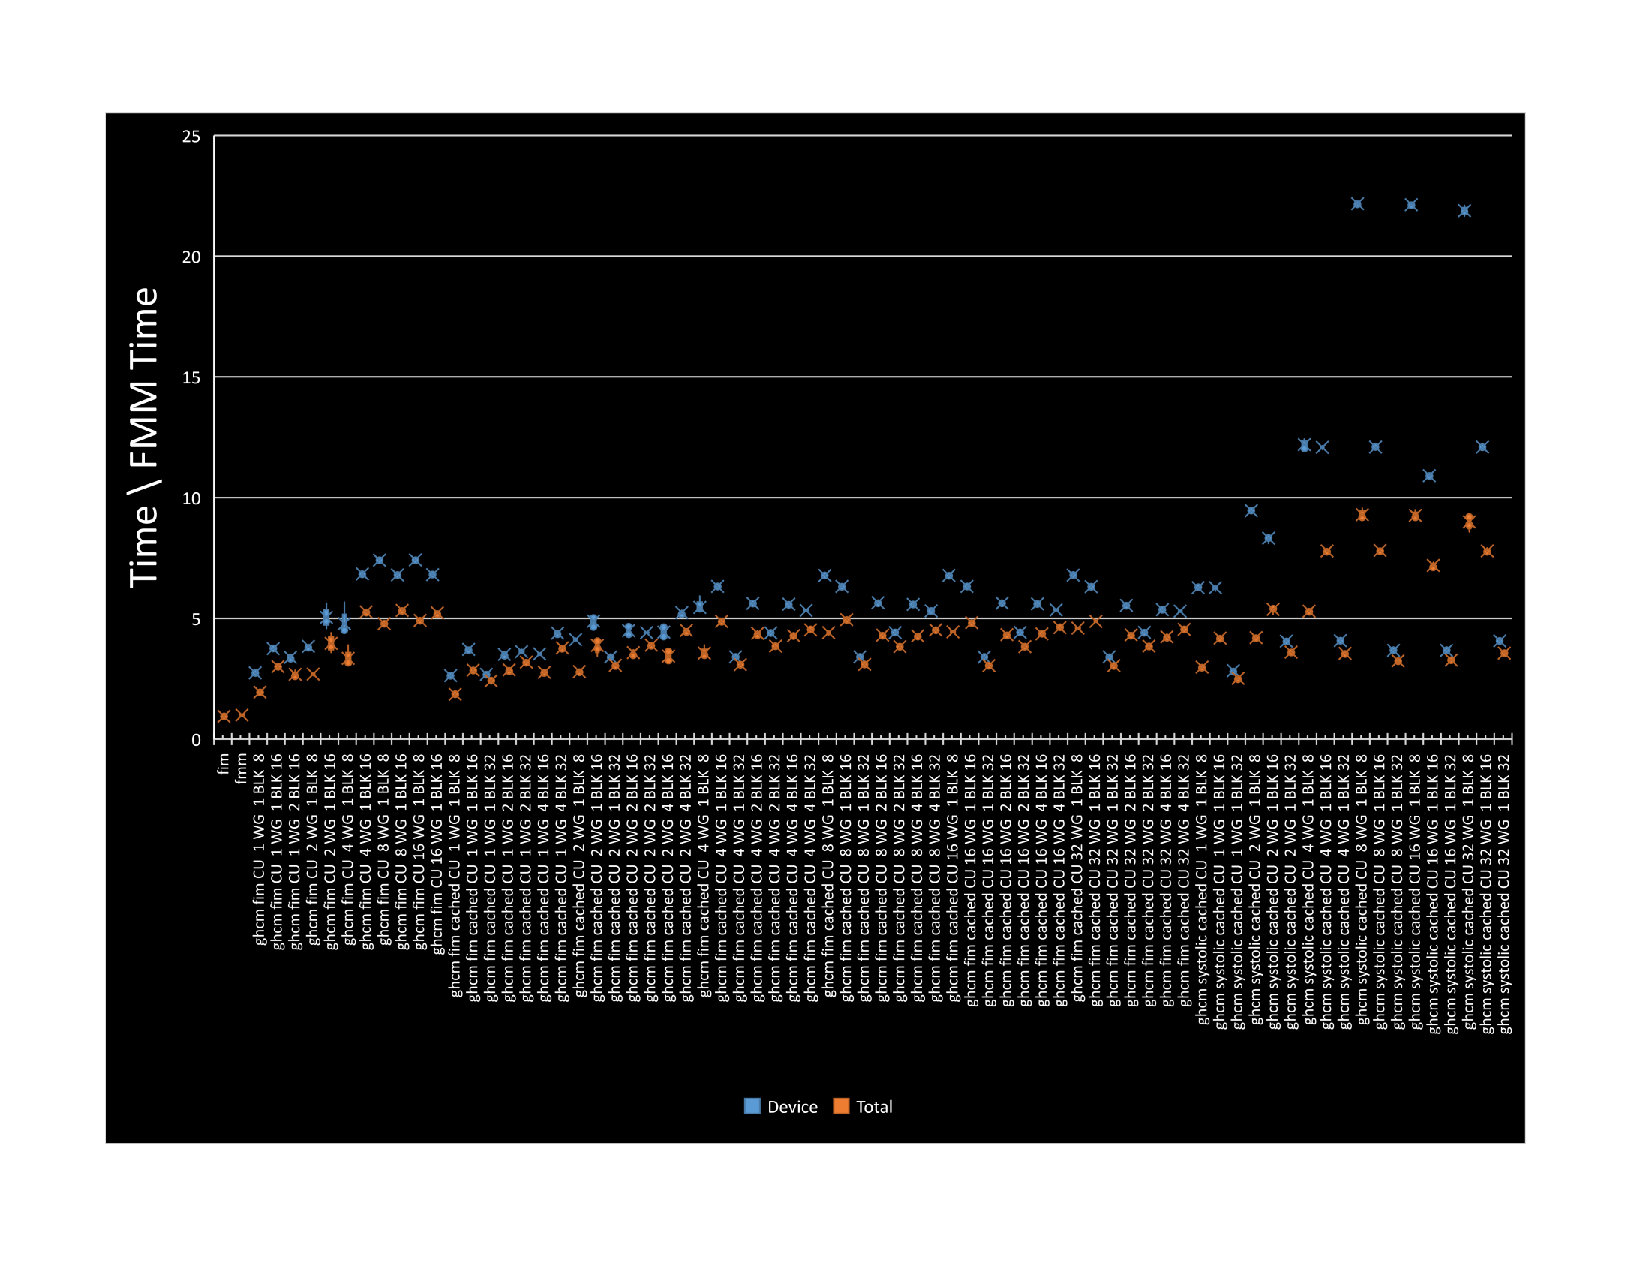
\includegraphics[width=\textwidth]{Figures/ratio-time-7-ring}
		\caption{7-Ring (Ratio)}
	\end{subfigure}

	\caption{Computation Time (in us) for Constant, Sin Checkerboard, and 7-Ring. Device time included for gHCM. If FIM time is missing from the absolute time plot, assume its three to four orders of magnitude worse than FMM. (1 of 2)}
	\label{fig:perf_results_main_1}
\end{figure}

\begin{figure}%[!b]
	\centering
	\begin{subfigure}[b]{.4\columnwidth}
		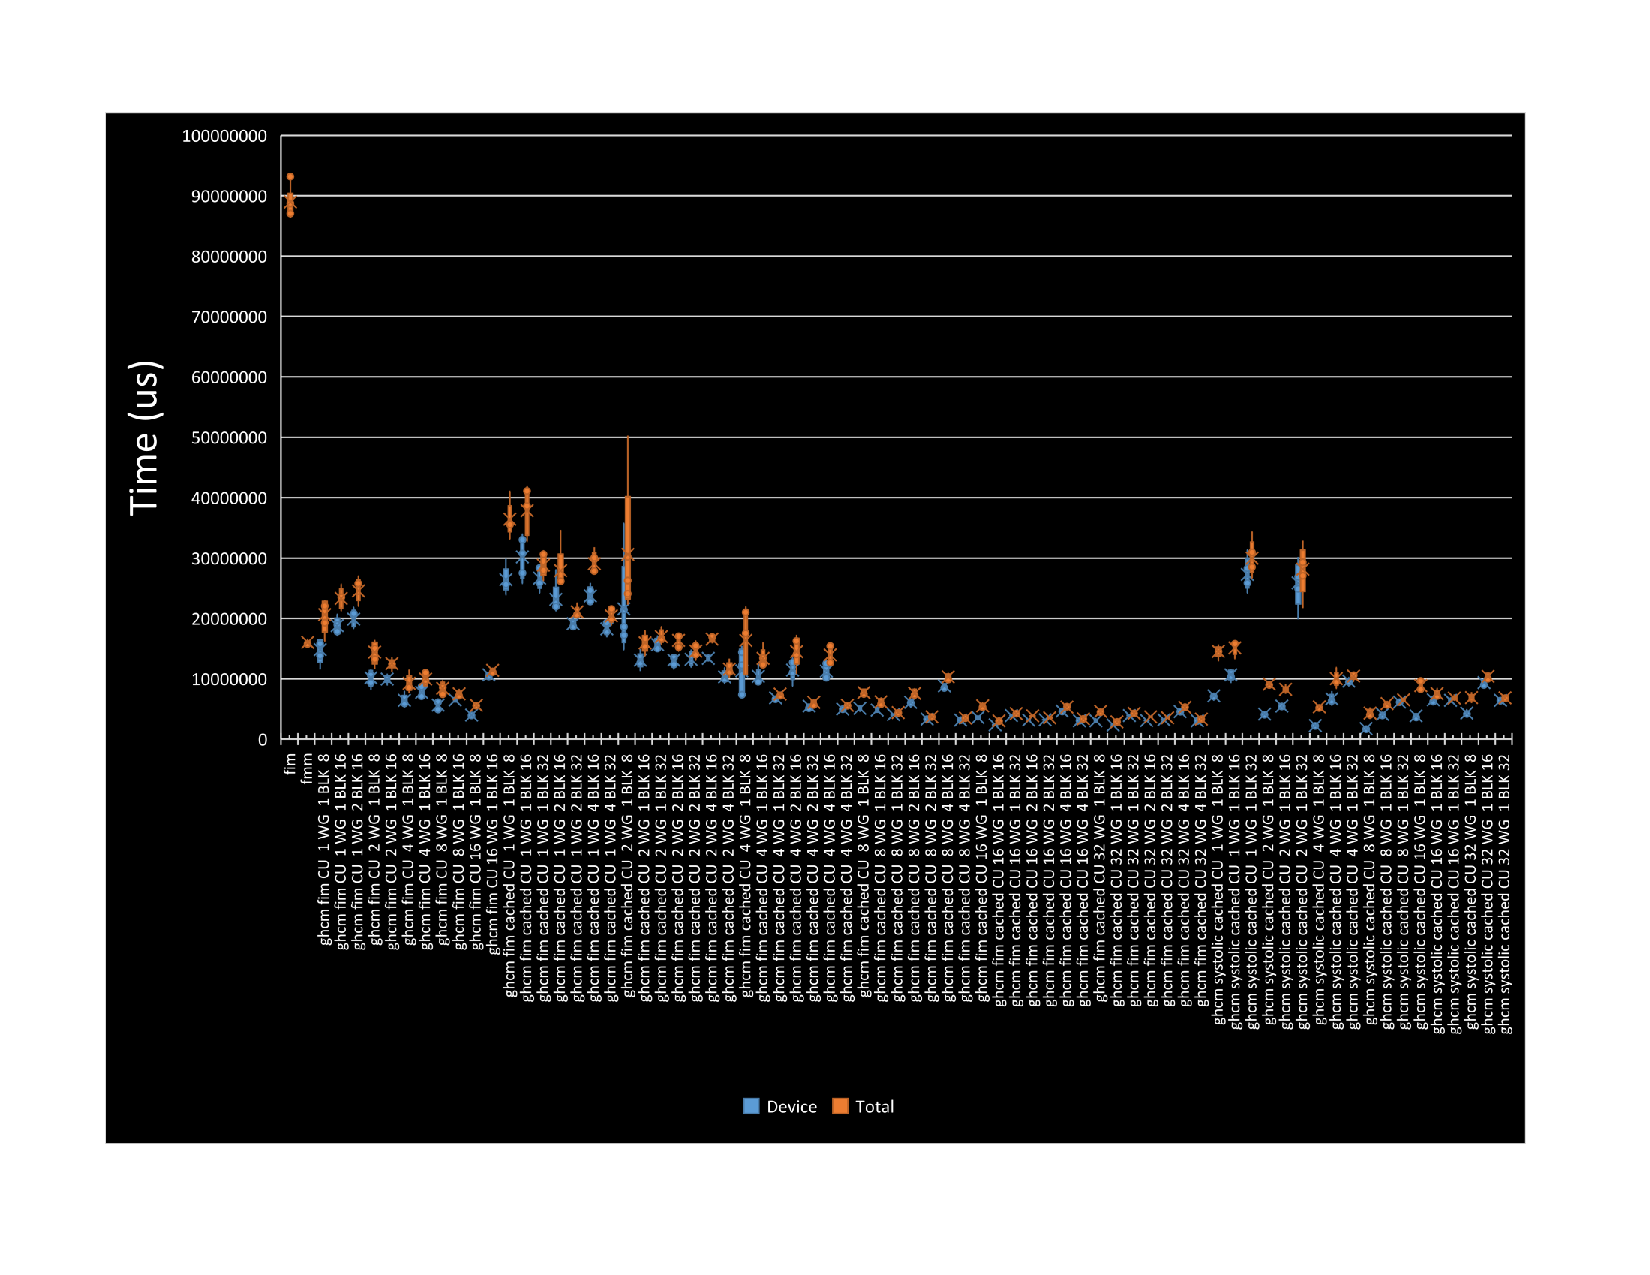
\includegraphics[width=\textwidth]{Figures/time-7-ring-permeable}
		\caption{7-Ring Permeable (Time)}
	\end{subfigure}
	\begin{subfigure}[b]{.4\columnwidth}
		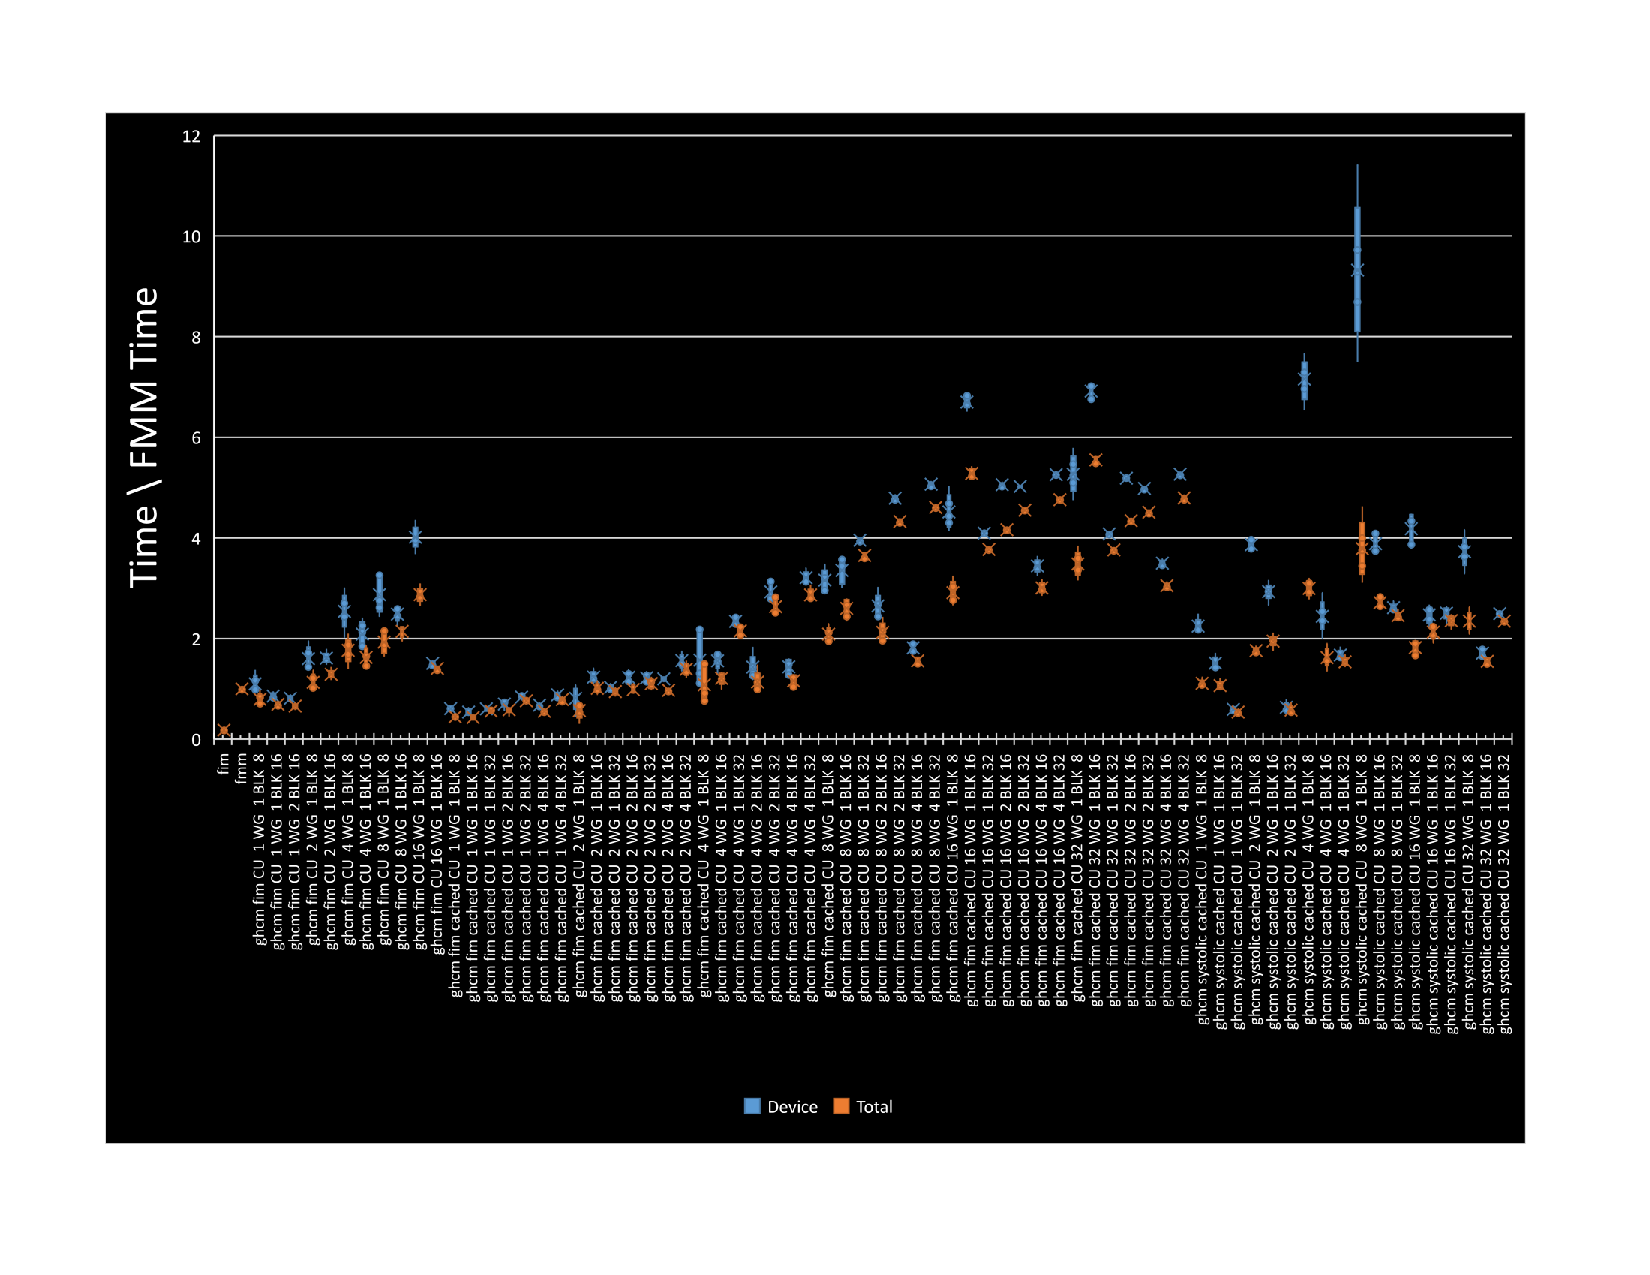
\includegraphics[width=\textwidth]{Figures/ratio-time-7-ring-permeable}
		\caption{7-Ring Permeable (Ratio)}
	\end{subfigure}
	
	\begin{subfigure}[b]{.4\columnwidth}
		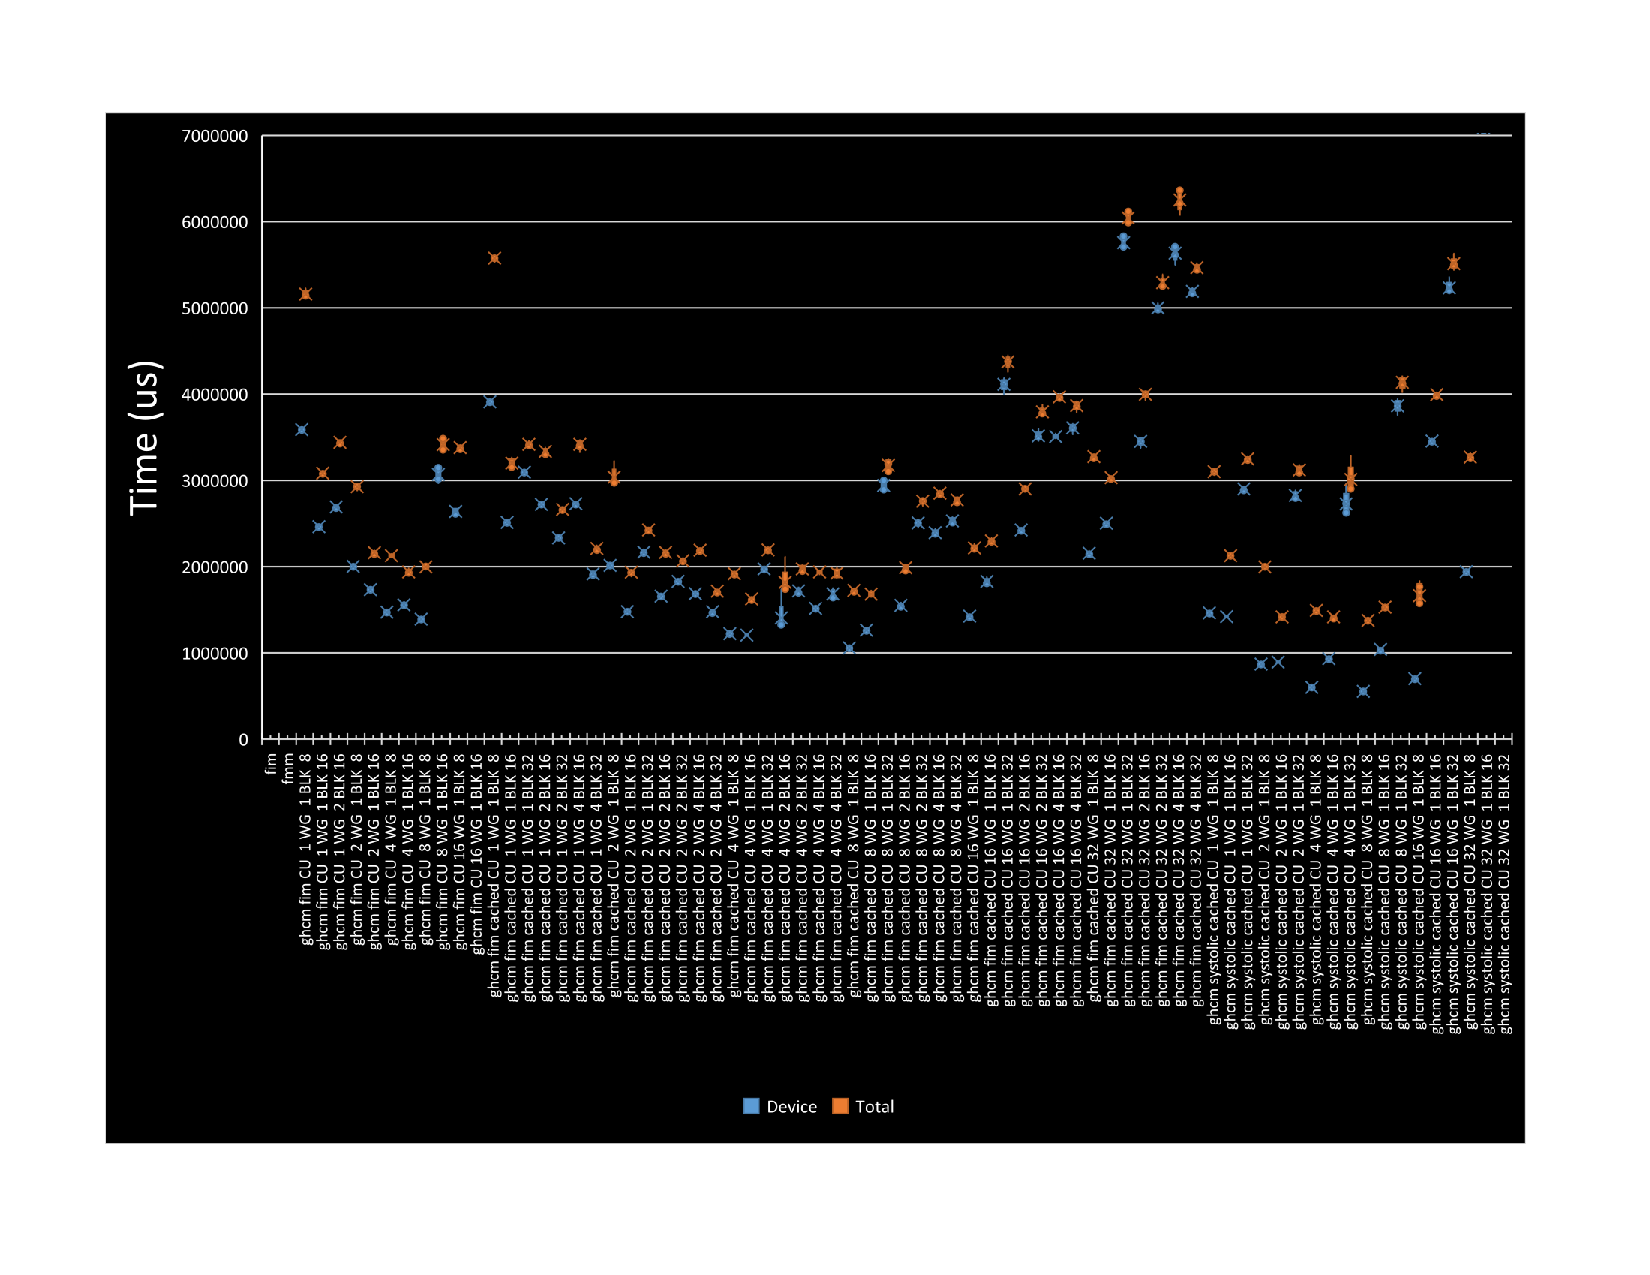
\includegraphics[width=\textwidth]{Figures/time-cloudy}
		\caption{Cloudy (Time)}
	\end{subfigure}
	\begin{subfigure}[b]{.4\columnwidth}
		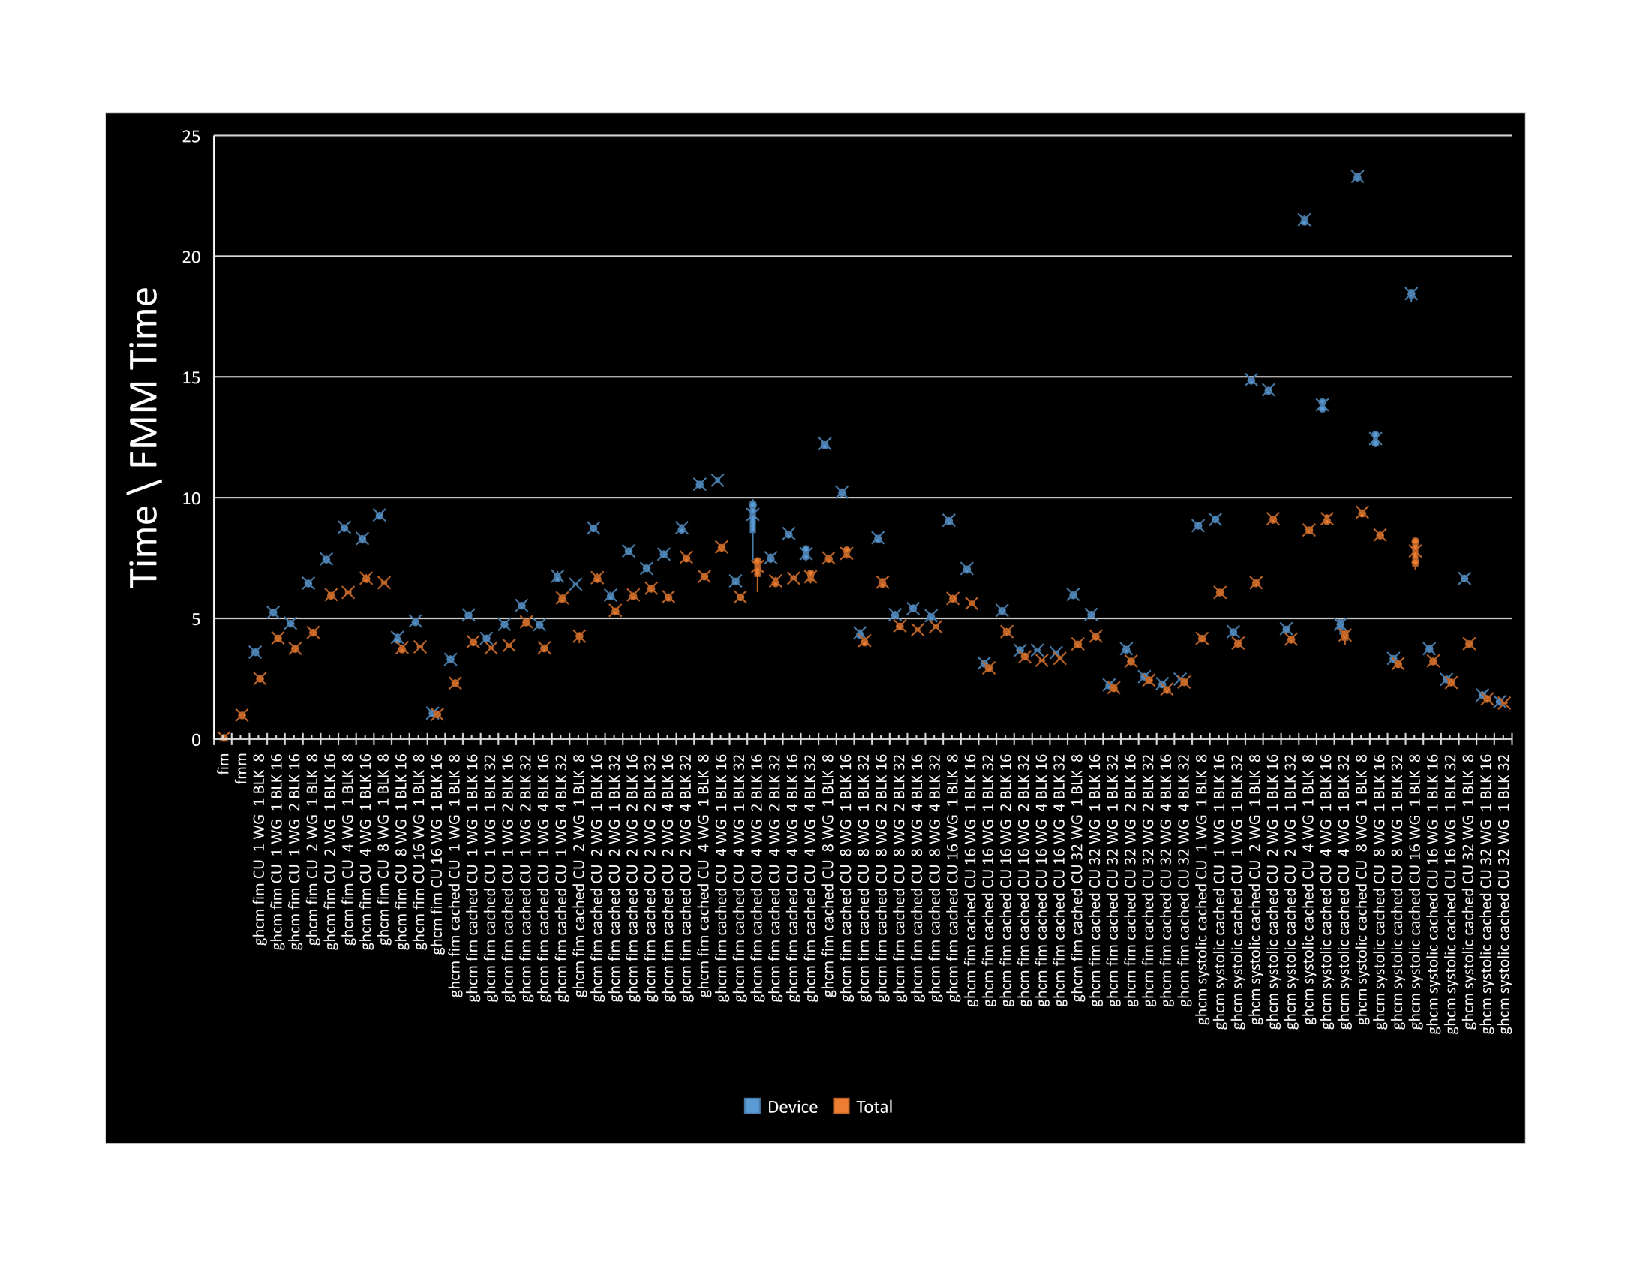
\includegraphics[width=\textwidth]{Figures/ratio-time-cloudy}
		\caption{Cloudy (Ratio)}
	\end{subfigure}
	
	\begin{subfigure}[b]{.4\columnwidth}
		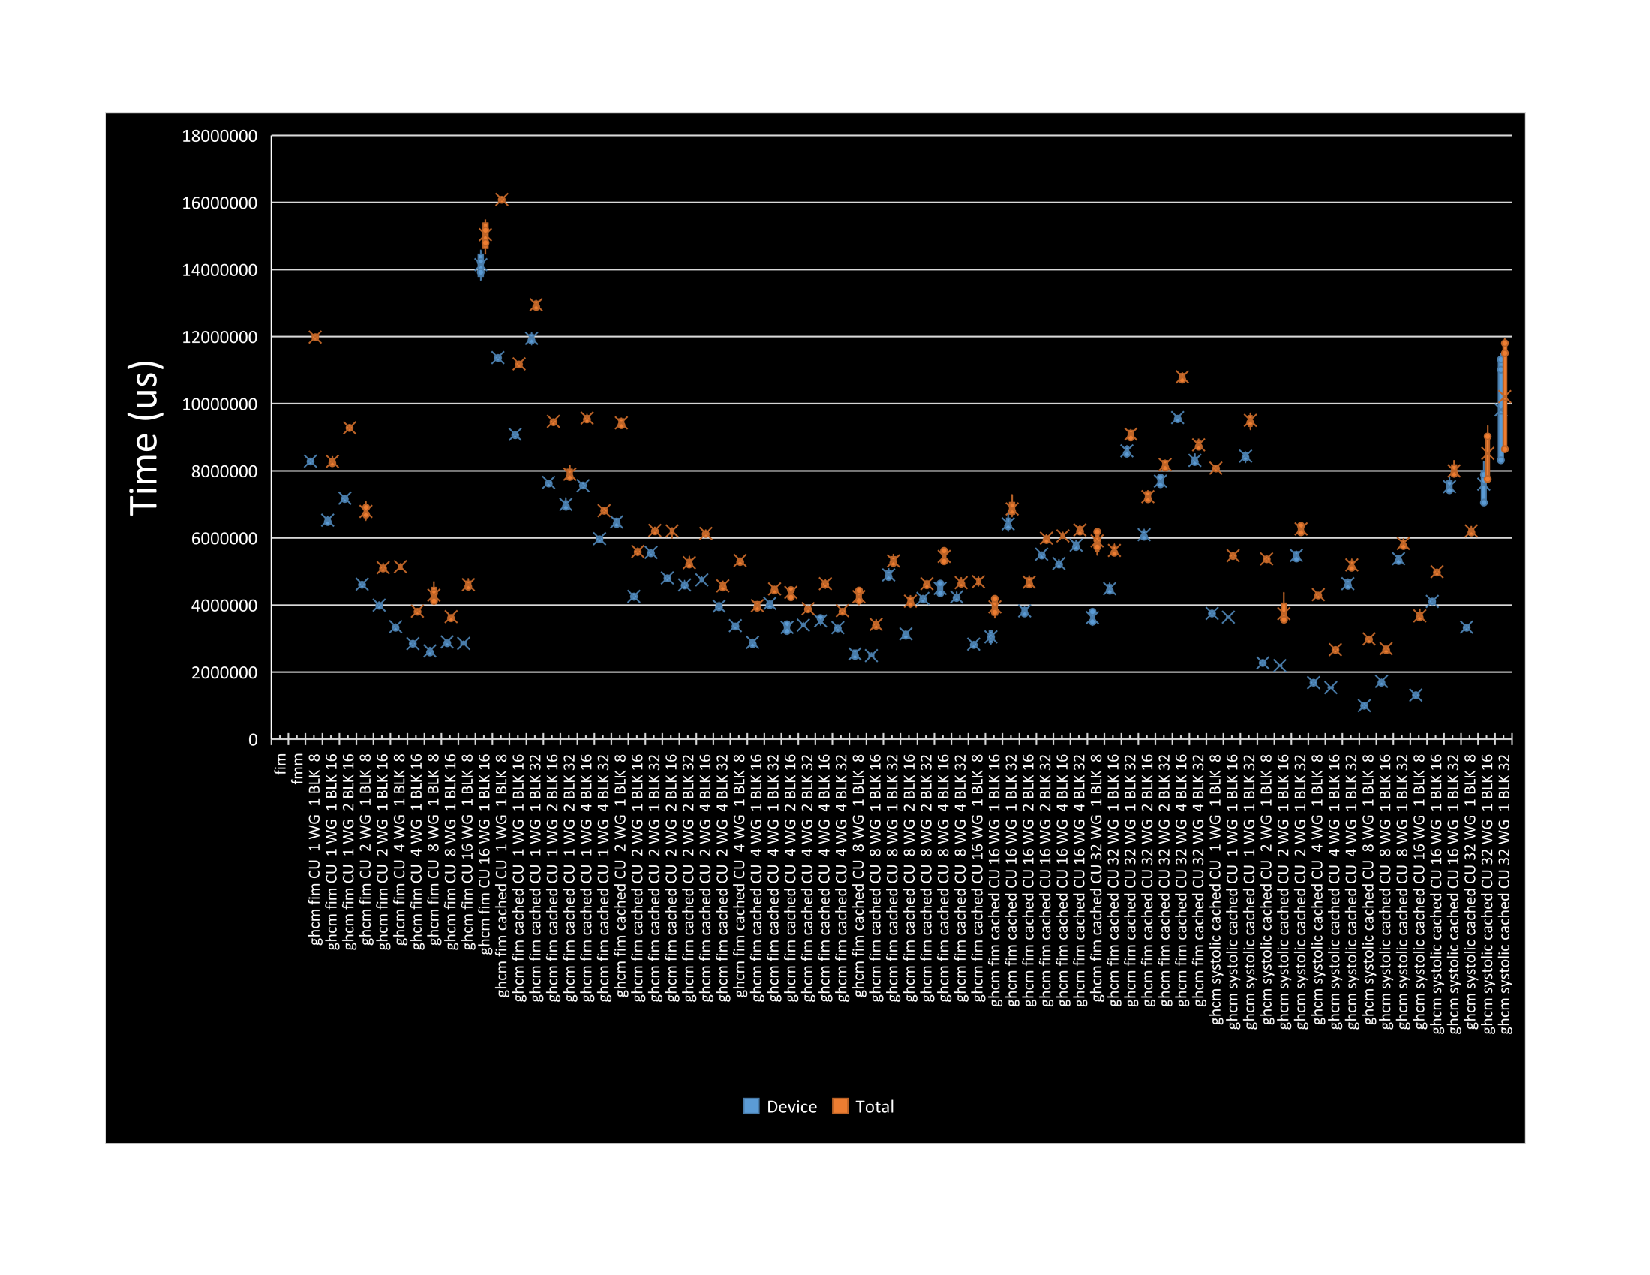
\includegraphics[width=\textwidth]{Figures/time-photo}
		\caption{Photograph (Time)}
	\end{subfigure}
	\begin{subfigure}[b]{.4\columnwidth}
		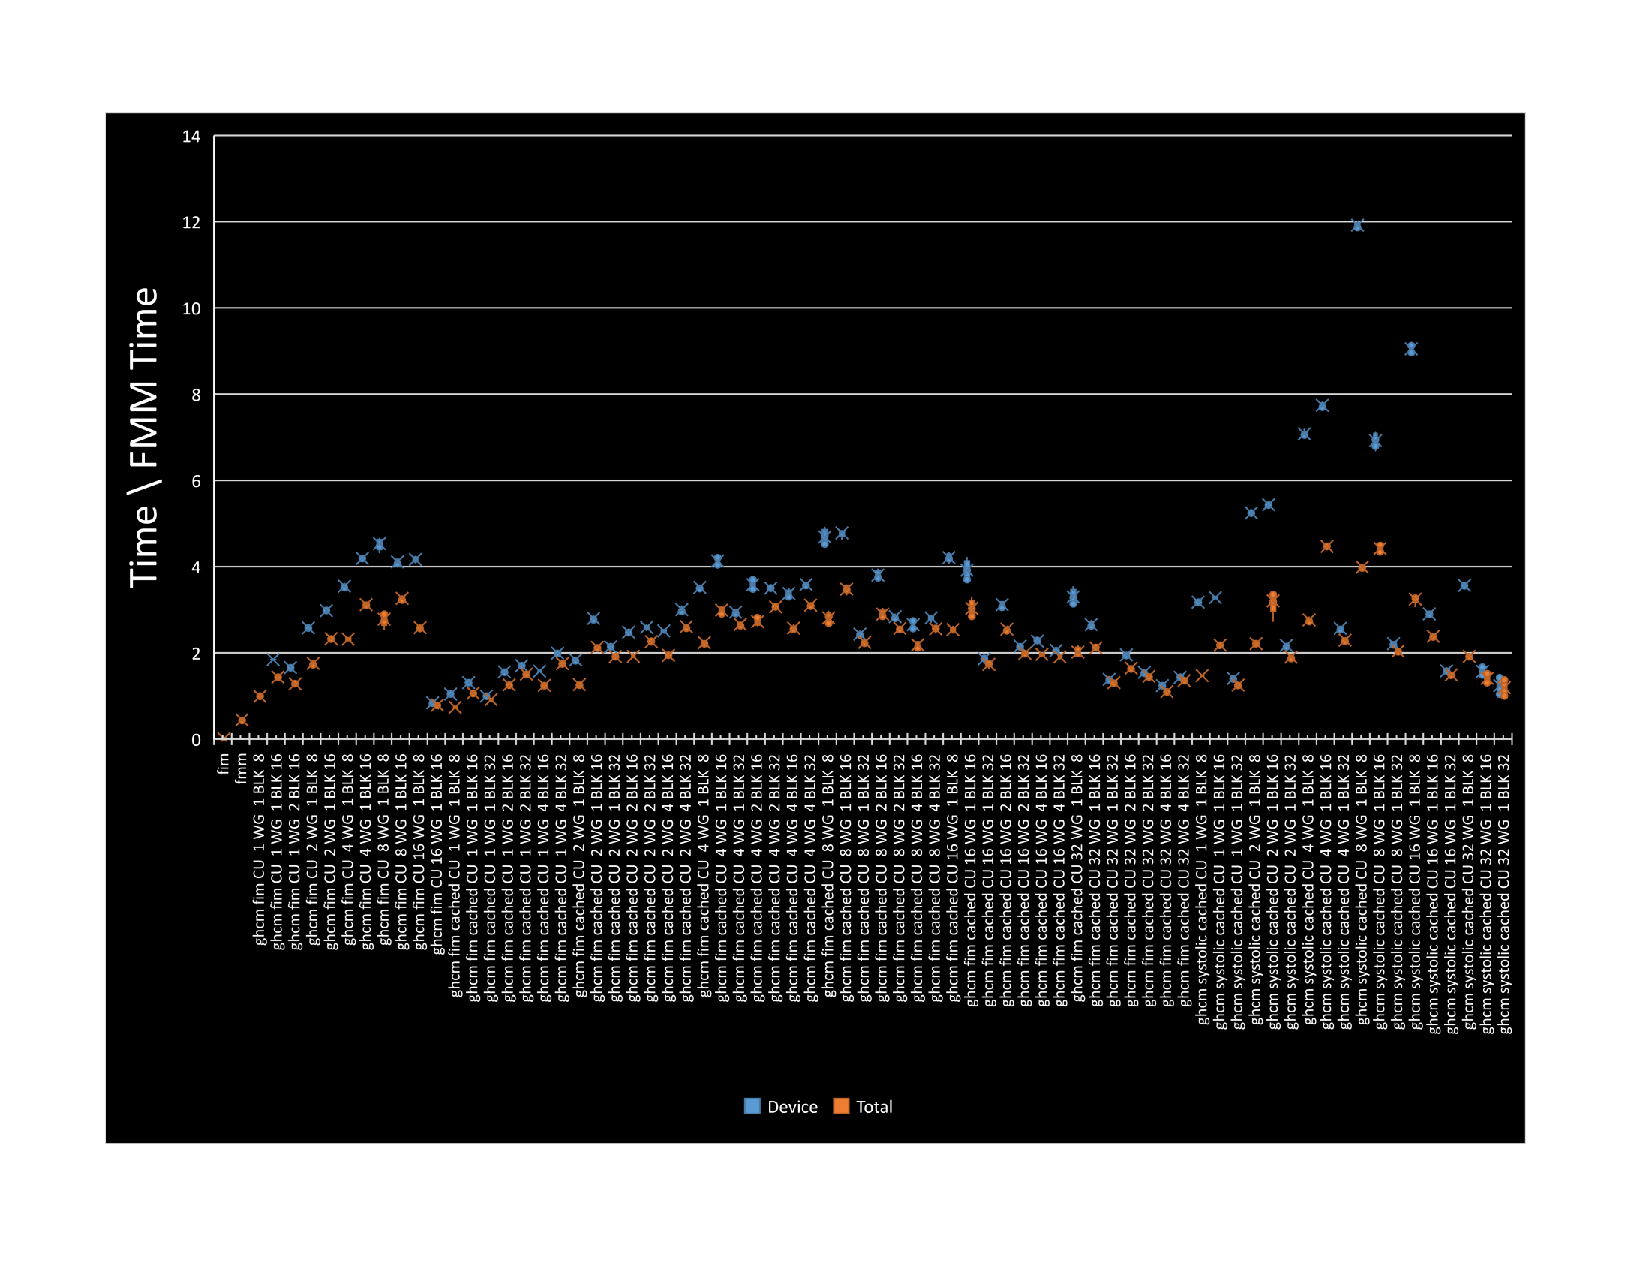
\includegraphics[width=\textwidth]{Figures/ratio-time-photo}
		\caption{Photograph (Ratio)}
	\end{subfigure}
	\caption{Computation Time (in us) for 7-Ring Permeable, Cloudy, and Photograph. Device time included for gHCM. If FIM time is missing from the absolute time plot, assume its three to four orders of magnitude worse than FMM. (2 of 2)}
	\label{fig:perf_results_main_2}
\end{figure}

\begin{comment}
\subsection{Kernel Configurations}
\begin{table}
	\centering
	\begin{tabular}{l r}
		
	\end{tabular}
	\begin{tabular}{|r|c|c|}
		\multicolumn{1}{c}{} & \multicolumn{1}{c}{Systolic-like} & \multicolumn{1}{c}{FIM}\\
		\cline{1-3} $\frac{\text{Work Items}}{\text{Workgroup Size}}$ 	& 1	& 4 \\

		\cline{1-3}
	\end{tabular}
	\caption{AMD Radeon R9 280x characteristics.}
	\label{tab:kernel_stats}
\end{table}
\end{comment}


% ############################################################################
\section{Conclusion} \label{sec:conclusion}
% ############################################################################

We implemented a modified version of FIM similar to HCM. This new scheme improves performance in a number of scenarios, but requires tuning to the hosting hardware and to a lesser degree the general nature of the problems being solved. We also tested two block-solving kernels: one systolic-styled, and the other an implementation of FIM. We expected the simplicity of the systolic kernel to be more effective, but the FIM kernel proved competitive than we had anticipated. Our implementation has not had much work given to optimisation. (See \autoref{fig:perf_results_main_2}, 7-Ring Permeable.) We only had time to do some simple OpenCL API tweaks, and we believe some notable gains could be had with a bit of polish on both CPU and GPU ends.

During testing, we encountered a few instances where gHCM failed to converge as well deadlocks in the OpenCL runtime. Some of these were found to be bugs in our code, but the rest remain a mystery. Given the difficultly of reproducing these issues with a debug kernel, and the fact that our hosting system seems prone occasional HW failure\footnote{The bloody thing occasionally panics with HW faults reported by the kernel. Honestly I don't know if this is due to slightly flaky hardware (quite possible, my RAM doesn't perform at its full rated speed, and the GPU occasionally manifests texture corruption), magic gamma rays, or terrible drivers.}, we've not manage to investigate this to our satisfaction.

Possible future work includes: deriving a more precise model for balancing compute-unit overload, investigating if GMM could be a good replacement for the priority heap in gHCM, investigating if and how device-side kernel en-queuing might be exploited (might it possible to effectively drive gHCM on-device?), and testing to see if the texture systems on the GPU can be exploited to obtain better memory locality without resorting to manual z-ordering.

\begin{comment}
priority scheduling of blocks is indeed worthwhile on larger problems
	particularly on pathological problems
		-> FIM just dies in the open list mire
		-> hybrid powers through

debugging GPU kernels is a bitch
	emitted assembly is available (unlike NV)
		but utterly indecipherable without manual open at all times
	kernel profiling is limited

possible bugs in FIM impl (or faulty hardware? unsure.)

explicit caches turned out to be pointless, HW/autocaching is clever enough to do it for us

future work:
	current scheduler is dumb as nails
		-> augment w/ 



The ``moral of the story'': What have we learned? What did we achieve?
What did we not achieve? What would we do better next time? Possibilities
for future research...
\end{comment}
% ############################################################################
% Bibliography
% ############################################################################

\nocite{rouy1992viscosity}
\nocite{kim2001levelset}
\nocite{bak2010some} % Locked Sweeping Method
\nocite{blelloch90prefixsums}

\bibliographystyle{plain}
\bibliography{my-bibliography}     %loads my-bibliography.bib

% ============================================================================
\end{document}
% ============================================================================
